




\documentclass[spanish,openright]{book}







\synctex=1

\usepackage{ifthen}

\newcommand{\colorspaceused}{rgb}

\ifthenelse{\equal{\colorspaceused}{rgb}}
{
  \PassOptionsToPackage{rgb}{xcolor}}
{
  \PassOptionsToPackage{cmyk}{xcolor}}

\usepackage[utf8]{inputenc} \usepackage[T1]{fontenc}      \usepackage{ae}               \usepackage{lmodern}          


\usepackage{wrapfig}
\usepackage{lipsum}

\usepackage[final]{pdfpages}

\usepackage{emptypage}

\usepackage{tocbibind}

\usepackage{listings}
\usepackage{longtable}
\usepackage{afterpage}

\usepackage{xspace}
\usepackage{verbatim}
\usepackage{moreverb}
\usepackage{multicol}
\usepackage{amsmath}
\usepackage{eurosym}
\usepackage{multirow}
\usepackage{fancyhdr}
\usepackage{makeidx}
\usepackage{rotating}
\usepackage{supertabular}
\usepackage{hhline}
\usepackage{array}
\usepackage[noadjust]{cite}      


\usepackage[center]{caption}
\usepackage{subcaption}

\usepackage{xcolor}




\definecolor{pantone293}{RGB}{35,91,168}

\definecolor{headingPortadaTFG}{RGB}{152,118,52}
\definecolor{headingPortadaTFM}{RGB}{0,90,170}
\definecolor{textoHeadingPortadaTFM}{RGB}{208,205,102}
\definecolor{textoHeadingPortadaTFG}{RGB}{208,205,102}

\definecolor{gray97}{gray}{.97}
\definecolor{gray75}{gray}{.75}
\definecolor{gray45}{gray}{.45}




\usepackage{tikz}




\usepackage{geometry}
\geometry{verbose,a4paper,tmargin=2.5cm,bmargin=2.5cm,lmargin=2.5cm,rmargin=2.5cm}




\usepackage[
bookmarks=true,bookmarksnumbered=true,            hypertexnames=false,               breaklinks=true,                   linktoc=all,
colorlinks=true,
linkcolor=blue,    
citecolor=green,
urlcolor=blue,                     pdfborder={0 0 112.0},              hyperfootnotes=false,
]{hyperref}                        

\setcounter{secnumdepth}{5}
\setcounter{tocdepth}{5}
\setcounter{table}{1}
\setcounter{figure}{1}
\setcounter{secnumdepth}{4}


\setlength{\parskip}{1ex plus 0.5ex minus 0.2ex}


\usepackage{multirow}

\usepackage{setspace}
\newcommand{\mycaptiontable}[1]{
  \begin{spacing}{0.6}
\begin{quote}
{{Table} \thechapter.\arabic{table}: #1}
\end{quote}
\end{spacing}
  \stepcounter{table}
}

\newcommand{\mycaptionfigure}[1]{
\begin{spacing}{0.6}
    \begin{quote}
{{Figure} \thechapter.\arabic{figure}: #1}
\end{quote}
\end{spacing}
  \stepcounter{figure}
}

\usepackage{amsmath}

\usepackage{courier}

\usepackage{multirow}
\usepackage{rotating}
\usepackage{setspace, amssymb, amsmath, epsfig, multirow, colortbl, tabularx}

\usepackage[acronym,shortcuts,nomain,hyperfirst=false]{glossaries}



\newcommand{\clearemptydoublepage}{\newpage{\pagestyle{empty}\cleardoublepage}}

\pagestyle{fancy}

\providecommand\phantomsection{}
\onehalfspacing
\sloppy  

\renewcommand{\chaptermark}[1]{\markboth{\chaptername\ \thechapter.\ #1}{}}
\renewcommand{\sectionmark}[1]{\markright{\thesection\ #1}{}}

\fancyhf{}

\fancyhead[LE,RO]{\bfseries\thepage}
\fancyhead[LO]{\bfseries\rightmark}
\fancyhead[RE]{\bfseries\leftmark}

\makeatletter
\renewcommand{\chaptermark}[1]{\markboth{\@chapapp \ \thechapter . \ #1}{}}
\renewcommand{\sectionmark}[1]{\markright{\thesection \ \ #1}}
\makeatother

\renewcommand{\headrulewidth}{0.5pt}
\renewcommand{\footrulewidth}{0pt}
\addtolength{\headheight}{3.5pt}
\fancypagestyle{plain}{\fancyhead{}\renewcommand{\headrulewidth}{0pt}}
\fancypagestyle{myplain}
{
  \fancyhf{}
  \renewcommand\headrulewidth{0pt}
  \renewcommand\footrulewidth{0pt}
  \fancyfoot[C]{\thepage}
}

















\usepackage[pages=some]{background}

\ifthenelse{\equal{\colorspaceused}{rgb}}
{
  \backgroundsetup{ scale=1, angle=0, opacity=.1, color=pink,
    contents={
\includegraphics[width=.7\paperwidth]{logos/logoEPS-UAH.jpg}}, vshift=-50pt,  hshift=0pt }
}
{
  \backgroundsetup{ scale=1, angle=0, opacity=.1, color=pink,
    contents={
\includegraphics[width=.7\paperwidth]{logos/logoEPS-UAH-cmyk.jpg}}, vshift=-50pt,  hshift=0pt }
}


\makeatletter
\newcommand*{\cleartoleftpage}{\clearpage
  \if@twoside
  \ifodd\c@page
  \hbox{}\newpage
  \if@twocolumn
  \hbox{}\newpage
  \fi
  \fi
  \fi
}
\makeatother

\usepackage{float}
\floatstyle{plaintop} \newfloat{codefloat}{H}{cod}[chapter]

\lstdefinestyle{console}
{
  basicstyle=\scriptsize\bf\ttfamily,
  backgroundcolor=\color{gray75},
}

\lstdefinestyle{Cbluebox}
{
  language=C,
  frame=shadowbox, 
  rulesepcolor=\color{blue}
}

\lstdefinestyle{Cnice}
{
  language=C,
  frame=Ltb,
  framerule=0pt,
  tabsize=2,
  aboveskip=0.5cm,
  framextopmargin=3pt,
  framexbottommargin=3pt,
  framexleftmargin=0.4cm,
  framesep=0pt,
  rulesep=.4pt,
  backgroundcolor=\color{gray97},
  rulesepcolor=\color{black},
stringstyle=\ttfamily,
  showstringspaces = false,
basicstyle=\footnotesize\ttfamily,
  commentstyle=\color{gray45},
  keywordstyle=\bfseries,
numbers=left,
  numbersep=15pt,
  numberstyle=\tiny,
  numberfirstline = false,
  breaklines=true,
}	

\lstdefinestyle{CppExample}
{
  language=C++,
  frame=trbl,
  tabsize=2,
  commentstyle=\textit,
  stringstyle=\ttfamily, 
  basicstyle=\small,
}	

\lstdefinestyle{Ccolor}
{
  belowcaptionskip=1\baselineskip,
  breaklines=true,
  frame=L,
  xleftmargin=\parindent,
  language=C,
  showstringspaces=false,
  basicstyle=\footnotesize\ttfamily,
  keywordstyle=\bfseries\color{green!40!black},
  commentstyle=\itshape\color{purple!40!black},
  identifierstyle=\color{blue},
  stringstyle=\color{orange},
}

\lstdefinestyle{BashInputStyle}{
  language=bash,
  basicstyle=\small\sffamily,
  numbers=left,
  numberstyle=\tiny,
  numbersep=3pt,
  frame=tb, 
  showspaces=false, 
  showtabs=false,
  showstringspaces=false,
  columns=fullflexible,
  backgroundcolor=\color{gray97},
linewidth=0.9\linewidth,
  xleftmargin=0.05\linewidth
}


\usepackage{sidecap}

\def\texis{\TeX \raise.15em\hbox{\textsc{i}}S}
\newenvironment{FraseCelebre}{\begin{list}{}{\setlength{\leftmargin}{0.5\textwidth}\setlength{\parsep}{0cm}\addtolength{\topsep}{0.5cm}}
  }
  {\unskip \end{list}}

\newenvironment{Frase}{\item \begin{flushright}\small\em}{\end{flushright}}

\newenvironment{Fuente}{\item \begin{flushright}\small}{\end{flushright}}


\newenvironment{bottomparagraph}{\par\vspace*{\fill}}{\clearpage}


\usepackage[vlined,algochapter]{algorithm2e}
\providecommand{\DontPrintSemicolon}{\dontprintsemicolon}
\providecommand{\SetAlgoLined}{\SetLine}



\usepackage{fix-cm}

\usepackage{graphicx}                                                                      



\newcommand{\myreferencespath}{}



\providecommand{\DIFadd}[1]{{\protect\color{blue}\textbf{#1}}}
\providecommand{\DIFdel}[1]{{\protect\color{red}\sout{#1}}}                     


\usepackage{ifpdf}
\ifpdf
  \DeclareGraphicsExtensions{.pdf,.png,.jpg}
\else
  \DeclareGraphicsExtensions{.eps}
\fi

\DeclareGraphicsExtensions{.pdf,.png,.jpg}


\clubpenalty=10000
\widowpenalty=10000


\usepackage[titletoc]{appendix}
\usepackage{etoolbox}
\makeatletter
\appto{\appendices}{\def\Hy@chapapp{Appendix}}
\makeatother





 







\newcommand{\myLanguage}{spanish}


\newcommand{\myDegree}{GITT}


\newcommand{\myFlagSplittedAdvisors}{true} 


\newcommand{\mySpecialty}{} 

\newcommand{\myBookTitleSpanish}{Plantilla unificada para la generación de memorias de PFCs, TFGs, TFMs y tesis doctorales}
\newcommand{\myBookTitleEnglish}{Unified Template for the Generation of PFCs, TFGs, TFMs and PhD Thesis}
\newcommand{\myThesisKeywords}{Plantillas de trabajos fin de carrera/máster/grado y tesis doctorales, \LaTeX, soporte de español e inglés, generación automática} \newcommand{\myThesisKeywordsEnglish}{Bsc., Msc. and PhD. Thesis template, \LaTeX, English/Spanish support, automatic generation} 

\newcommand{\myAuthorName}{Javier}
\newcommand{\myAuthorSurname}{Macías Guarasa}
\newcommand{\myAuthorFullName}{\myAuthorName{} \myAuthorSurname{}}
\newcommand{\myAuthorGender}{male} 
\newcommand{\myAuthorEmail}{javier.maciasguarasa@uah.es}
\newcommand{\myAuthorDNI}{12345678-L} 
\newcommand{\myAuthorStreet}{C/ Calle de la Calle, 22}
\newcommand{\myAuthorCity}{Meco}
\newcommand{\myAuthorPostalCode}{28880}
\newcommand{\myAuthorProvince}{Madrid}
\newcommand{\myAuthorTelephone}{666666666}


\newcommand{\myAcademicTutorFullName}{Roberto Barra Chicote} 
\newcommand{\myAcademicTutorGender}{male}
\newcommand{\myAcademicTutorDNI}{11111111-A}

\newcommand{\myCoTutorFullName}{Juana de Arco} 
\newcommand{\myCoTutorGender}{female}
\newcommand{\myCoTutorDNI}{22222222-B}

\newcommand{\mySchool}{Escuela Politécnica Superior}
\newcommand{\myUniversity}{Universidad de Alcalá}
\newcommand{\myUniversityAcronym}{UAH}

\newcommand{\myDepartment}{Departamento de Electrónica}
\newcommand{\myDepartmentEnglish}{Departament of Electronics}

\newcommand{\myPhDProgram}{Programa de Doctorado en Electrónica: Sistemas Electrónicos Avanzados. Sistemas Inteligentes}
\newcommand{\myPhDProgramEnglish}{PhD. Program in Electronics: Advanced Electronic Systems. Intelligent Systems}

\newcommand{\myResearchGroup}{GEINTRA}


\newcommand{\myTribunalPresident}{Name of the tribunal president}
\newcommand{\myTribunalFirstSpokesperson}{Name of the first vocal}
\newcommand{\myTribunalSecondSpokesperson}{Name of the second vocal} 
\newcommand{\myTribunalAlternateMember}{Name of the alternate member}
\newcommand{\myTribunalSecretary}{Name of the secretary (if needed)}
\newcommand{\myDepartmentSecretary}{José Luis Martín Sánchez} 




\newcommand{\myThesisProposalDate}{6 de enero de 2018} 

\newcommand{\myThesisDepositDate}{1 de enero de 2018}
\newcommand{\myThesisDepositDateEnglish}{January 1\textsuperscript{st}, 2018} 

\newcommand{\myThesisDefenseYear}{2018}
\newcommand{\myThesisDefenseDate}{6 de enero de \myThesisDefenseYear{}}
\newcommand{\myThesisdefenseDateEnglish}{January 6\textsuperscript{th}, \myThesisDefenseYear{}}


\newcommand{\myPaperworkDate}{22 de mayo de 2019}



\newcommand{\myResearchVicerrector}{Excmo. Sr. Francisco J. de la Mata de la Mata}
\newcommand{\myResearchVicerrectorGender}{male}




\newcommand{\myResearchReportID}{RR-2018-01}


\newcommand{\mytoclinkcolor}{black}
\newcommand{\myloflinkcolor}{black}
\newcommand{\mylotlinkcolor}{black}

\newcommand{\myothertoclinkcolor}{black}

\newcommand{\mylinkcolor}{blue}


\newcommand{\myurlcolor}{blue}
\newcommand{\mycitecolor}{green}






\DeclareRobustCommand{\texten}[1]{\textit{#1}}

\def\ci{\perp\!\!\!\perp}

\newcommand{\circulo}{\large $\circ$}
\newcommand{\asterisco}{$\ast$}
\newcommand{\cuadrado}{\tiny $\square$}
\newcommand{\triangulo}{\scriptsize $\vartriangle$}
\newcommand{\triangv}{\scriptsize $\triangledown$}
\newcommand{\diamante}{\large $\diamond$}

\newcommand{\new}[1]{\textcolor{magenta}{#1 }}
\newcommand{\argmax}[1]{\underset{#1}{\operatorname{argmax}}}

\newcommand{\verticalSpacingSRPMaps}{-0.3cm}




\newcommand{\myFirstAdvisorFullName}{\myAcademicTutorFullName} \newcommand{\mySecondAdvisorFullName}{\myCoTutorFullName} \newcommand{\myFirstAdvisorDNI}{\myAcademicTutorDNI} \newcommand{\mySecondAdvisorDNI}{\myCoTutorDNI} \newcommand{\mybookFigure}{alumno} 

\newcommand{\myUPMdegree}{Ingeniero de Telecomunicación} 






 




\newglossary[slg]{symbols}{sym}{sbl}{List of Symbols}

\makeglossaries               





 





\ifthenelse{\equal{\myLanguage}{spanish}}
{
  \usepackage[spanish, english]{babel}
  \newcommand{\mybookFullAffiliation}{Grupo de investigación \myResearchGroup \\ \myDepartment \\ \myUniversity} 
  \newcommand{\mybooktitle}{\myBookTitleSpanish}
} 
{
  \usepackage[english, spanish]{babel}
  \newcommand{\mybookFullAffiliation}{\myResearchGroup Research Group \\ \myDepartmentEnglish \\ \myUniversity} 
  \newcommand{\mybooktitle}{\myBookTitleEnglish}
}

\ifthenelse{\equal{\myLanguage}{spanish}}
{
  \newcommand{\andOrY}{y} 
} 
{
  \newcommand{\andOrY}{and} 
}

\ifthenelse{\equal{\myAcademicTutorGender}{male}}     
{                                                       
  \newcommand{\donOrDonaTutor}{D.}
  \newcommand{\drOrDraTutor}{Dr.}
}
{
  \newcommand{\donOrDonaTutor}{Dª.}
  \newcommand{\drOrDraTutor}{Dra.}
}

\ifthenelse{\equal{\myCoTutorGender}{male}}     
{                                                       
  \newcommand{\donOrDonaCoTutor}{D.}
  \newcommand{\drOrDraCoTutor}{Dr.}
}
{
  \newcommand{\donOrDonaCoTutor}{Dª.}
  \newcommand{\drOrDraCoTutor}{Dra.}
}

\ifthenelse{\equal{\myAuthorGender}{male}}     
{                                                       
  \newcommand{\donOrDonaAutor}{D.}
}
{
  \newcommand{\donOrDonaAutor}{Dª.}
}


\ifthenelse{\equal{\myAcademicTutorGender}{male}}     
{                                                       
  \newcommand{\directorOrdirectora}{director}
  \newcommand{\mybookTutor}{tutor}
  \newcommand{\mybookAcademico}{académico}
  \newcommand{\mybookTutorDelOrDeLa}{del}
}
{
  \newcommand{\directorOrdirectora}{directora}
  \newcommand{\mybookTutor}{tutora}
  \newcommand{\mybookAcademico}{académica}
  \newcommand{\mybookTutorDelOrDeLa}{de la}
}

\ifthenelse{\equal{\myCoTutorGender}{male}}     
{                                                       
  \newcommand{\mybookCoTutor}{cotutor}
  \newcommand{\mybookCotutorDelOrDeLa}{del}
}
{
  \newcommand{\mybookCoTutor}{cotutora}
  \newcommand{\mybookCotutorDelOrDeLa}{de la}
}


\ifthenelse{\equal{\myCoTutorFullName}{}}
{
  \newcommand{\mybookadvisors}{\myAcademicTutorFullName{}}
  \newcommand{\mybookadvisorsConDon}{\donOrDonaTutor{} \myAcademicTutorFullName{}}
  \newcommand{\mybookadvisorsConDr}{\drOrDraTutor{} \myAcademicTutorFullName{}}
  \ifthenelse{\equal{\myAcademicTutorGender}{male}}     
  {                                                       
    \newcommand{\directorOrdirectora}{director}
    \newcommand{\mybookTutorOrTutores}{tutor}
    \newcommand{\mybookTutor}{tutor}
  }
  {
    \newcommand{\directorOrdirectora}{directora}
    \newcommand{\mybookTutorOrTutores}{tutora}
    \newcommand{\mybookTutor}{tutora}
  }
  \newcommand{\mybookDirectorOrDirectores}{\directorOrdirectora}
  \newcommand{\mybookAdvisorOrAdvisors}{advisor}
  \newcommand{\mybookAdvisor}{advisor}
  \newcommand{\mybookCoAdvisor}{co-advisor}
  \newcommand{\mybookDaOrDan}{da}
  \newcommand{\mybookEmiteOrEmiten}{emite}
  \newcommand{\mybookElOrLos}{El}
  \newcommand{\mybookSuOrSus}{su}
  \newcommand{\mybookDelOrDeLos}{del}
  \newcommand{\mybookHagoOrHacemos}{hago}
}
{
  \newcommand{\mybookadvisors}{\myAcademicTutorFullName{} \andOrY{} \myCoTutorFullName{}}
  \newcommand{\mybookadvisorsConDon}{\donOrDonaTutor{} \myAcademicTutorFullName{} \andOrY{} \donOrDonaCoTutor{} \myCoTutorFullName{}}
  \newcommand{\mybookadvisorsConDr}{\drOrDraTutor{} \myAcademicTutorFullName{}\\\drOrDraCoTutor{} \myCoTutorFullName{}}

  \newcommand{\mybookDirectorOrDirectores}{directores}
  \newcommand{\mybookAdvisorOrAdvisors}{advisors}
  \newcommand{\mybookAdvisor}{advisor}
  \newcommand{\mybookCoAdvisor}{co-advisor}
  \newcommand{\mybookDaOrDan}{dan}
  \newcommand{\mybookEmiteOrEmiten}{emiten}
  \newcommand{\mybookTutorOrTutores}{tutores}



  \newcommand{\mybookElOrLos}{Los}
  \newcommand{\mybookSuOrSus}{Su}
  \newcommand{\mybookDelOrDeLos}{de los}
  \newcommand{\mybookHagoOrHacemos}{hacemos}
}

\ifthenelse{\equal{\myAuthorGender}{male}}     
{                                                       
  \newcommand{\mybookAutorOrAutora}{autor}                
  \newcommand{\mybookAutorElOrLa}{el}                
  \newcommand{\mybookAutorAlOrALa}{al}                
  \newcommand{\mybookAutorDelOrDeLa}{del}                
  \newcommand{\mybookAutorDonOrDona}{D}                
  \newcommand{\mybookAutorNotificadoOrNotificada}{notificado}                
  \newcommand{\mybookAutorAdscritoOrAdscrita}{adscrito}                
  \newcommand{\mybookAlumnoOrAlumna}{alumno}
\newcommand{\mybookAlumnoOrAlumnaUp}{Alumno}  
}                                               
{
  \newcommand{\mybookAutorOrAutora}{autora}                
  \newcommand{\mybookAutorElOrLa}{la}                
  \newcommand{\mybookAutorAlOrALa}{a la}                
  \newcommand{\mybookAutorDelOrDeLa}{de la}                
  \newcommand{\mybookAutorDonOrDona}{Dª}                
  \newcommand{\mybookAutorNotificadoOrNotificada}{notificada}    
  \newcommand{\mybookAutorAdscritoOrAdscrita}{adscrita}                
  \newcommand{\mybookAlumnoOrAlumna}{alumna}
\newcommand{\mybookAlumnoOrAlumnaUp}{Alumna}
}

\ifthenelse{\equal{\myResearchVicerrectorGender}{male}}     
{                                                       
  \newcommand{\mybookVicerrectorOrVicerrectora}{Vicerrector}
}                                               
{
  \newcommand{\mybookVicerrectorOrVicerrectora}{Vicerrectora}
}


\ifthenelse{\equal{\myDegree}{IT}}
{
  \newcommand{\myDegreefull}{Ingeniería de Telecomunicación}
  \newcommand{\mybookworktype}{TFC}
  \ifthenelse{\equal{\myLanguage}{spanish}}
  {
    \newcommand{\mybookworktypefull}{Trabajo Fin de Carrera}
  }
  {
\newcommand{\mybookworktypefull}{Trabajo Fin de Carrera}
  }
}
{
  \ifthenelse{\equal{\myDegree}{IE}}
  {
    \newcommand{\myDegreefull}{Ingeniería Electrónica}
    \newcommand{\mybookworktype}{TFC}
    \ifthenelse{\equal{\myLanguage}{spanish}}
    {
      \newcommand{\mybookworktypefull}{Trabajo Fin de Carrera}
    }
    {
\newcommand{\mybookworktypefull}{Trabajo Fin de Carrera}
    }
  }
  {
    \ifthenelse{\equal{\myDegree}{ITTSE}}
    {
      \newcommand{\myDegreefull}{Ingeniería Técnica de Telecomunicación, especialidad en Sistemas Electrónicos}
      \newcommand{\mybookworktype}{TFC}
      \ifthenelse{\equal{\myLanguage}{spanish}}
      {
        \newcommand{\mybookworktypefull}{Trabajo Fin de Carrera}
      }
      {
\newcommand{\mybookworktypefull}{Trabajo Fin de Carrera}
      }
    }
    {
      \ifthenelse{\equal{\myDegree}{ITTST}}
      {
        \newcommand{\myDegreefull}{Ingeniería Técnica de Telecomunicación, especialidad en Sistemas de Telecomunicación}
        \newcommand{\mybookworktype}{TFC}
        \ifthenelse{\equal{\myLanguage}{spanish}}
        {
          \newcommand{\mybookworktypefull}{Trabajo Fin de Carrera}
        }
        {
\newcommand{\mybookworktypefull}{Trabajo Fin de Carrera}
        }
      }
      {
        \ifthenelse{\equal{\myDegree}{ITI}}
        {
          \newcommand{\myDegreefull}{Ingeniería Técnica Industrial, especialidad en Electrónica Industrial}
          \newcommand{\mybookworktype}{TFC}
          \ifthenelse{\equal{\myLanguage}{spanish}}
          {
            \newcommand{\mybookworktypefull}{Trabajo Fin de Carrera}
          }
          {
\newcommand{\mybookworktypefull}{Trabajo Fin de Carrera}
          }
        }
        {
          \ifthenelse{\equal{\myDegree}{GIEC}}
          {
            \newcommand{\myDegreefull}{Grado en Ingeniería Electrónica de Comunicaciones}
            \newcommand{\mybookworktype}{TFG}
            \ifthenelse{\equal{\myLanguage}{spanish}}
            {
              \newcommand{\mybookworktypefull}{Trabajo Fin de Grado}
            }
            {
\newcommand{\mybookworktypefull}{Trabajo Fin de Grado}
            }
          }
          {
            \ifthenelse{\equal{\myDegree}{GIEAI}}
            {
              \newcommand{\myDegreefull}{Grado en Ingeniería en Electrónica y Automática Industrial}
              \newcommand{\mybookworktype}{TFG}
              \ifthenelse{\equal{\myLanguage}{spanish}}
              {
                \newcommand{\mybookworktypefull}{Trabajo Fin de Grado}
              }
              {
\newcommand{\mybookworktypefull}{Trabajo Fin de Grado}
              }
            }
            {
              \ifthenelse{\equal{\myDegree}{GIST}}
              {
                \newcommand{\myDegreefull}{Grado en Ingeniería en Sistemas de Telecomunicación}
                \newcommand{\mybookworktype}{TFG}
                \ifthenelse{\equal{\myLanguage}{spanish}}
                {
                  \newcommand{\mybookworktypefull}{Trabajo Fin de Grado}
                }
                {
\newcommand{\mybookworktypefull}{Trabajo Fin de Grado}
                }
              }
              {
                \ifthenelse{\equal{\myDegree}{GITT}}
                {
                  \newcommand{\myDegreefull}{Grado en Ingeniería en Tecnologías de la Telecomunicación}
                  \newcommand{\mybookworktype}{TFG}
                  \ifthenelse{\equal{\myLanguage}{spanish}}
                  {
                    \newcommand{\mybookworktypefull}{Trabajo Fin de Grado}
                  }
                  {
\newcommand{\mybookworktypefull}{Trabajo Fin de Grado}
                  }
                }
                {
                  \ifthenelse{\equal{\myDegree}{GIT}}
                  {
                    \newcommand{\myDegreefull}{Grado en Ingeniería Telemática}
                    \newcommand{\mybookworktype}{TFG}
                    \ifthenelse{\equal{\myLanguage}{spanish}}
                    {
                      \newcommand{\mybookworktypefull}{Trabajo Fin de Grado}
                    }
                    {
\newcommand{\mybookworktypefull}{Trabajo Fin de Grado}
                    }
                  }
                  {
                    \ifthenelse{\equal{\myDegree}{GIC}}
                    {
                      \newcommand{\myDegreefull}{Grado en Ingeniería de Computadores}
                      \newcommand{\mybookworktype}{TFG}
                      \ifthenelse{\equal{\myLanguage}{spanish}}
                      {
                        \newcommand{\mybookworktypefull}{Trabajo Fin de Grado}
                      }
                      {
\newcommand{\mybookworktypefull}{Trabajo Fin de Grado}
                      }
                    }
                    {
                      \ifthenelse{\equal{\myDegree}{GII}}
                      {
                        \newcommand{\myDegreefull}{Grado en Ingeniería Informática}
                        \newcommand{\mybookworktype}{TFG}
                        \ifthenelse{\equal{\myLanguage}{spanish}}
                        {
                          \newcommand{\mybookworktypefull}{Trabajo Fin de Grado}
                        }
                        {
\newcommand{\mybookworktypefull}{Trabajo Fin de Grado}
                        }
                      }
                      {
                        \ifthenelse{\equal{\myDegree}{GSI}}
                        {
                          \newcommand{\myDegreefull}{Grado en Sistemas de Información}
                          \newcommand{\mybookworktype}{TFG}
                          \ifthenelse{\equal{\myLanguage}{spanish}}
                          {
                            \newcommand{\mybookworktypefull}{Trabajo Fin de Grado}
                          }
                          {
\newcommand{\mybookworktypefull}{Trabajo Fin de Grado}
                          }
                        }
                        {
                          \ifthenelse{\equal{\myDegree}{MUSEA}}
                          {
                            \newcommand{\myDegreefull}{Máster Universitario en Sistemas Electrónicos Avanzados. Sistemas Inteligentes}
                            \newcommand{\myDegreefullwrapped}{Máster Universitario en Sistemas Electrónicos Avanzados\\Sistemas Inteligentes}
                            \newcommand{\myDegreefullwrappedUpcase}{\MakeUppercase{Máster Universitario en}\\\MakeUppercase{Ingeniería de Telecomunicación}}
                            \newcommand{\mybookworktype}{TFM}
                            \ifthenelse{\equal{\myLanguage}{spanish}}
                            {
                              \newcommand{\mybookworktypefull}{Trabajo Fin de Máster}
                            }
                            {
\newcommand{\mybookworktypefull}{Trabajo Fin de Máster}
                            }
                          }
                          {
                            \ifthenelse{\equal{\myDegree}{PHDUAH}}
                            {
                              \newcommand{\myDegreefull}{Estudios de Doctorado}
                              \newcommand{\mybookworktype}{PHDUAH}
                              \ifthenelse{\equal{\myLanguage}{spanish}}
                              {
                                \newcommand{\mybookworktypefull}{Tesis Doctoral}
                              }
                              {
                                \newcommand{\mybookworktypefull}{Doctoral Thesis}
                              }
                            }
                            {
                              \ifthenelse{\equal{\myDegree}{PHDUPM}}
                              {
                                \newcommand{\myDegreefull}{Doctor Ingeniero de Telecomunicación}
                                \newcommand{\mybookworktype}{PHDUPM}
                                \ifthenelse{\equal{\myLanguage}{spanish}}
                                {
                                  \newcommand{\mybookworktypefull}{Tesis Doctoral}
                                }
                                {
                                  \newcommand{\mybookworktypefull}{Doctoral Thesis}
                                }
                              }
                              {
                                \ifthenelse{\equal{\myDegree}{GEINTRARR}}
                                {
                                  \newcommand{\myDegreefull}{GEINTRA Research Report}
                                  \newcommand{\mybookworktype}{GEINTRARR}
                                  \ifthenelse{\equal{\myLanguage}{spanish}}
                                  {
                                    \newcommand{\mybookworktypefull}{Informe técnico del Grupo de investigación \myResearchGroup{}}
                                  }
                                  {
                                    \newcommand{\mybookworktypefull}{\myResearchGroup{} Research Report}
                                  }
                                }
                                {
                                  \ifthenelse{\equal{\myDegree}{MUIT}}
                                  {
                                    \newcommand{\myDegreefull}{Máster Universitario en Ingeniería de Telecomunicación}
                                    \newcommand{\myDegreefullwrapped}{Máster Universitario en Ingeniería de Telecomunicación}
                                    \newcommand{\myDegreefullwrappedUpcase}{\MakeUppercase{Máster Universitario en}\\\MakeUppercase{Ingeniería de Telecomunicación}}
                                    \newcommand{\mybookworktype}{TFM}
                                    \ifthenelse{\equal{\myLanguage}{spanish}}
                                    {
                                      \newcommand{\mybookworktypefull}{Trabajo Fin de Máster}
                                    }
                                    {
\newcommand{\mybookworktypefull}{Trabajo Fin de Máster}
                                    }
                                  }
                                  {
                                    \ifthenelse{\equal{\myDegree}{MUII}}
                                    {
                                      \newcommand{\myDegreefull}{Máster Universitario en Ingeniería Industrial}
                                      \newcommand{\myDegreefullwrapped}{Máster Universitario en Ingeniería Industrial}
                                      \newcommand{\myDegreefullwrappedUpcase}{\MakeUppercase{Máster Universitario en}\\\MakeUppercase{Ingeniería Industrial}}
                                      \newcommand{\mybookworktype}{TFM}
                                      \ifthenelse{\equal{\myLanguage}{spanish}}
                                      {
                                        \newcommand{\mybookworktypefull}{Trabajo Fin de Máster}
                                      }
                                      {        
\newcommand{\mybookworktypefull}{Trabajo Fin de Máster}
                                      }
                                    }
                                    {
                                      \ifthenelse{\equal{\myDegree}{GITI}}
                                      {
                                        \newcommand{\myDegreefull}{Grado en Ingeniería en Tecnologías Industriales}
                                        \newcommand{\mybookworktype}{TFG}
                                        \ifthenelse{\equal{\myLanguage}{spanish}}
                                        {
                                          \newcommand{\mybookworktypefull}{Trabajo Fin de Grado}
                                        }
                                        {
\newcommand{\mybookworktypefull}{Trabajo Fin de Grado}
                                        }
                                      }
                                      {

                                        \ifthenelse{\equal{\myDegree}{GISI}}
                                        {
                                          \newcommand{\myDegreefull}{Grado en Ingeniería en Sistemas de Información}
                                          \newcommand{\mybookworktype}{TFG}
                                          \ifthenelse{\equal{\myLanguage}{spanish}}
                                          {
                                            \newcommand{\mybookworktypefull}{Trabajo Fin de Grado}
                                          }
                                          {
\newcommand{\mybookworktypefull}{Trabajo Fin de Grado}
                                          }
                                        }
                                        {


                                          \ifthenelse{\equal{\myDegree}{MUIE}}
                                          {
                                            
                                            
                                            
                                            \newcommand{\myDegreefull}{Máster Universitario en Ingeniería Electrónica}
                                            \newcommand{\myDegreefullwrapped}{Máster Universitario en Ingeniería Electrónica}
                                            \newcommand{\myDegreefullwrappedUpcase}{\MakeUppercase{Máster Universitario en}\\\MakeUppercase{Ingeniería Electrónica}}
                                            \newcommand{\mybookworktype}{TFM}
                                            \ifthenelse{\equal{\myLanguage}{spanish}}
                                            {
                                              \newcommand{\mybookworktypefull}{Trabajo Fin de Máster}
                                            }
                                            {        
\newcommand{\mybookworktypefull}{Trabajo Fin de Máster}
                                            }



                                          }
                                          {
                                            \newcommand{\mybookworktype}{TFG}
                                            \newcommand{\myDegreefull}{ERROR: Defined degree (\myDegree) unknown, check \texttt{config/myconfig.tex}} 
                                            \newcommand{\mybookworktypefull}{ERROR: Defined degree (\myDegree) unknown, check \texttt{config/myconfig.tex}}
                                          }
                                        }
                                      }
                                    }
                                  }
                                }                               
                              }                          
                            }                          
                          }                          
                        }
                      }
                    }
                  }
                }
              }
            }
          }
        }
      }
    }
  }
}






\newcommand{\contactauthor}{\myAuthorFullName~\textless\href{mailto:\myAuthorEmail}{\myAuthorEmail}\textgreater}

\ifthenelse{\equal{\myLanguage}{english}}
{
  \newcommand{\keywordsforpdf}{\myThesisKeywordsEnglish}
}
{
  \newcommand{\keywordsforpdf}{\myThesisKeywords}
}

\newcommand{\underscoreSpacingFour}{\_\_\_\_}
\newcommand{\spacingFour}{~~~~}

\hypersetup
{
  pdfauthor={\myAuthorFullName~\textless\href{mailto:\myAuthorEmail}{\myAuthorEmail}\textgreater},
  pdftitle={\mybooktitle},
  pdfsubject={\myDegreefull, \mybookworktypefull},
pdfkeywords={\keywordsforpdf},
  pdfcreator={\LaTeX with hyperref package},
  pdfproducer={rubber},
  pdffitwindow={true},
urlcolor=\myurlcolor,
  linkcolor=\mylinkcolor,
  citecolor=\mycitecolor
}






 

\graphicspath{{./logos/}{./figures/}{./diagrams/}} 

\begin{document}

\frontmatter                                  







\ifthenelse{\equal{\myLanguage}{english}}
{
  \selectlanguage{english}

  \newcommand{\xUseSpanish}{~}    
  \newcommand{\xUseEnglish}{X}  

  \floatname{codefloat}{Listing}
  \renewcommand{\lstlistingname}{Listing}

}
{
  \selectlanguage{spanish}

  \newcommand{\xUseSpanish}{X}    
  \newcommand{\xUseEnglish}{~}  
  \renewcommand{\tablename}{Tabla}
  \renewcommand{\listtablename}{Índice de tablas}

  \floatname{codefloat}{Listado}
  \renewcommand{\lstlistingname}{Listado}


}




 





\ifthenelse{\equal{\mybookworktype}{TFG}}
{
  

\thispagestyle{empty}

\BgThispage



\begin{tikzpicture}[remember picture,overlay]
    \node[yshift=-5cm] at (current page.north west)
      {
        \begin{tikzpicture}[remember picture, overlay]
          \draw[fill=headingPortadaTFG,headingPortadaTFG] (0,0) rectangle (\paperwidth,5cm);
          \node [yshift=3cm, xshift=0.5\paperwidth, font=\Huge, text centered, midway] {\color{textoHeadingPortadaTFM}\textbf{\myUniversity}};
          \node [yshift=2cm, xshift=0.5\paperwidth, font=\Huge, text centered, midway] {\color{textoHeadingPortadaTFM}\textbf{\mySchool}};

        \end{tikzpicture}
      };
   \end{tikzpicture}


\large
\vspace{5cm}
\begin{center}

\LARGE\textbf{\myDegreefull}

  \vspace{25mm}

  \LARGE\textbf{\mybookworktypefull}

  \LARGE{\mybooktitle}

\vspace{5cm}

\ifthenelse{\equal{\myLanguage}{english}}
{
  \textbf{Author:}  \myAuthorFullName 
}
{
  \textbf{Autor:}  \myAuthorFullName 
}

\vspace{0.5cm}



\ifthenelse{\equal{\myFlagSplittedAdvisors}{true}}
{
  \ifthenelse{\equal{\myLanguage}{english}}
  {
\textbf{\expandafter\makefirstuc\expandafter{\mybookAdvisor}:} \myAcademicTutorFullName{}

    \ifthenelse{\equal{\myCoTutorFullName}{}}
    {
    }
    {
    \textbf{\expandafter\makefirstuc\expandafter{\mybookCoAdvisor}:} \myCoTutorFullName{}
    }

  }
  {\textbf{\expandafter\makefirstuc\expandafter{\mybookTutor}:}    \myAcademicTutorFullName{}

    \ifthenelse{\equal{\myCoTutorFullName}{}}
    {
    }
    {
    \textbf{\expandafter\makefirstuc\expandafter{\mybookCoTutor}:} \myCoTutorFullName{}
    }
  }
}
{
  \ifthenelse{\equal{\myLanguage}{english}}
  {
    \textbf{\expandafter\makefirstuc\expandafter{\mybookAdvisorOrAdvisors}:} \mybookadvisors
  }
  {
    \textbf{\expandafter\makefirstuc\expandafter{\mybookTutorOrTutores}:} \mybookadvisors
  }
}  





\end{center}

\begin{bottomparagraph}
  \begin{center}
    \huge{\myThesisDefenseYear}
  \end{center}
\end{bottomparagraph}

\clearemptydoublepage


   

\thispagestyle{empty}
\large
\begin{center}

  \Huge\MakeUppercase{\myUniversity}



  \Large{\MakeUppercase{\mySchool}}

  \vspace{7mm}

\Large\textbf{\myDegreefull}

  \vspace{1cm}

  \Large\textbf{\mybookworktypefull}
        
  \vspace{1cm}   

  \Large\textbf{\mybooktitle}

  \vspace{1cm}
  
  \ifthenelse{\equal{\myLanguage}{english}}
  {
    Author: \myAuthorFullName
  }
  {
    \expandafter\makefirstuc\expandafter{\mybookAutorOrAutora}: \myAuthorFullName
  }
  
  
  \vspace{1mm}
  
  \ifthenelse{\equal{\myFlagSplittedAdvisors}{true}}
{
  \ifthenelse{\equal{\myLanguage}{english}}
  {
\expandafter\makefirstuc\expandafter{\mybookAdvisor}: \myAcademicTutorFullName{}

    \ifthenelse{\equal{\myCoTutorFullName}{}}
    {
    }
    {
    \expandafter\makefirstuc\expandafter{\mybookCoAdvisor}: \myCoTutorFullName{}
    }

  }
  {\expandafter\makefirstuc\expandafter{\mybookTutor}:    \myAcademicTutorFullName{}

    \ifthenelse{\equal{\myCoTutorFullName}{}}
    {
    }
    {
    \expandafter\makefirstuc\expandafter{\mybookCoTutor}: \myCoTutorFullName{}
    }
  }
}
{
  \ifthenelse{\equal{\myLanguage}{english}}
  {
    \expandafter\makefirstuc\expandafter{\mybookAdvisorOrAdvisors}: \mybookadvisors
  }
  {
    \expandafter\makefirstuc\expandafter{\mybookTutorOrTutores}: \mybookadvisors
  }
}  

  \vspace{1cm}

  \begin{tabular}{rll}
    \textbf{Tribunal:} & &\\ 
    &&\\
  \ifthenelse{\equal{\myLanguage}{english}}
  {
    & \textbf{President:} & \myTribunalPresident\\ \\ \\
  }
  {
    & \textbf{Presidente:} & \myTribunalPresident\\ \\ \\
  }
  \ifthenelse{\equal{\myLanguage}{english}}
  {
    & \textbf{1\textsuperscript{st} Vocal:}   & \myTribunalFirstSpokesperson\\ \\ \\
    & \textbf{2\textsuperscript{nd} Vocal:}   & \myTribunalSecondSpokesperson\\ \\
  }
  {
    & \textbf{Vocal 1º:}   & \myTribunalFirstSpokesperson\\ \\ \\
    & \textbf{Vocal 2º:}   & \myTribunalSecondSpokesperson\\ \\
  }
\end{tabular}
\end{center}


\begin{bottomparagraph}
  \begin{center}
    \begin{tabular}{p{0cm}c}
  \ifthenelse{\equal{\myLanguage}{english}}
  {
&Deposit date: \myThesisDepositDateEnglish
  }
  {
&Fecha de depósito: \myThesisDepositDate{}
  }
    \end{tabular}
  \end{center}
\end{bottomparagraph}


\normalsize

\clearemptydoublepage




 }
{
  \ifthenelse{\equal{\mybookworktype}{TFC}}
  {
    

\thispagestyle{empty}
\large
\vspace{3cm}
\begin{center}

  \Huge\textbf{\MakeUppercase{\myUniversity}}



  \textbf{\mySchool}

  \vspace{1cm}

  \huge\textbf{\myDegreefull}
  
  \vspace{1cm}

  \centerline{
\includegraphics[height=6cm]{uah/logoUAHazul.jpg}}

  \vspace{1cm}

  \Large\textbf{\mybookworktypefull}

  \vspace{0.5cm}   

  \LARGE\textbf{\mybooktitle}

  \vspace{2cm}

  \myAuthorFullName

\end{center}

\begin{bottomparagraph}
  \begin{center}
    \huge{\myThesisDefenseYear}
  \end{center}
\end{bottomparagraph}

\clearemptydoublepage

     

\thispagestyle{empty}
\large
\begin{center}

  \Huge\MakeUppercase{\myUniversity}



  \Large{\MakeUppercase{\mySchool}}

  \vspace{7mm}

\Large\textbf{\myDegreefull}

  \vspace{1cm}

  \Large\textbf{\mybookworktypefull}
        
  \vspace{1cm}   

  \Large\textbf{\mybooktitle}

  \vspace{1cm}
  
  \ifthenelse{\equal{\myLanguage}{english}}
  {
    Author: \myAuthorFullName
  }
  {
    \expandafter\makefirstuc\expandafter{\mybookAutorOrAutora}: \myAuthorFullName
  }
  
  
  \vspace{1mm}
  
  \ifthenelse{\equal{\myFlagSplittedAdvisors}{true}}
{
  \ifthenelse{\equal{\myLanguage}{english}}
  {
\expandafter\makefirstuc\expandafter{\mybookAdvisor}: \myAcademicTutorFullName{}

    \ifthenelse{\equal{\myCoTutorFullName}{}}
    {
    }
    {
    \expandafter\makefirstuc\expandafter{\mybookCoAdvisor}: \myCoTutorFullName{}
    }

  }
  {\expandafter\makefirstuc\expandafter{\mybookTutor}:    \myAcademicTutorFullName{}

    \ifthenelse{\equal{\myCoTutorFullName}{}}
    {
    }
    {
    \expandafter\makefirstuc\expandafter{\mybookCoTutor}: \myCoTutorFullName{}
    }
  }
}
{
  \ifthenelse{\equal{\myLanguage}{english}}
  {
    \expandafter\makefirstuc\expandafter{\mybookAdvisorOrAdvisors}: \mybookadvisors
  }
  {
    \expandafter\makefirstuc\expandafter{\mybookTutorOrTutores}: \mybookadvisors
  }
}  

  \vspace{1cm}

  \begin{tabular}{rll}
    \textbf{Tribunal:} & &\\ 
    &&\\
  \ifthenelse{\equal{\myLanguage}{english}}
  {
    & \textbf{President:} & \myTribunalPresident\\ \\ \\
  }
  {
    & \textbf{Presidente:} & \myTribunalPresident\\ \\ \\
  }
  \ifthenelse{\equal{\myLanguage}{english}}
  {
    & \textbf{1\textsuperscript{st} Vocal:}   & \myTribunalFirstSpokesperson\\ \\ \\
    & \textbf{2\textsuperscript{nd} Vocal:}   & \myTribunalSecondSpokesperson\\ \\
  }
  {
    & \textbf{Vocal 1º:}   & \myTribunalFirstSpokesperson\\ \\ \\
    & \textbf{Vocal 2º:}   & \myTribunalSecondSpokesperson\\ \\
  }
\end{tabular}
\end{center}


\begin{bottomparagraph}
  \begin{center}
    \begin{tabular}{p{0cm}c}
  \ifthenelse{\equal{\myLanguage}{english}}
  {
&Deposit date: \myThesisDepositDateEnglish
  }
  {
&Fecha de depósito: \myThesisDepositDate{}
  }
    \end{tabular}
  \end{center}
\end{bottomparagraph}


\normalsize

\clearemptydoublepage




   }
  {
  \ifthenelse{\equal{\mybookworktype}{TFM}}
  {


\thispagestyle{empty}

\BgThispage



\begin{tikzpicture}[remember picture,overlay]
    \node[yshift=-5cm] at (current page.north west)
      {
        \begin{tikzpicture}[remember picture, overlay]
          \draw[fill=headingPortadaTFG,headingPortadaTFG] (0,0) rectangle (\paperwidth,5cm);
          \node [yshift=3cm, xshift=0.5\paperwidth, font=\Huge, text centered, midway] {\color{textoHeadingPortadaTFM}\textbf{\myUniversity}};
          \node [yshift=2cm, xshift=0.5\paperwidth, font=\Huge, text centered, midway] {\color{textoHeadingPortadaTFM}\textbf{\mySchool}};

        \end{tikzpicture}
      };
   \end{tikzpicture}


\large
\vspace{5cm}
\begin{center}

\LARGE\textbf{\myDegreefull}

  \vspace{25mm}

  \LARGE\textbf{\mybookworktypefull}

  \LARGE{\mybooktitle}

\vspace{5cm}

\ifthenelse{\equal{\myLanguage}{english}}
{
  \textbf{Author:}  \myAuthorFullName 
}
{
  \textbf{Autor:}  \myAuthorFullName 
}

\vspace{0.5cm}



\ifthenelse{\equal{\myFlagSplittedAdvisors}{true}}
{
  \ifthenelse{\equal{\myLanguage}{english}}
  {
\textbf{\expandafter\makefirstuc\expandafter{\mybookAdvisor}:} \myAcademicTutorFullName{}

    \ifthenelse{\equal{\myCoTutorFullName}{}}
    {
    }
    {
    \textbf{\expandafter\makefirstuc\expandafter{\mybookCoAdvisor}:} \myCoTutorFullName{}
    }

  }
  {\textbf{\expandafter\makefirstuc\expandafter{\mybookTutor}:}    \myAcademicTutorFullName{}

    \ifthenelse{\equal{\myCoTutorFullName}{}}
    {
    }
    {
    \textbf{\expandafter\makefirstuc\expandafter{\mybookCoTutor}:} \myCoTutorFullName{}
    }
  }
}
{
  \ifthenelse{\equal{\myLanguage}{english}}
  {
    \textbf{\expandafter\makefirstuc\expandafter{\mybookAdvisorOrAdvisors}:} \mybookadvisors
  }
  {
    \textbf{\expandafter\makefirstuc\expandafter{\mybookTutorOrTutores}:} \mybookadvisors
  }
}  





\end{center}

\begin{bottomparagraph}
  \begin{center}
    \huge{\myThesisDefenseYear}
  \end{center}
\end{bottomparagraph}

\clearemptydoublepage


     

\thispagestyle{empty}
\large
\begin{center}

  \Huge\MakeUppercase{\myUniversity}



  \Large{\MakeUppercase{\mySchool}}

  \vspace{7mm}

\Large\textbf{\myDegreefull}

  \vspace{1cm}

  \Large\textbf{\mybookworktypefull}
        
  \vspace{1cm}   

  \Large\textbf{\mybooktitle}

  \vspace{1cm}
  
  \ifthenelse{\equal{\myLanguage}{english}}
  {
    Author: \myAuthorFullName
  }
  {
    \expandafter\makefirstuc\expandafter{\mybookAutorOrAutora}: \myAuthorFullName
  }
  
  
  \vspace{1mm}
  
  \ifthenelse{\equal{\myFlagSplittedAdvisors}{true}}
{
  \ifthenelse{\equal{\myLanguage}{english}}
  {
\expandafter\makefirstuc\expandafter{\mybookAdvisor}: \myAcademicTutorFullName{}

    \ifthenelse{\equal{\myCoTutorFullName}{}}
    {
    }
    {
    \expandafter\makefirstuc\expandafter{\mybookCoAdvisor}: \myCoTutorFullName{}
    }

  }
  {\expandafter\makefirstuc\expandafter{\mybookTutor}:    \myAcademicTutorFullName{}

    \ifthenelse{\equal{\myCoTutorFullName}{}}
    {
    }
    {
    \expandafter\makefirstuc\expandafter{\mybookCoTutor}: \myCoTutorFullName{}
    }
  }
}
{
  \ifthenelse{\equal{\myLanguage}{english}}
  {
    \expandafter\makefirstuc\expandafter{\mybookAdvisorOrAdvisors}: \mybookadvisors
  }
  {
    \expandafter\makefirstuc\expandafter{\mybookTutorOrTutores}: \mybookadvisors
  }
}  

  \vspace{1cm}

  \begin{tabular}{rll}
    \textbf{Tribunal:} & &\\ 
    &&\\
  \ifthenelse{\equal{\myLanguage}{english}}
  {
    & \textbf{President:} & \myTribunalPresident\\ \\ \\
  }
  {
    & \textbf{Presidente:} & \myTribunalPresident\\ \\ \\
  }
  \ifthenelse{\equal{\myLanguage}{english}}
  {
    & \textbf{1\textsuperscript{st} Vocal:}   & \myTribunalFirstSpokesperson\\ \\ \\
    & \textbf{2\textsuperscript{nd} Vocal:}   & \myTribunalSecondSpokesperson\\ \\
  }
  {
    & \textbf{Vocal 1º:}   & \myTribunalFirstSpokesperson\\ \\ \\
    & \textbf{Vocal 2º:}   & \myTribunalSecondSpokesperson\\ \\
  }
\end{tabular}
\end{center}


\begin{bottomparagraph}
  \begin{center}
    \begin{tabular}{p{0cm}c}
  \ifthenelse{\equal{\myLanguage}{english}}
  {
&Deposit date: \myThesisDepositDateEnglish
  }
  {
&Fecha de depósito: \myThesisDepositDate{}
  }
    \end{tabular}
  \end{center}
\end{bottomparagraph}


\normalsize

\clearemptydoublepage




 }
    {
      \ifthenelse{\equal{\mybookworktype}{PHDUAH}}
      {


\thispagestyle{empty}
\large
\begin{center}

  \color{pantone293}

  \centerline{
\includegraphics[height=3cm]{uah/01_logo-vA_pant293.pdf}}

  \ifthenelse{\equal{\myLanguage}{english}}
  {
    \huge{{\myPhDProgramEnglish}}
  }
  {
    \huge{{\myPhDProgram}}
  }

  \vspace{2cm}   
  
  \Huge\textbf{\mybooktitle}

  \vspace{10mm}
  
  \ifthenelse{\equal{\myLanguage}{english}}
  {
    \huge{{PhD. Thesis Presented by}}
  }
  {
    \huge{{Tesis Doctoral presentada por}}
  }

  \huge{\textbf{\myAuthorFullName}}


  \vspace{10mm}

  \ifthenelse{\equal{\myLanguage}{english}}
  {
    \huge {\expandafter\makefirstuc\expandafter{\mybookAdvisorOrAdvisors}}
  }
  {
    \huge {\expandafter\makefirstuc\expandafter{\mybookDirectorOrDirectores}}
  }  

  \textbf{\mybookadvisorsConDr}



  \color{black}
  

\end{center}

\begin{bottomparagraph}
  \begin{center}

    \color{pantone293}

    \ifthenelse{\equal{\myLanguage}{english}}
    {
      \huge {Alcalá de Henares, \myThesisdefenseDateEnglish}
    }
    { 
      \huge {Alcalá de Henares, \myThesisDefenseDate}
    }  
    \color{black}

  \end{center}
\end{bottomparagraph}


\clearemptydoublepage







       }
      {
        \ifthenelse{\equal{\mybookworktype}{PHDUPM}}
        {
          

\thispagestyle{empty}
\large
\vspace{3cm}
\begin{center}

  \Huge\textbf{UNIVERSIDAD POLITÉCNICA DE MADRID}

  \vspace{1cm}

  \huge{Escuela Técnica Superior\\de Ingenieros de Telecomunicación} 

  \vspace{1cm}

\ifthenelse{\equal{\colorspaceused}{rgb}}
{
  
\includegraphics[width=80mm]{logos/logoetsit_tamano.jpg}
}
{
  
\includegraphics[width=80mm]{logos/logoetsit_tamano-cmyk.jpg}
}


  


  \LARGE\textbf{\mybooktitle}
  


  \myAuthorFullName

  \vspace{5mm}

  \myUPMdegree

  \vspace{1cm}

\end{center}

\begin{bottomparagraph}
  \begin{center}
    \huge{\myThesisDefenseYear}
  \end{center}
\end{bottomparagraph}


\clearemptydoublepage

           

\thispagestyle{empty}
\large
\begin{center}

  \Huge\textbf{UNIVERSIDAD POLITÉCNICA DE MADRID}

  \vspace{7mm}

  \huge{Escuela Técnica Superior\\de Ingenieros de Telecomunicación}

  \vspace{1cm}
  
  \centerline{
\includegraphics[width=80mm]{logos/logoetsit_tamano.jpg}}



  \Large\textbf{\mybooktitle}



  \ifthenelse{\equal{\myLanguage}{english}}
  {
    \textbf {Author}
  }
  {
    \textbf {\expandafter\makefirstuc\expandafter{\mybookAutorOrAutora}}
  }
  


  \myAuthorFullName
  
  \vspace{1cm}
  
  \ifthenelse{\equal{\myLanguage}{english}}
  {
    \textbf {\expandafter\makefirstuc\expandafter{\mybookAdvisorOrAdvisors}}
  }
  {
    \textbf {\expandafter\makefirstuc\expandafter{\mybookDirectorOrDirectores}}
  }  


  \mybookadvisors
  
\end{center}

\begin{bottomparagraph}
  \begin{center}
    \textbf{\myThesisDefenseYear}\\
    \vspace{5mm}
    \textbf{\mybookworktypefull}
  \end{center}
\end{bottomparagraph}


\normalsize

\clearemptydoublepage




         }
        {
          \ifthenelse{\equal{\mybookworktype}{GEINTRARR}}
          {
            

\thispagestyle{empty}





\begin{tikzpicture}[remember picture,overlay]
  \node[yshift=-14cm] at (current page.north west)
  {
    \begin{tikzpicture}[remember picture, overlay]
      \draw[fill=headingPortadaTFM,headingPortadaTFM] (0,0) rectangle (6cm,14cm);
      \node [yshift=7cm, xshift=3cm, text centered, midway, rotate=+90] {\color{white}\fontsize{110}{132}\selectfont\myUniversityAcronym};
    \end{tikzpicture}
  };
\end{tikzpicture}

\begin{tikzpicture}
  \node [xshift=7cm] at (current page.north west)
  {\begin{tikzpicture}[remember picture, overlay]
    
       \node [yshift=-3.5cm, xshift=0.5\paperwidth, align=center, text width=14cm, text centered, midway] {\begin{minipage}[c][13cm][c]{13cm}\centering\color{black}\fontsize{26}{31}\selectfont\textbf{\mybooktitle{}\\}\par\fontsize{18}{26}\selectfont\textbf{[\myResearchReportID{}]}\par\end{minipage}};


   
     \end{tikzpicture}
    
  };
\end{tikzpicture}

\begin{tikzpicture}[remember picture,overlay]
  \node[yshift=-\paperheight] at (current page.north west)
  {
    \begin{tikzpicture}[remember picture, overlay]
      \draw[fill=headingPortadaTFM,headingPortadaTFM] (0,0) rectangle (\paperwidth,2cm);
    \end{tikzpicture}
  };
\end{tikzpicture}


\begin{tikzpicture}[remember picture,overlay]
  \node[yshift=-17cm] at (current page.north west)
  {
    \begin{tikzpicture}[remember picture, overlay]
      \draw[fill=headingPortadaTFM,headingPortadaTFM] (0,0) rectangle (\paperwidth,2.8cm);
      \node [yshift=1.8cm, xshift=0.5\paperwidth, align=center, text width=0.95*\paperwidth, text centered, midway] {\color{white}\fontsize{20}{15}\selectfont\textbf{\mybookworktypefull}\par};
      \node [yshift=0.5cm, xshift=0.5\paperwidth, align=center, text width=0.95*\paperwidth, text centered, midway] {\color{white}\fontsize{20}{26}\selectfont\textbf{\myDepartment}};
    \end{tikzpicture}
  };
\end{tikzpicture}

\begin{tikzpicture}[remember picture,overlay]
  \node[yshift=-19cm] at (current page.north west)
  {
    \begin{tikzpicture}[remember picture, overlay]
      \node [yshift=0,    xshift=0.5\paperwidth, text width=0.95\paperwidth, align=flush left] {\color{black}\fontsize{18}{15}\selectfont\textbf{\myAuthorFullName}\par};
\node [yshift=-6cm, xshift=0.5\paperwidth, text width=0.95\paperwidth, align=flush left] {\color{black}\fontsize{18}{15}\selectfont\textbf{Alcalá de Henares, \myThesisDefenseDate}\par};

    \end{tikzpicture}
  };
\end{tikzpicture}

\begin{tikzpicture}[remember picture,overlay]
  \node[yshift=-\paperheight] at (current page.north west)
  {
    \begin{tikzpicture}[remember picture, overlay]
      \draw[fill=headingPortadaTFM,headingPortadaTFM] (0,0) rectangle (\paperwidth,2cm);
    \end{tikzpicture}
  };
\end{tikzpicture}





\clearemptydoublepage


 }
          {
            ERROR: in \texttt{cover/cover.tex} Defined book type (\mybookworktype) unknown so that work type is
            undefined or wrong (\mybookworktype), check also \texttt{config/myconfig.tex}
          }
        }
      }
      
    }

  }

}



 





\includepdf[pages=-]{letters/sampleLetter.pdf}   \clearemptydoublepage 







\thispagestyle{empty}

\begin{flushright}

  \topskip0pt
  \vspace*{\fill}

  \textbf{A nuestros alumnos pasados, presentes y futuros\ldots}\\

  \vspace{3cm}

  \emph{``Empieza haciendo lo necesario, luego haz lo posible y de
    pronto empezarás a hacer lo imposible.''}\\ Francisco de Asís

\end{flushright}  

\vspace{4cm}
\vspace*{\fill}





 

\thispagestyle{empty}

\ifthenelse{\equal{\myLanguage}{english}}
{
  \chapter*{Acknowledgements}
  \label{cha:acknowledgements}
  \markboth{Acknowledgements}{Acknowledgements}
}
{
  \chapter*{Agradecimientos}
  \label{cha:agradecimientos}
  \markboth{Agradecimientos}{Agradecimientos}
}




\begin{FraseCelebre}
  \begin{Frase}
    A todos los que la presente vieren y entendieren.
  \end{Frase}
  \begin{Fuente}
    Inicio de las Leyes Orgánicas. Juan Carlos I
  \end{Fuente}
\end{FraseCelebre}




Este trabajo es el fruto de muchas horas de trabajo, tanto de los
autores últimos de los ficheros de la distribución como de todos los que
en mayor o menor medida han participado en él a lo largo de su proceso
de gestación.

Mención especial merece Manuel Ocaña, el autor de la primera versión de
las plantillas de proyectos fin de carrera y tesis doctorales usadas en
el Departamento de Electrónica de la Universidad de Alcalá, con
contribuciones de Jesús Nuevo, Pedro Revenga, Fernando Herránz y Noelia
Hernández.

En la versión actual, la mayor parte de las definiciones de estilos de
partida proceden de la tesis doctoral de Roberto Barra-Chicote, con lo
que gracias muy especiales para él.

También damos las gracias a Manuel Villaverde, David Casillas, Jesús Pablo Martínez, José Francisco Velasco Cerpa, Roberto Chamorro, Carlos Cruz, Cristina Losada.

  que nos
han proporcionado secciones completas y ejemplos puntuales de sus
proyectos fin de carrera.

Finalmente, hay incontables contribuyentes a esta plantilla, la mayoría
encontrados gracias a la magia del buscador de Google. Hemos intentado
referenciar los más importantes en los fuentes de la plantilla, aunque
seguro que hemos omitido alguno. Desde aquí les damos las gracias a
todos ellos por compartir su saber con el mundo.







 





\newacronym{HMI}{HMI}{Human-Machine Interfaces}
\newacronym{ETTS}{ETTS}{Emotional Text To Speech}
\newacronym{TTS}{TTS}{Text To Speech}
\newacronym{PSOLA}{PSOLA}{Pitch Synchronous OverLap Add}
\newacronym{TDPSOLA}{TD-PSOLA}{Time Domain Pitch Synchronous OverLap Add}
\newacronym{AI}{AI}{Artificial Intelligenge}

\newacronym{SPSS}{SPSS}{Statistical Parametric Speech Synthesis}
\newacronym{VC}{VC}{Voice Conversion}
\newacronym{US}{US}{Unit Selection}
\newacronym{HMM}{HMM}{Hidden Markov Model}
\newacronym{LSP}{LSP}{Line Spectral Pairs}
\newacronym{LPC}{LPC}{Linear Prediction Coefficiens}
\newacronym{LSF}{LSF}{Line Spectral Frequencies}
\newacronym{F0}{F0}{Fundamental Frequency}
\newacronym{MCEP}{MCEP}{Mel Cepstral Coefficients}
\newacronym{MGCEP}{MGCEP}{Mel Generalized Cepstral Coefficients}
\newacronym{MFCC}{MFCC}{Mel Frequency Cepstrum Coefficients}
\newacronym{ASR}{ASR}{Automatic Speech Recognition}
\newacronym{MDL}{MDL}{Minimum Description Length Criterion}
\newacronym{MSD}{MSD}{Multi Space Probability Distributions}
\newacronym{HSMM}{HSMM}{Hidden Semi-Markov Models}
\newacronym{ML}{ML}{Maximum Likelihood}
\newacronym{MLSA}{MLSA}{Mel Log Spectrum Approximation}
\newacronym{MAP}{MAP}{Maximum A Posteriori} 
\newacronym{MLLR}{MLLR}{Maximum Likelihood Linear Regression}
\newacronym{CSMAPLR}{CSMAPLR}{Constrain Structural MAP Linear Regression}
\newacronym{AV}{AV}{Average Voice}

\newacronym{ANN}{ANN}{Artificial Neural Network}

\newacronym{NIST}{NIST}{National Institute of Technology}
\newacronym{SES}{SES}{Spanish Expressive Speech}
\newacronym{EMODB}{EMODB}{Berlin Database of Emotional Speech}

\newacronym{FAUAIBO}{FAU-AIBO}{FAU AIBO Emotion Corpus}

\newacronym{SEV}{SEV}{Spanish Expressive Voices}
\newacronym{AER}{AER}{Automatic Emotion Recognition}
\newacronym{UBEC}{UBEC}{Universal Background Emotion Codebook}

\newacronym{STRAIGHT}{STRAIGHT}{Speech Transformation and Representation using Adaptive Interpolation of weiGHTed spectrum}


\newacronym{DBN}{DBN}{Dynamic Bayesian Network}
\newacronym{SQ}{SQ}{Speech Quality}
\newacronym{EIR}{EIR}{Emotion Identification Rate}
\newacronym{SIR}{SIR}{Speaker Identification Rate}
\newacronym{ES}{ES}{Emotional Strength}

\newacronym{ACCCHARS}{ÁÉÍÓÚÜÑáéíóúüñ}{Long ÁÉÍÓÚÜÑáéíóúüñ}

\newglossaryentry{SOC}{type=\acronymtype,
        name={SOC},
        symbol={},
        sort=soc,
        plural={SOCs},
        firstplural={Systems on a Chip (SOCs)},
        description={System on a Chip},
        descriptionplural={Systems on a Chip}}




 





\newglossaryentry{ohm}{type=symbols,
        name={\ensuremath{\Omega}},
        symbol={\ensuremath{\Omega}}, 
        sort=ohm,
        description=unit of electrical resistance}

\newglossaryentry{angstrom}{type=symbols,
        name={\AA},
        symbol={\AA},
        sort=angstrom,
        description={non-SI unit of length}}

\newglossaryentry{xdet}{type=symbols,
        name={\ensuremath{x(t)}},
        symbol={\ensuremath{x(t)}},
        sort=xdet,
        description={Audio signal}}

\newglossaryentry{xidet}{type=symbols,
        name={\ensuremath{x_i(t)}},
        symbol={\ensuremath{x_i(t)}},
        sort=xidet,
        description={Audio signal captured at microphone $i$}}

\newglossaryentry{condindep}{type=symbols,
        name={\ensuremath{\ci}},
        symbol={\ensuremath{\ci}}, 
        sort=conditionalindependence,
        description=conditional independence}



 



\chapter*{Resumen}
\label{cha:resumen}
\markboth{Resumen}{Resumen}

\addcontentsline{toc}{chapter}{Resumen}

Este documento ha sido generado con una plantilla para memorias de
trabajos fin de carrera, fin de máster, fin de grado y tesis
doctorales. Está especialmente pensado para su uso en la Universidad de
Alcalá, pero debería ser fácilmente extensible y adaptable a otros casos
de uso. En su contenido se incluyen las instrucciones generales para
usarlo, así como algunos ejemplos de elementos que pueden ser de
utilidad. Si tenéis problemas, sugerencias o comentarios sobre el mismo,
dirigidlas por favor a \contactauthor.

\textbf{Palabras clave:} \myThesisKeywords.




 

\chapter*{Abstract}
\label{cha:abstract}

\addcontentsline{toc}{chapter}{Abstract}

This document has been generated with a template for Bsc and Msc Thesis
(trabajos fin de carrera, fin de máster, fin de grado) and PhD. Thesis,
specially thought for its use in Universidad de Alcalá, although it
should be easily extended and adapted for other use cases. In its
content we include general instructions of use, and some example of
elements than can be useful. If you have problemas, suggestions or
comments on the template, please forward them to \contactauthor.


\textbf{Keywords:} \myThesisKeywordsEnglish.




 





\hypersetup{linkcolor=\mytoclinkcolor}
\tableofcontents

\hypersetup{linkcolor=\myloflinkcolor}
\listoffigures
                          
\hypersetup{linkcolor=\mylotlinkcolor}
\listoftables

\hypersetup{linkcolor=\mylinkcolor}

 



\hypersetup{linkcolor=\myothertoclinkcolor}
\ifthenelse{\equal{\myLanguage}{english}}
{
  \listof{codefloat}{List of source code listings}
  \addcontentsline{toc}{chapter}{List of source code listings}
}
{
  \listof{codefloat}{Índice de listados de código fuente}    
  \addcontentsline{toc}{chapter}{Índice de listados de código fuente}
}


\ifthenelse{\equal{\myLanguage}{english}}
{
\renewcommand*{\algorithmcfname}{Algorithm}
\renewcommand{\listofalgorithms}{\begingroup
  \tocfile{List of Algorithms}{loa}
  \endgroup}


}
{
\renewcommand*{\algorithmcfname}{Algoritmo}

\renewcommand{\listofalgorithms}{\begingroup
   \tocfile{Índice de algoritmos}{loa}
   \endgroup}



}

\listofalgorithms

\hypersetup{linkcolor=\mylinkcolor}


 





\setlength{\glsdescwidth}{0.7\linewidth}       

\ifthenelse{\equal{\myLanguage}{english}}
{
\printglossary[type=\acronymtype,style=super,nonumberlist=true,title=List of Acronyms,toctitle=List of Acronyms]
\addcontentsline{toc}{chapter}{List of Acronyms}
}
{
\printglossary[type=\acronymtype,style=super,nonumberlist=true,title=Lista de acrónimos,toctitle=Lista de acrónimos]
\addcontentsline{toc}{chapter}{Lista de acrónimos}
}





 




\ifthenelse{\equal{\myLanguage}{english}}
{
  \printglossary[type=symbols,style=super,nonumberlist=true,title=List of Symbols,toctitle=List of Symbols]
  \addcontentsline{toc}{chapter}{List of Symbols}
}
{
  \printglossary[type=symbols,style=super,nonumberlist=true,title=Lista de símbolos,title=Lista de símbolos,toctitle=Lista de símbolos]
  \addcontentsline{toc}{chapter}{Lista de símbolos}
}


 




\mainmatter                                       \deactivatetilden                                 






\chapter{Introducción}
\label{cha:introduccion}

\begin{FraseCelebre}
  \begin{Frase}
    Desocupado lector, sin juramento me podrás creer que quisiera que este
    libro [...] fuera el más hermoso, el más gallardo y más discreto que
    pudiera imaginarse\footnote{Tomado de ejemplos del proyecto \texis{}.}.
  \end{Frase}
  \begin{Fuente}
    Miguel de Cervantes, Don Quijote de la Mancha
  \end{Fuente}
\end{FraseCelebre}


\section{Presentación}
\label{sec:presentacion}


Esta plantilla\footnote{Asegúrate de compilar de nuevo el documento
  (como cuenta la sección~\ref{sec:compilacion}), para verificar que
  todo funciona y por si ha habido algún cambio en los fuentes que no
  está reflejado en los pdf de ejemplo precompilados.} pretende
proporcionar un conjunto de estilos consistentes y unificados para
cubrir las necesidades de generación de memorias \LaTeX{} para cada uno
de los TFCs/TFMs/TFGs y tesis doctorales que se generen en la Escuela
Politécnica Superior de la Universidad de Alcalá\footnote{También se
  incluye la definición para las tesis de la Escuela Técnica Superior de
  Ingenieros de Telecomunicación de la Universidad Politécnica de
  Madrid. La extensión a los TFGs de la misma es sencilla, aunque no se
  ha realizado por el momento.}.

Para utilizar la plantilla se han generado algunos capítulos genéricos
en los que se han incluido secciones ``tutoriales'', en la que se
explican algunas de sus características y se muestran ejemplos de
elementos típicos que pueden ser de utilidad (pero sin el objetivo de
que esto sea una guía de \LaTeX{}).

Igualmente se proporciona un modelo simplificado de un anteproyecto
(para el caso de los TFCs/TFMs/TFGs), así como parte de la documentación
que hay que presentar para la defensa de los TFGs/TFMs de la Universidad
de Alcalá.



\section{Uso de la plantilla}
\label{sec:uso-generico-de}


\subsection{Prerrequisitos}
\label{sec:prerrequisitos}

Para usar la plantilla tal y como está definida, hace falta disponer de
una serie de paquetes de estilos \LaTeX{} (ficheros \texttt{.sty}),
todos ellos definidos en el fichero \texttt{Config/preamble.tex}.

No vamos a hacer un listado de todos lo necesarios (sería demasiado
largo\footnote{Los que suelen no estar instalados en un ubuntu estándar
  son \texttt{texlive-publishers}, \texttt{texlive-science}}), pero en
la mayoría de distribuciones GNU/Linux serán fáciles de conseguir en
caso de que la compilación genere un error de fichero no encontrado. Si
os sucede, buscadlos en alguno de los paquetes \texttt{texlive-*}. En
caso de no encontrarlos, una búsqueda en google (que con casi total
seguridad referenciará a alguna página en CTAN) os dará el enlace a la
descarga correspondiente. A partir de ahí, su inclusión en directorios
locales será suficiente.


Igualmente será necesario tener instaladas una serie de utilidades y
aplicaciones:

\begin{itemize}
\item En Linux

  \begin{itemize}
  \item \texttt{make}, si se quiere utilizar la facilidad del
    \texttt{Makefile} suministrado. Está disponible en todas las
    distribuciones GNU/Linux.
  \item \texttt{rubber}, si se quiere utilizar la prestación de
    compilación de código \LaTeX{} incluida en el
    \texttt{Makefile}. Debería estar disponible en cualquier distribución
    GNU/Linux, pero si no es así, puedes optar por descargarla, o bien
    usar la alternativa de \texttt{latexmk} (para el que también se
    incluyen targets específicos en el \texttt{Makefile} suministrado).
  \item \texttt{dia}, si se quiere utilizar el ejemplo proporcionado de
    generación de esquemas con dicha herramienta.
  \item \texttt{epspdf}, si se quiere utilizar la facilidad de la
    conversión automática de ficheros \texttt{eps} a \texttt{pdf} (también
    se usa en la conversión de ficheros \texttt{.dia}).
  \item \texttt{makeglossaries}, si se quiere utilizar la prestación de
    manejo de listas de acrónimos y variables. Suele estar en el paquete
    \texttt{texlive-latex-extra} en distribuciones basadas en Debian
    (como ubuntu y derivados).
  \item \texttt{latexdiff} y \texttt{latexpand}, si se quiere utilizar la
    prestación de generación de ficheros pdf con control de cambios. El
    primero suele ser un paquete independiente, y el segundo suele estar
    en el paquete \texttt{texlive-extra-utils}.
  \end{itemize}

\item En Windows (os cuento la configuración que he probado en algún momento):

  \begin{itemize}
  \item \texttt{miktex} como sistema de compilación \LaTeX{}, diciéndole
    que instale todo lo que necesite.
  \item \texttt{TeXstudio} o \texttt{TeXMaker} como editor.
  \item Para usar glossaries, echadle un ojo a
    \url{https://tex.stackexchange.com/questions/156270/has-anyone-managed-to-use-glossaries-with-texstudio-on-windows}. Os
    copio aquí info que nos han pasado al respecto (gracias Cristina
    Losada): En Texmaker se puede configurar la “Compilacion rápida”
    con los comandos que queramos. Eso está en el menú Opciones a
    Configurar Texmaker, y a la izquierda de la ventana que sale hay
    que elegir “Compilación rápida”. Hay las opciones típicas, y
    además permite usar los comandos elegidos por el usuario. Ahí yo
    tengo esta configuración (compila con pdflatex, llama además a
    bibtex y makeglossaries y al final muestra el pdf):
    \texttt{pdflatex -synctex=1 -interaction=nonstopmode \%.tex|bibtex \%|makeglossaries \%|pdflatex -synctex=1 -interaction=nonstopmode \%.tex|pdflatex -synctex=1 -interaction=nonstopmode \%.tex|}''\texttt{C:/Program Files (x86)/Adobe/Acrobat Reader DC/Reader/AcroRd32.exe}''\texttt{ \%.pdf}
  \item \texttt{make}, si se quiere utilizar la facilidad del
    \texttt{Makefile} suministrado. Hay varias opciones y que necesita
    un intérprete de comandos (es posible que con el nuevo WSL sea más
    fácil todavía).
  \end{itemize}
\end{itemize}

\subsection{Compilación}
\label{sec:compilacion}

Para facilitar la generación del documento se incluye un
\texttt{Makefile} relativamente sencillo. No somos expertos ni en
\texttt{make} ni en \LaTeX, con lo que seguro que no es el mejor de los
\texttt{Makefiles} del mundo, pero creemos que hace su función.

El \texttt{Makefile} tiene las siguientes características y
prestaciones:

\begin{itemize}

\item Hace uso de la herramienta \texttt{rubber}. En caso de no disponer
  de ella, puede usarse \texttt{latexmk} (hay targets específicos de
  ejemplo para ese caso), pero esta última herramienta no ha sido
  probada intensivamente. Si no se dispone de ninguna de ellas, habría
  que generar la estructura típica de compilación: (al estilo
  \texttt{pdflatex + bibtex + pdflatex + pdflatex}).
\item Soporta la generación automática de ficheros \texttt{pdf} a partir
  de los \texttt{dia} y \texttt{svg} (se han elegido estos a modo de
  ejemplo, pero se puede adaptar fácilmente a otras necesidades).
\item Genera la información de listas de acrónimos y símbolos con la
  herramienta \texttt{makeglossaries}. Es imprescindible tenerla
  instalada si se desea usar esa capacidad.
\item Soporta los targets:
  \begin{itemize}
  \item \texttt{all} (que es la opción predeterminada si se ejecuta
    \texttt{make} sin más argumentos), que genera el fichero
    \texttt{book.pdf} correspondiente, usando \texttt{rubber} y
    \texttt{makeglossaries}. No nos hemos planteado la generación de
    ficheros en otros formatos.
  \item \texttt{all\_latexmk}, que genera el fichero \texttt{book.pdf}
    correspondiente, usando \texttt{latexmk} y
    \texttt{makeglossaries}. Si ésta  es tu opción, sustituye el target
    \texttt{all} por éste, para facilitarte la compilación.

  \item  \texttt{tar}, que genera un fichero \texttt{tgz} que contiene
    todo lo necesario para la distribución de la plantilla.
  \item \texttt{clean}, que borra todos los ficheros temporales usando
    \texttt{rubber} (para simplificar los targets, la limpieza se hace
    tanto para los temporales de generación del \texttt{book.pdf} como
    los del \texttt{anteproyecto.pdf}).
  \item \texttt{clean\_latexmk}, que borra todos los ficheros temporales
    usando \texttt{latexmk}. Si ésta es tu opción, sustituye el target
    \texttt{clean} por éste, para facilitarte la compilación (para
    simplificar los targets, la limpieza se hace tanto para los
    temporales de generación del \texttt{book.pdf} como los del
    \texttt{anteproyecto.pdf}).

  \item \texttt{bare}, que deja razonablemente limpios los ficheros de
    los capítulos y apéndices, además de borrar los gráficos del
    directorio \texttt{figures} y \texttt{diagrams}, para que sea más
    fácil comenzar a editar. \textbf{OJO: HAY CONSECUENCIAS NEGATIVAS NO
      DESPRECIABLES PORQUE SE BORRARÁ TODO LO QUE TENGAS EN ESOS
      DIRECTORIOS Y SÓLO DEBERÍA HACERSE CUANDO VAYAMOS A EMPEZAR A
      ESCRIBIR NUESTRA MEMORIA DEL TRABAJO REALIZADO}.

  \item \texttt{backup-chapters}, que hace un backup de los ficheros que
    hay en los directorios \texttt{chapters} y \texttt{appendix},
    creando directorios cuyo nombre es la fecha y hora actuales y que se
    crean bajo los anteriores. No debería hacer falta si usas un buen
    sistema de control de versiones.
  \end{itemize}

\end{itemize}


\subsection{Detalles específicos para sistemas basados en MacOS}
\label{sec:detall-espec-para}

Esta información es cortesía de Carlos Cruz (carlos.cruzt@uah.es), que
se encontró con un problema en la generación de la lista de
acrónimos. Copio a continuación los detalles al respecto.

Hemos encontrado que la lista de acrónimos y/o símbolos no se genera en
el entorno macOS. Recomendamos seguir las siguientes instrucciones para
solucionar este problema:

\begin{itemize}
\item Tener el SO actualizado a la última versión. Actualmente (marzo de
  2020) MacOS Catalina versión 10.15.2
\item Instalar la última versión de MacTeX-2019. Esta distribución
  requiere Mac OS 10.12, Sierra, o superior y funciona con procesadores
  Intel (disponible en
  \href{http://tug.org/mactex/mactex-download.html}{http://tug.org/mactex/mactex-download.html}).
\item Trabajar en el entorno Texshop version 4.44:
  \href{https://pages.uoregon.edu/koch/texshop/}{https://pages.uoregon.edu/koch/texshop/}.
\end{itemize}

Si compilamos la plantilla en el entorno Texshop, comprobamos que los
listados de glosario y/o símbolos no se compilan con ninguno de los
Typeset: Latex, Lualatex, Xelatex o pdflatexmk.

Recomendamos inicialmente compilar por Terminal:

\begin{itemize}
\item pdflatex “nombre del fichero.tex” (compilar dos veces)
\item makeglossaries “nombre del fichero”
\item pdflatex “nombre del fichero” (compilar dos veces)
\end{itemize}

De esta forma, se crea correctamente la lista de acrónimos y símbolos. A
continuación, se puede trabajar con futuros cambios en el proyecto
mediante Texshop compilando Latex. Si quiere actualizar o modificar la
lista de acrónimos y/o símbolos nuevamente, recomendamos borrar todos
los ficheros salvo el fichero book.tex y compilar de nuevo por consola
para crear la lista correctamente.



\subsection{Estructura del documento generado por la plantilla}
\label{sec:estr-del-docum}

La plantilla definida presenta la siguiente estructura:

\begin{itemize}

\item Portada y página de información sobre el trabajo, que será
  dependiente del tipo de trabajo y la titulación. Se genera
  automáticamente a partir de la información definida en la
  sección~\ref{sec:definicion-del-tipo}

\item Ficheros pdf insertados, que aplican en algunos de los tipos de
  documentos (por ejemplo en las tesis doctorales).

\item Dedicatoria, con un ejemplo incluido en el fichero
  \texttt{dedication/dedicatoria.tex}.
\item Agradecimientos, con un ejemplo incluido en el fichero
  \texttt{dedication/agradecimientos.tex}.


\item Resumen en español, con un ejemplo incluido en el fichero
  \texttt{abstract/resumen.tex}.
\item Resumen en inglés, con un ejemplo incluido en el fichero
  \texttt{abstract/abstract.tex}.
\item Resumen extendido en español (opcional en algunos tipos de
  documento), con un ejemplo incluido en el fichero
  \texttt{abstract/resumen-extendido.tex}.

\item Índice de contenidos, índice de figuras e índice de tablas.
\item Índices adicionales, de los que se incluye un ejemplo de listado
  específico en el fichero \texttt{cover/extralistings.tex}, que incluye
  el listado de fragmentos de código fuente definidos en el
  \texttt{appendix/manual.tex}.

\item Listado de acrónimos utilizados, que se definen en el fichero
  \texttt{acronyms/defacronymsgl.tex} (con opciones adicionales de
  configuración en \texttt{acronyms/acronymsgl.tex}), y del que
  incluimos más información en la sección~\ref{sec:uso-de-acronimos}.
\item Listado de símbolos utilizados, que se definen en el fichero
  \texttt{symbols/defsymbolsgl.tex} (con opciones adicionales de
  configuración en \texttt{symbols/symbolsgl.tex}), y del que incluimos
  más información en la sección~\ref{sec:simbolos}.


\item Capítulos del documento, del que hay varios ejemplos que siguen la
  estructura típica (introducción, estudio teórico, desarrollo,
  resultados y conclusiones.

\item Pliego de condiciones y presupuesto, opcionales en función del
  tipo de documento que se genere (se incluyen un
  par de ejemplos del trabajo fin de carrera de Jesús Martínez en los
  ficheros \texttt{pliego/pliego-ejemplo.tex} y
  \texttt{presupuesto/presupuesto-ejemplo.tex}. Es un trabajo antiguo y
  es necesario que busquéis esquemas y contenidos actualizados para
  estos capítulos.

\item Bibliografía, de la que se puede cambiar el estilo utilizado y los
  ficheros \texttt{.bib} en el fichero
  \texttt{biblio/bibliography.tex} (en el que hay que definir la lista
  de ficheros de bibliografía que se usarán (variables
  \texttt{\textbackslash{}mybibfileOne},
  \texttt{\textbackslash{}mybibfileTwo}, ...).

\item Apéndices, de los que ahora se incluyen dos ejemplos en los
  ficheros \texttt{appendix/manual.tex} (que sirve de pretexto para
  mostrar cómo se insertan fragmentos de código fuente), y
  \texttt{appendix/herramientas.tex}.
\item Contraportada.
\end{itemize}

Por supuesto, modificad la estructura para que encaje en las directrices
que tengáis al respecto de cómo documentar vuestro trabajo.


\subsection{Definiciones específicas del tipo de documento}
\label{sec:definicion-del-tipo}

Para comenzar a usar la plantilla es fundamental revisar el fichero
\texttt{book.tex} en el que se incluyen todos los detalles genéricos de
la estructura usada en el documento, con comentarios que esperamos que
os ayuden a entenderlo. Si sois de los impacientes, basta con que
comencéis por la parte en la que se incluyen los distintos capítulos
(buscad la parte de los \texttt{\textbackslash{}input\{chapters/*.tex\}}).

El fichero de configuración más importantes es el
\texttt{Config/myconfig.tex} en el que se incluyen elementos para
determinar la configuración específica de tu documento y que es de
donde se toman los datos para las muchas automatizaciones del proceso
de generación. El primero de ellos (para facilitar la generación de
documentos en español o inglés), es el que define el idioma que vas a
utilizar. Para seleccionarlo, basta con asignar \texttt{spanish} o
\texttt{english} a la variable \texttt{\textbackslash{}myLanguage}. A
partir de ella, el sistema generará las cabeceras y títulos adecuados
a cada una.

Igualmente, tendréis que definir las siguientes variables sobre el tipo
de trabajo y el autor:

\begin{itemize} 
\item Acrónimo de la titulación correspondiente al trabajo (variable
  \texttt{\textbackslash{}myDegree}): Que se seleccionará entre los
  definidos (por ahora\footnote{Este apartado se generó en marzo de
    2020.} son \texttt{IT}, \texttt{IE}, \texttt{ITTSE}, \texttt{ITTST},
  \texttt{ITI}, \texttt{GIEC}, \texttt{GIST}, \texttt{GITT},
  \texttt{GIT}, \texttt{GIEAI}, \texttt{GITI}, \texttt{GIC},
  \texttt{GII}, \texttt{GSI}, \texttt{GISI}, \texttt{MUSEA},
  \texttt{MUIT}, \texttt{MUII}, \texttt{PHDUAH} y \texttt{PHDUPM}) y que
  automáticamente configura portadas\footnote{Un comentario sobre el
    color de las bandas en la portada de los TFGs: de acuerdo con la
    normativa, dicho color debe ser PANTONE 160c. Yo he intentado
    utilizar dicho color, pero el aspecto con el que finalmente aparece
    no es ni de lejos similar al del modelo que proporciona la EPS, con
    lo que he optado por utilizar el que se ve realmente en dicho
    modelo. Si quieres cambiarlo, busca ``PANTONE'' en
    \texttt{Config/preamble.tex}.}, entre otras cosas.

\item Flag de división de directores (variable
  \texttt{\textbackslash{}myFlagSplittedAdvisors}). Si puesta a
  \texttt{false} indicará ``Tutores/Advisors'' en las páginas de
  portada. En caso contrario lo separará en líneas para
  ``Tutor/Advisor'' y ``Cotutor/Co-Advisor''.

\item Especialidad (nuevo en TFGs desde el curso 2015) (variable
  \texttt{\textbackslash{}mySpecialty})

\end{itemize}

Sobre el documento en general:

\begin{itemize}
\item Título del documento en español (variable
  \texttt{\textbackslash{}myBookTitleSpanish}).
\item Título del documento en inglés (variable
  \texttt{\textbackslash{}myBookTitleEnglish}).
\item Palabras clave en inglés (variable \texttt{\textbackslash{}myThesisKeywordsEnglish}).
\item Palabras clave en español (variable \texttt{\textbackslash{}myThesisKeywords}).


\end{itemize}

Sobre el autor y el tutor y cotutor:

\begin{itemize}
  
\item Nombre del autor del trabajo (variable
  \texttt{\textbackslash{}myAuthorName}).
\item Apellidos del autor del trabajo (variable
  \texttt{\textbackslash{}myAuthorSurname}). La unión de esta
  definición con la del nombre formará automáticamente la variable
  \texttt{\textbackslash{}myAuthorFullName}
\item Género del autor (variable
  \texttt{\textbackslash{}myAuthorGender}), ``male'' or ``female''.
\item Email del autor (variable
  \texttt{\textbackslash{}myAuthorEmail}).
\item DNI del autor del trabajo, usado en el papeleo de los TFGs
  (variable \texttt{\textbackslash{}mybookDNI}).

\item También se ha iniciado soporte básico para generar la hoja de
  control de anteproyecto que se usa en la solicitud, con lo que hay
  variables relacionadas con los datos personales del alumno:

  \begin{itemize}
  \item Dirección: calle (variable \texttt{\textbackslash{}myAuthorStreet}),
    ciudad (variable \texttt{\textbackslash{}myAuthorCity}), código postal
    (variable \texttt{\textbackslash{}myAuthorPostalCode}), provincia (variable
    \texttt{\textbackslash{}myAuthorProvince}) y teléfono (variable
    \texttt{\textbackslash{}myAuthorTelephone}).
  \end{itemize}

\item Nombre del primer (o único, en su caso) director/tutor del trabajo
  (variable \texttt{\textbackslash{}myAcademicTutorFullName}).
\item Género del primer director/tutor (variable
  \texttt{\textbackslash{}myAcademicTutorGender}), ``male'' or
  ``female''.
\item DNI del primer direector, para los permisos de publicación en
  abierto (variable \texttt{\textbackslash{}myFirstAdvisorDNI}

  
\item Nombre del segundo (en su caso) director/tutor del trabajo (variable
  \texttt{\textbackslash{}myCoTutoroFullName}).
\item Género del segundo director/tutor (variable
  \texttt{\textbackslash{}myCoTutorGender}), ``male'' or
  ``female''.
\item DNI del segundo director, para los permisos de publicación en
  abierto (variable \texttt{\textbackslash{}mySecondAdvisorDNI}), en
  su caso

  \end{itemize}

Sobre la filiación del autor y el trabajo:

\begin{itemize}

\item Centro en el que se realiza el trabajo (variable
  \texttt{\textbackslash{}mySchool}, que debería ser la Escuela
  Politénica Superior, pero se incluye por generalidad).
\item Universidad en el que se realiza el trabajo (variable
  \texttt{\textbackslash{}myUniversity}, que debería ser la de
  Alcalá, pero se incluye por generalidad).
\item Acrónimo de la Universidad (variable
  \texttt{\textbackslash{}myUniversityAcronym}).

\item Departamento en el que se realiza el trabajo (variable
  \texttt{\textbackslash{}myDepartment}, en español, y
  \texttt{\textbackslash{}myDepartmentEnglish}, en inglés).
  
\item Programa de Doctorado (en su caso) en el que se realiza el
  trabajo (variable \texttt{\textbackslash{}myPhDProgram}, en español,
  y \texttt{\textbackslash{}myPhDProgramEnglish}, en inglés).
\item Grupo de investigación en el que se realiza el trabajo (variable
  \texttt{\textbackslash{}myResearchGroup}.

  \end{itemize}

Sobre el tribunal:

\begin{itemize}

\item Nombre del presidente del tribunal (variable
  \texttt{\textbackslash{}myTribunalPresident}).
\item Nombre del primer vocal del tribunal (variable
  \texttt{\textbackslash{}myTribunalFirstSpokesperson}).
\item Nombre del segundo vocal del tribunal (variable
  \texttt{\textbackslash{}myTribunalSecondSpokesperson}).
\item Nombre del suplente del tribunal (variable
  \texttt{\textbackslash{}myTribunalAlternateMember}).
\item Nombre del secretario del tribunal, en su caso (variable
  \texttt{\textbackslash{}myTribunalSecretary}).
\item Nombre del Secretario del Departamento (que firmará parte del
  papeleo) (variable \texttt{\textbackslash{}myDepartmentSecretary}).

\end{itemize}

Sobre fechas varias:

\begin{itemize}
  
\item Fecha del anteproyecto, en su caso (variable
  \texttt{\textbackslash{}myThesisProposalDate}), en el caso de que se
  use la plantilla del anteproyecto
\item Fecha del anteproyecto en inglés, en su caso (variable
  \texttt{\textbackslash{}myThesisProposalDateEnglish}), en el caso de
  que se usen la plantilla del anteproyecto.

\item Fecha del depósito del trabajo (variable
  \texttt{\textbackslash{}myThesisDepositDate})
\item Fecha del depósito del trabajo en inglés (variable
  \texttt{\textbackslash{}myThesisDepositDateEnglish})

\item Año del trabajo (variable
  \texttt{\textbackslash{}myThesisDefenseYear}).
\item Fecha de la defensa del trabajo, en su caso (variable
  \texttt{\textbackslash{}myThesisDefenseDate}, en español, o
  \texttt{\textbackslash{}myThesisdefenseDateEnglish} en inglés).

\item Fecha que aparecerá en la firma del papeleo (variable
  \texttt{\textbackslash{}myPaperworkDate}).
  
\item Nombre del vicerrector (variable
  \texttt{\textbackslash{}myResearchVicerrector}).
\item Género del vicerrector (variable
  \texttt{\textbackslash{}myResearchVicerrectorGender}).
\end{itemize}

Se ha comenzado a trabajar en la versión alfa del soporte para
\textit{research reports}, y en ese caso se usa la variable
\texttt{\textbackslash{}myResearchReportID}.

Y también hay otras variables de menor interés o en desuso en las que
no vamos a entrar.

Parte de esa información se utilizará para rellenar la metainformación
incluida en el fichero \texttt{pdf} que se genera.


También se definen los colores que se usarán en los hiperenlaces del
documento:

\begin{itemize}
\item Color de los enlaces en el índice de contenidos (variable
  \texttt{\textbackslash{}mytoclinkcolor}).
\item Color de los enlaces en el índice de figuras (variable
  \texttt{\textbackslash{}myloflinkcolor}).
\item Color de los enlaces en el índice de tablas (variable
  \texttt{\textbackslash{}mylotlinkcolor}).
\item Color de los enlaces en otros índices (variable
  \texttt{\textbackslash{}myothertoclinkcolor}), de los que ahora se
  incluye un ejemplo en el fichero \texttt{cover/extralistings.tex}.
\item Color de los enlaces (\texttt{\textbackslash{}ref}) en el
  documento (variable \texttt{\textbackslash{}mylinkcolor}).
\item Color de los enlaces a URLs (variable
  \texttt{\textbackslash{}myurlcolor}).
\item Color de los enlaces a referencias bibliográficas (variable
  \texttt{\textbackslash{}mycitecolor}).
\end{itemize}

Basta con que defináis las variables correspondientes y la plantilla
generará automáticamente las portadas adecuadas a la normativa y usará
las definiciones específicas que hayas seleccionado.

Por si os hace falta, en \texttt{Config/postamble.tex} se definen
algunas variables relacionadas con el tipo de trabajo. Por ejemplo las
variables \texttt{\textbackslash{}myDegreefull} (igual a
``\myDegreefull'' en esta compilación),
\texttt{\textbackslash{}mybookworktype} (igual a ``\mybookworktype'' en
esta compilación) y \texttt{\textbackslash{}mybookworktypefull} (igual a
``\mybookworktypefull'' en esta compilación). Otro ejemplo sería el
autor de contacto: \contactauthor.

Importante para las tesis de UAH: si necesitáis incluir ficheros pdf
(los de autorización e informes de los tutores, por ejemplo), esta
plantilla lo permite: mirad los \texttt{\textbackslash{}includepdf} en
el \texttt{book.tex}.

\subsection{Plantilla de anteproyecto}
\label{sec:plantilla-de-anteproyecto}

Para el caso de los TFMs/TFGs/TFCs, se incluye una plantilla para
realizar el anteproyecto.

La plantilla se encuentra en el directorio \texttt{Anteproyecto}, y en
fichero \texttt{anteproyecto.tex} tenéis un ejemplo. El
\texttt{Makefile} genera automáticamente el \texttt{anteproyecto.pdf},
haciendo un \texttt{make} en ese directorio, y tiene targets similares a los
del \texttt{Makefile} del documento principal, incluyendo
\texttt{flatten} y \texttt{latexdiff}, con lo que también puede
generarse el fichero con control de cambios, tal y como se describe en
la sección~\ref{sec:control-de-cambios} (cambiando las referencias a
\texttt{book...} por \texttt{anteproyecto...}).

\subsection{Plantilla de hoja de control de anteproyecto}
\label{sec:plantilla-de-hoja-control-anteproyecto}

Para el caso de los TFMs/TFGs/TFCs, se incluye una plantilla de la hoja
de control de la solicitud del anteproyecto.

La plantilla se encuentra en el directorio \texttt{Papeleo/SolicitudTFGTFM/}, y en
fichero \texttt{solicitud.tex} tenéis un ejemplo. El
\texttt{Makefile} genera automáticamente el \texttt{solicitud.pdf},
haciendo un \texttt{make} en ese directorio, y tiene targets similares a los
del \texttt{Makefile} del documento principal, incluyendo
\texttt{flatten} y \texttt{latexdiff}, con lo que también puede
generarse el fichero con control de cambios, tal y como se describe en
la sección~\ref{sec:control-de-cambios} (cambiando las referencias a
\texttt{book...} por \texttt{solicitud...}). En este caso el documento
no hay que tocarlo prácticamente, salvo que le pase alguna cosa rara.


\subsection{Papeleo adicional}
\label{sec:introapp1}

Para el caso de los TFGs y TFMs se incluyen en el directorio
\texttt{papeleo} algunos de los documentos que hay que generar en el
momento de la defensa. En concreto:

\begin{itemize}
\item La autorización del tutor para la publicación en abierto, en el
  fichero
  \texttt{Papeleo/AutorizacionRepoInstit/autorizacionTutorPublicarRepositorio.tex}
  para TFGs.
\item La autorización del autor para la publicación en abierto, en el
  fichero
  \texttt{Papeleo/AutorizacionRepoInstit/autorizacionAutorPublicarRepositorio.tex}
\item El visto bueno del tutor para la defensa del TFG
  \texttt{Papeleo/TFG/vistoBuenoTutorTFG.tex}
\item La solicitud de acta para la defensa del TFG
  \texttt{Papeleo/TFG/solicitudActaTFG.tex}
\item El visto bueno del tutor para la defensa del TFM
  \texttt{Papeleo/TFM/vistoBuenoTutorTFM.tex}
\end{itemize}

En cada uno de esos directorios se incluye un \texttt{Makefile} que
genera los \texttt{pdfs} correspondientes a esos documentos. El
sistema automáticamente adapta los singulares/plurales necesarios para
el caso de que haya uno o varios directores/tutores.


\subsection{Generación del documento con control de cambios (para
  revisión)}
\label{sec:control-de-cambios}

Uno de los problemas de \LaTeX{} frente a otros sistemas de edición de
textos viene en el momento de la revisión de cambios realizados a un
documento. En el caso que nos ocupa serían los que nos sugiere nuestro
tutor de TFC/TFG/TFG o director de tesis doctoral y que luego querrá
verificar cómo se han aplicado. En un procesador al estilo de
libreoffice (vaaaaaaaaale, o Microsoft Word también), tenemos la opción
de comparar documentos o llevar el control de cambios y que el sistema
automáticamente nos marque los añadidos o borrados. 

En \LaTeX{} también es posible si usamos un sistema de control de
versiones (y si no lo estáis usando, deberíais plantearos seriamente el
hacerlo), con la ayuda de herramientas adicionales.

Hay varias soluciones disponibles, la mayoría basada en el uso de la
\texttt{latexdiff} \cite{latexdiff} (o derivados). Lo recomendable
sería el uso de un sistema automatizado como el disponible en
\texttt{git-latexdiff} \cite{git-latexdiff}, pero necesita el soporte
de \texttt{git}, y dados los orígenes en los que mantenía esto en
\texttt{cvs} (flames to \texttt{/dev/null}, please), el mecanismo que
uso es un poco más rupestre (si quieres ayudarme en esto, sería
perfecto).

\texttt{latexdiff} permite comparar dos versiones de un documento y
generar un nuevo fichero fuente en \LaTeX{} que, al compilarlo, muestra un
pdf ``bonito'', con las marcas de las diferencias (resaltando lo añadido
y lo quitado). El resultado es perfecto para hacer una buena revisión de
los cambios, y por supuesto no tiene punto de comparación con ver un
\texttt{diff} a palo seco de las dos versiones del documento. 

Lo que finalmente he implementado es muy ad-hoc, pero funciona. El
procedimiento para hacer uso de ello sería (asumiendo que usáis
\texttt{cvs} como sistema de control de versiones\footnote{Si usáis
  \texttt{git} (lo que también os recomiendo que hagáis), el proceso es
  más sencillo porque \texttt{git-latexdiff} lo hace todo automático,
  aunque os tendréis que trabajar la parte correspondiente del
  \texttt{Makefile}}:

\begin{itemize}
\item Primero hay que preparar la versión base sobre la que luego se
  harán los cambios. Esa preparación se hace normalmente cuando se
  tiene una versión razonablemente estable, y con la que luego se
  quiere comparar (por ejemplo cuando le entregas a tu tutor tu primer
  borrador del documento completo). La preparación es sencilla: basta
  hacer un \texttt{make flatten}. Eso generará un fichero
  \texttt{book-flatten.tex} que contiene el estado actual del
  documento, expandido. Luego hay que registrarlo en el repositorio
  con un \texttt{cvs commit -m ``New flattened version''
    book-flatten.tex} o \texttt{git add book-flatten.tex; git commit
    -m ``New flattened version''} en git.
\item A partir de ahí ya se puede trabajar en los cambios al documento,
  los que sean necesarios.
\item Cuando se quiera obtener el fichero pdf con el control de cambios,
  bastará hacer un \texttt{make latexdiff}, que acabará generando
  \texttt{book-flatten-diff.pdf}, que será lo que estábamos buscando.
\end{itemize}



\subsection{Problemas conocidos}
\label{sec:problemas-conocidos}

Resumimos a continuación los problemas con los que nos hemos ido
encontrando tras el uso más generalizado de esta plantilla, y, en su
caso, la solución propuesta/adoptada:

\begin{itemize}

\item Al menos en la versión 12.04 de ubuntu, se producía un fallo de
  compilación por un problema del \textit{option clash} del paquete
  \texttt{xcolor}. La solución fue incluir las opciones
  \texttt{[RGB,rgb]} de dicho paquete en el \texttt{documentclass}, y
  eliminar la inclusión de \texttt{xcolor} (que ya lo incluye, al menos,
  \texttt{listings}). No es muy bonito como solución, pero
  funcionaba. Eso dio lugar a otro problema, que hacía que todas las
  página aparecieran como en color cuando se llevaba a la imprenta (con
  el consiguiente incremento de precio). Para intentar solucionarlo, he
  vuelto a eliminar las opciones \texttt{[RGB,rgb]} del
  \texttt{documentclass}, y se las paso con un
  \texttt{PassOptionsToPackage}, pero está pendiente de
  verificación. Please, confirmadme que funciona (tanto lo del color
  como la compilación en un ubuntu 12.04 (o posterior).

\item También hemos observado en la versión 12.04 de ubuntu que
  \texttt{evince} no es capaz de visualizar la primera página de los
  TFGs (generada con \texttt{tikz}), y que \texttt{xpdf} genera un core
  cuando intenta abrir el fichero compilado. La solución es usar
  \texttt{qpdfview} o \texttt{acroread}. 

\end{itemize}

Si das con más problemas, escribe por favor a \contactauthor
contándonoslos y trataremos de solucionarlo (y si tenéis la solución,
contádnosla también).


\section{Ejemplos de elementos de utilidad}
\label{sec:ejempl-de-elem}

\subsection{Uso de comandos definidos}
\label{sec:uso-de-comandos}

A modo de ejemplo, hemos definido el comando
\texttt{\textbackslash{}texten\{\}} en \texttt{Config/myconfig.tex} para
usarlo, por ejemplo, para marcar palabras escritas en inglés (aka
\texten{English}). Sigue el ejemplo para definir aquellos que utilices
con frecuencia.

Si quieres escribir el símbolo \texttt{backslash} puedes usar el comando
\texttt{\textbackslash{}backlash\{\}}:~\textbackslash{}.

Lo mismo aplica para el símbolo \texttt{tilde}, para lo que puedes usar
el comando \texttt{\textbackslash{}textasciitilde\{\}}:~\textasciitilde{}.


\subsection{Uso de ``frases célebres''}
\label{sec:uso-de-frases}

Respecto a la frase célebre del inicio de los capítulos: todas las que
hemos usado y las definiciones que las generen están sacadas del
excelente trabajo de Marco Antonio Gomez-Martín y Pedro Pablo
Gomez-Martín en el proyecto \texis, una plantilla para la creación de
tesis y otros documentos y disponible en \cite{texis}.


\subsection{Inclusión de diagramas}
\label{sec:diagrama}

Para incluir gráficos, la compilación que utilizamos permite usar
ficheros \texttt{png}, \texttt{jpg} y \texttt{pdf}, en el comando
\texttt{\textbackslash{}includegraphics}. Si queréis ahorraros incluir
el path a cada fichero, podéis definir todos aquellos en los que haya
ficheros gráficos en el \texttt{\textbackslash{}graphicspath} del
\texttt{book.tex}.

En la figura \ref{fig:fig_clobj} se muestra un ejemplo de gráfico
generado automáticamente a partir de un fichero
\texttt{.dia}\footnote{Tomadas de los proyectos fin de carrera de David
  Casillas y Manuel Villaverde.}: \texttt{diagrams/Esquema\_objetos.dia}
(podéis generalizar su generación en el \texttt{Makefile}).

\begin{figure}[tphb]
  \centering
  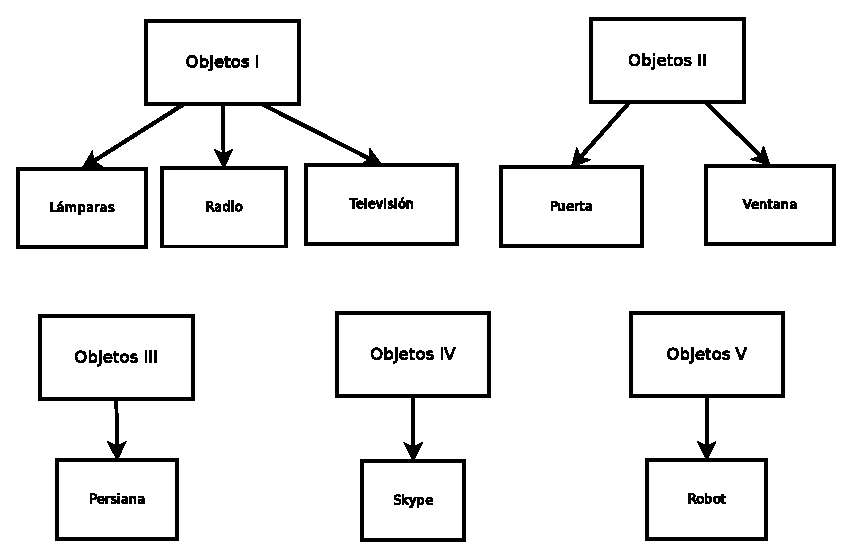
\includegraphics{Esquema_objetos}
  \caption{Clasificación de los objetos para la gramática (aquí también
    se pueden poner acrónimos como \acs{ETTS} y símbolos como \ac{xidet})}
  \label{fig:fig_clobj}
\end{figure}


\subsection{Definición y uso de acrónimos (aquí también
  se pueden poner acrónimos como \acs{ETTS})}
\label{sec:uso-de-acronimos}

El uso del paquete \texttt{glossaries} permite definir los acrónimos y
el sistema automáticamente gestiona su inclusión completa la primera vez
que se usa. Los acrónimos de ejemplo están en el fichero
\texttt{acronyms/defacronymsgl.tex} (con opciones adicionales de
configuración en \texttt{acronyms/acronymsgl.tex}).

Así, si nos referimos a \ac{ETTS} o bien a \ac{EMODB},
veremos como aparecen expandidas la primera vez. A partir de ahí, sólo
se usará el acrónimo como puede verse al volver a hablar de \ac{ETTS} y
\ac{EMODB}.

Tiene también soporte para resetear todos los acrónimos como si no
estuvieran usados. Vuelvo a incluir el párrafo anterior tras un reset
(que se hace con un \texttt{\textbackslash{}glsresetall[acronym]}):

\glsresetall[acronym]

El uso del paquete acronym permite definir los acrónimos y el sistema
automáticamente gestiona su inclusión completa la primera vez que se
usa. Así, si nos referimos a \ac{ETTS} o bien a \ac{EMODB}, veremos como
aparecen expandidas de nuevo (como si fuera la primera vez que se
usan). A partir de ahí, sólo se usará el acrónimo como puede verse al
volver a hablar de \ac{ETTS} y \ac{EMODB}.

Y permite también forzar que se vuelva a citar completo aunque ya se
haya utilizado (con el acrónimo entre paréntesis), como puede verse en
\acl{ETTS} (equivalente a \glsdesc{ETTS} que vale para cualquier
glosario), y también a usar forzosamente el acrónimo. Primero reseteamos
de nuevo.

\glsresetall[acronym]

Y ahora forzamos el acrónimo: \acs{EMODB} (equivalente a
\glsname{EMODB} que vale para cualquier glosario). También podemos
forzar a que lo ponga todo, con \acf{EMODB}.


Podemos seguir definiendo entradas de acrónimos, referirnos a \ac{DBN}
por primera vez, y las siguientes aparecerá como \ac{DBN}.  Pongo ahora
el resto de acrónimos \ac{SQ}, \ac{EIR}, \ac{SIR} y
\ac{ES}. Finalmente los repito para que se vea el efecto: \ac{SQ},
\ac{EIR}, \ac{SIR} y \ac{ES}.

Y gestiona bien los plurales, ponemos el plural como \acp{SOC} la
primera vez, y luego la segunda como \acp{SOC}. Y podemos volver al
singular con \ac{SOC}.


\subsection{Definición y uso de símbolos (aquí también
  se pueden símbolos como \ac{xidet})}
\label{sec:simbolos}

Los símbolos definidos están incluidos en el fichero
\texttt{symbols/defsymbolsgl.tex} (con configuración adicional en
\texttt{symbols/symbolsgl.tex}) y en esta sección mostramos algunos
ejemplos.

El \ac{angstrom} se usa en biología estructural, mientras que el
\ac{ohm} se usa en electrónica. También podemos poner~\ac{xdet}. Y
 


\chapter{Estudio teórico}
\label{cha:estudio-teorico}

\begin{FraseCelebre}
  \begin{Frase}
    Y así, del mucho leer y del poco dormir, se le secó el cerebro de
    manera que vino a perder el juicio\footnote{Tomado de ejemplos del
      proyecto \texis{}.}.
  \end{Frase}
  \begin{Fuente}
    Miguel de Cervantes Saavedra
  \end{Fuente}
\end{FraseCelebre}


\section{Introducción}
\label{sec:introduccion-teoria}

En este capítulo se cuenta tal y tal.

El capítulo se estructura en $n$ apartados\ldots


\section{Estado del Arte}
\label{sec:estadoarte}

En el estado del arte se enumeran los trabajos más relevantes de otros
grupos de investigación. A continuación se muestra un ejemplo del uso de
viñetas que nos proporciona \texttt{itemize}:

\begin{itemize}
\item En el trabajo ..... 
\item En el siguiente trabajo.....
\end{itemize}

O citas en un párrafo real: Sin embargo, hay entornos acústicos donde
las tasas de error conseguidas son todavía demasiado altas. En concreto,
las aplicaciones en las que la captura de la señal de habla se hace
usando micrófonos alejados del locutor (típicamente para distancias
superiores a un metro) muestran una fuerte sensibilidad a los problemas
de reverberación, ruido aditivo y baja relación señal a ruido
(\cite{gelbart02},\cite{kochkin02}). En estos entornos, se ha propuesto
el uso de arrays de micrófonos como un método para mejorar la calidad
del habla capturada \cite{seltzer03}\cite{herbordt05}.

Existen múltiples formas de insertar figuras en Latex. A continuación,
se muestra un ejemplo del uso de \texttt{figure}. Como se puede ver en
la Figura \ref{fig1} también se pueden poner referencias a las figuras
por medio de \texttt{ref} y la etiqueta \texttt{label} de la figura en
particular.

\begin{figure}[h] \centering
  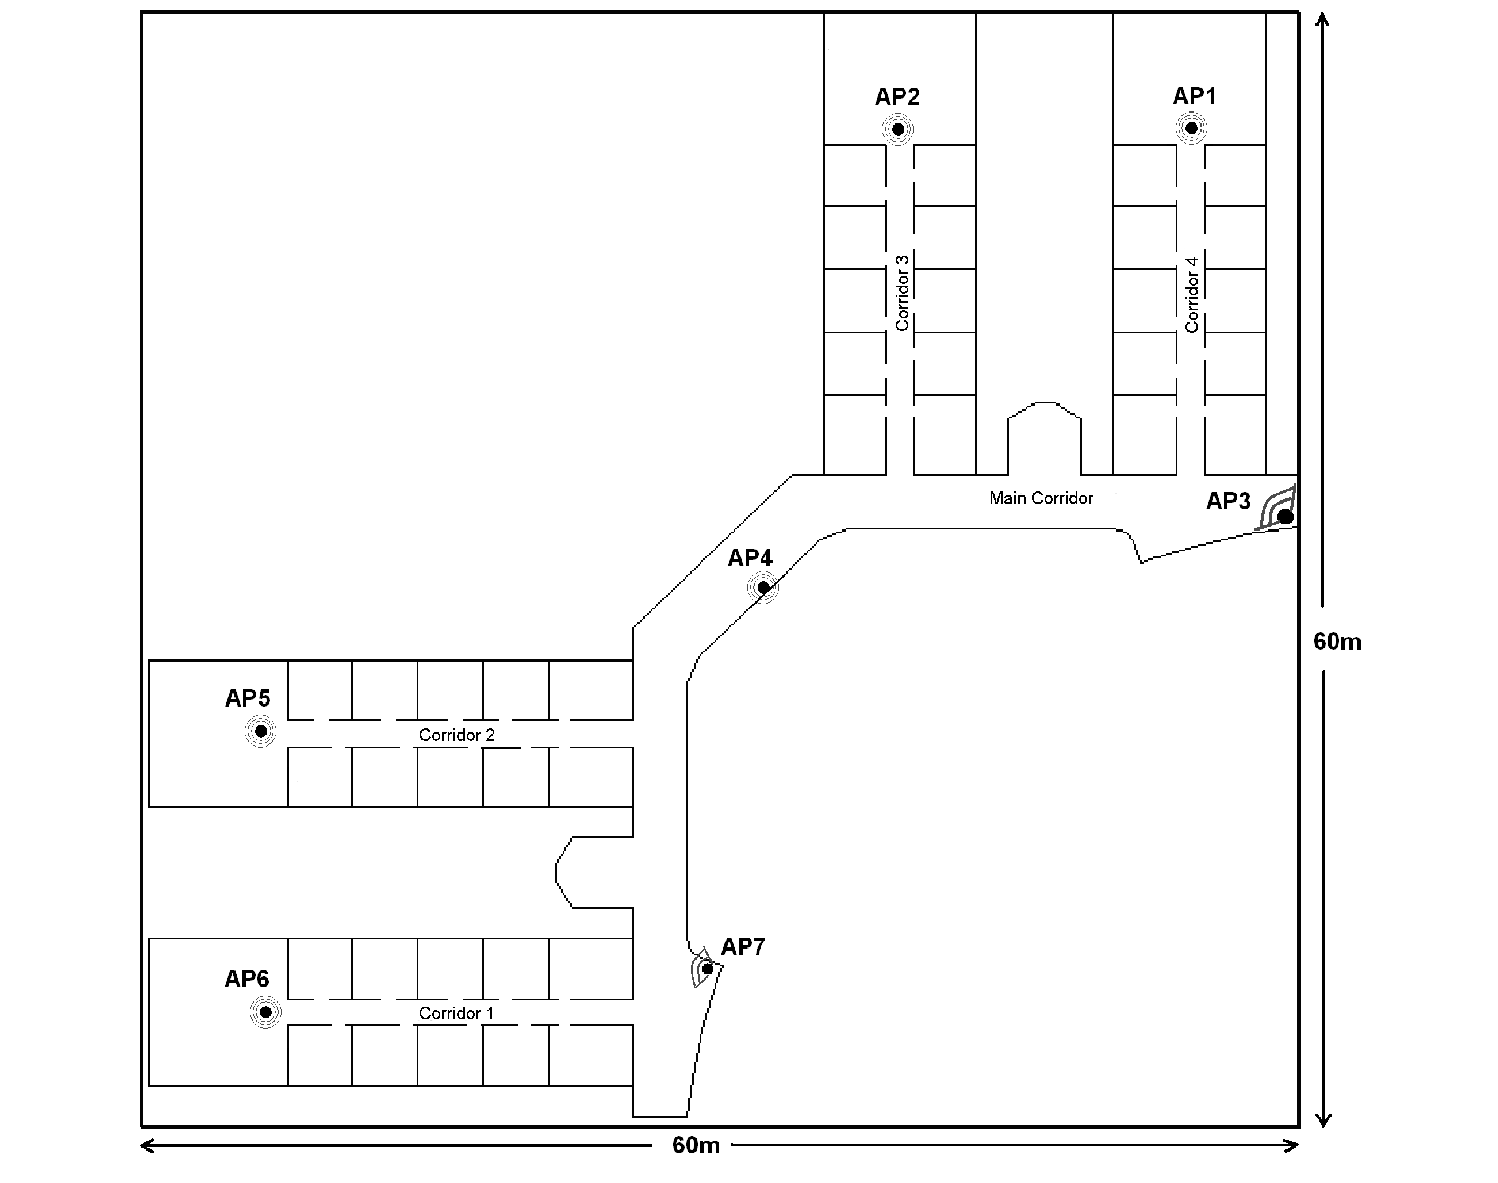
\includegraphics[width=4.7in]{Figure1}
\caption{Departamento de Electrónica.}
  \label{fig1}
\end{figure}

Y ahora un ejemplo en el que ponemos el \texttt{caption} en el lateral:

\begin{SCfigure}
  \centering
  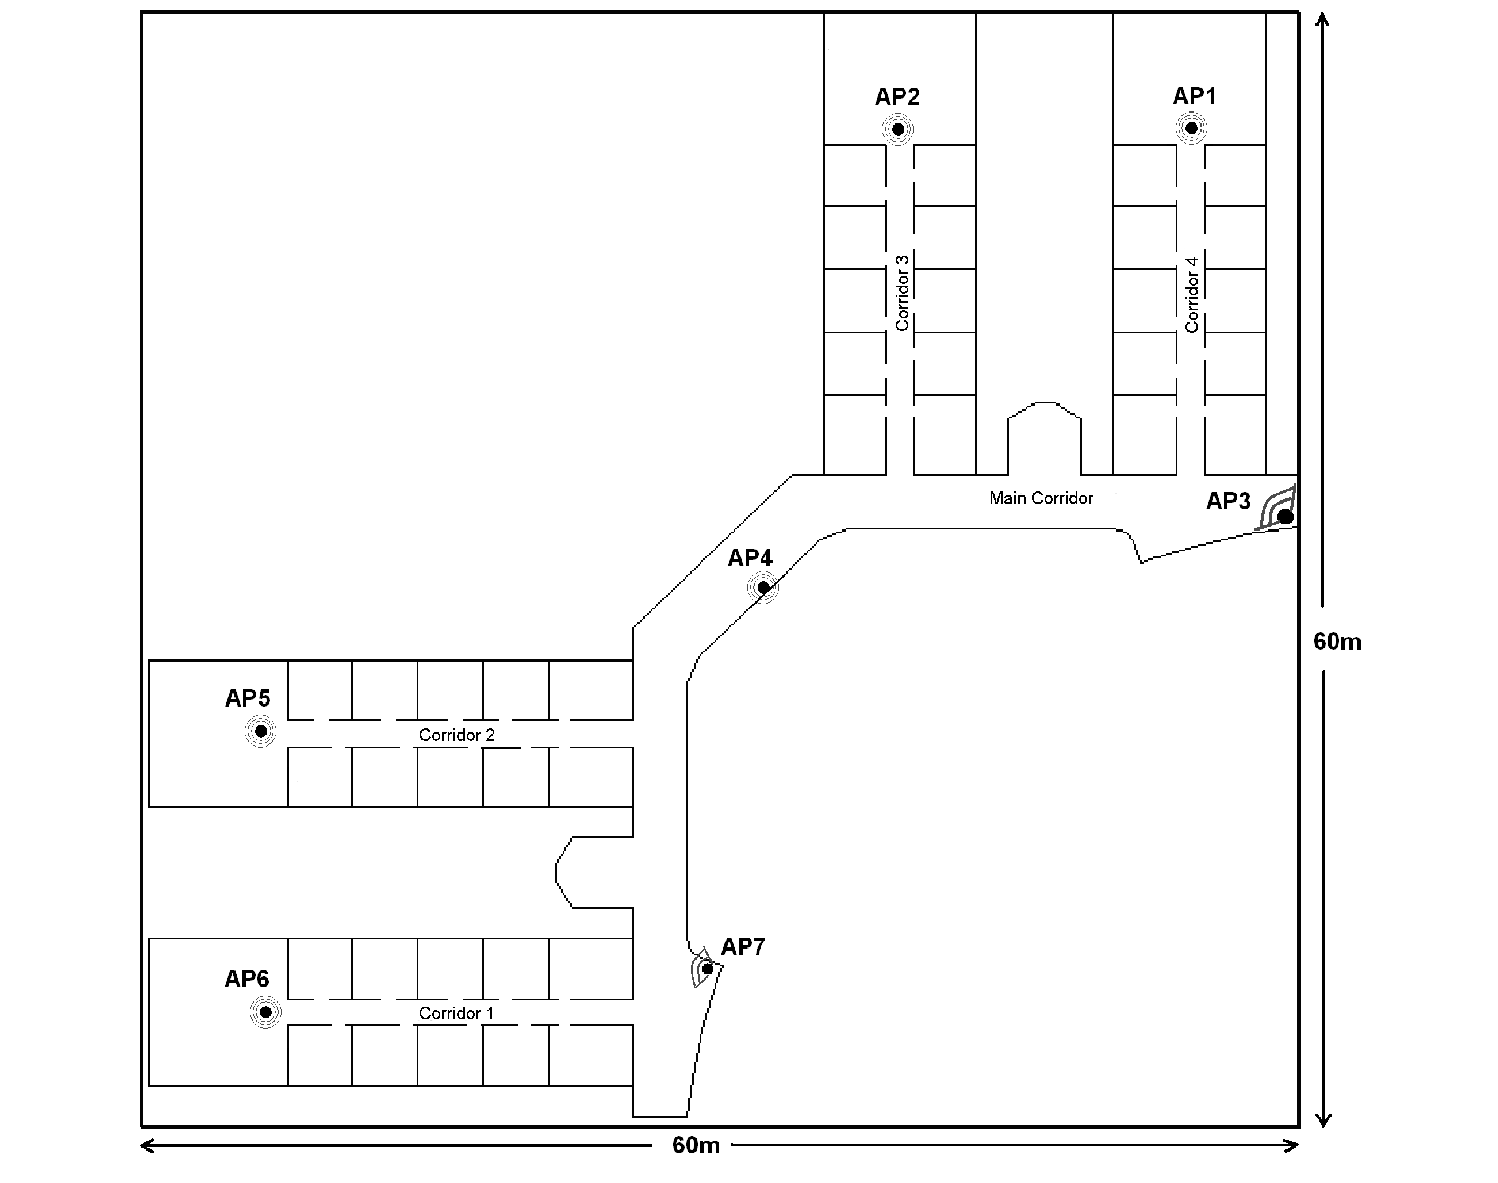
\includegraphics[width=0.5\textwidth]{Figure1}
  \caption{Departamento de Electrónica en el lateral.}
\end{SCfigure}



\section{Técnicas utilizadas}
\label{sec:tecnicas-utilizadas}

Aquí vamos a probar todos los niveles de sección disponibles, para
evaluar la asignación de \texttt{tocdepth}...

Blah, blah, blah\ldots


\subsection{Subsección}
\label{sec:subseccion}


\subsubsection{Subsubsección}
\label{sec:subsubseccion}

\paragraph{Paragraph}
\label{sec:paragraph-1}


\subparagraph{Subparagraph}
\label{sec:subparagraph}



\section{Conclusiones}
\label{sec:conclusiones-teoria}

Blah, blah, blah\ldots

 


\chapter{Desarrollo}
\label{cha:desarrollo}


\begin{FraseCelebre}
  \begin{Frase}
    A fuerza de construir bien, se llega a buen
    arquitecto\footnote{Tomado de ejemplos del proyecto \texis{}.}.
  \end{Frase}
  \begin{Fuente}
    Aristóteles
  \end{Fuente}
\end{FraseCelebre}

\section{Introducción}
\label{sec:introduccion-desarrollo}

En este capítulo se incluirá la descripción del desarrollo del trabajo.

El capítulo se estructura en n apartados:...


\section{Desarrollo del sistema de experimentación}
\label{sec:desarr-del-sist}

Blah, blah, blah\ldots


\section{Planteamiento matemático}
\label{sec:libr-desarr}

También resulta útil poder introducir ecuaciones que se encuentran tanto
en línea con el texto (como por ejemplo $\sigma=0.75$), como en un
párrafo aparte (como en la ecuación \ref{eq1}). Al igual que ocurre con
las figuras, también se pueden referenciar las ecuaciones.

\begin{equation}
  \label{eq1}
  p[q_t=\sigma_t|q_{t-1}=\sigma_{t-1}]
\end{equation}

\section{Conclusiones}
\label{sec:conclusiones-desarrollo}

Blah, blah, blah\ldots



 


\chapter{Resultados}
\label{cha:resultados}


\begin{FraseCelebre}
  \begin{Frase}
Rem tene, verba sequentur (Si dominas el tema, las palabras vendrán
    solas)\footnote{Tomado de ejemplos del proyecto \texis{}.}.
  \end{Frase}
  \begin{Fuente}
Catón el Viejo
  \end{Fuente}
\end{FraseCelebre}

\section{Introducción}
\label{sec:introduccion-resultados}

En este capítulo se introducirán los resultados más relevantes del
trabajo. 

La estructura del capítulo es\ldots


\section{Entorno experimental}
\label{sec:entorno-experimental}

Blah, blah, blah.


\subsection{Bases de datos utilizadas}
\label{sec:bases-de-datos-1}

Blah, blah, blah.


\subsection{Métricas de calidad}
\label{sec:metricas-de-calidad}

Blah, blah, blah.

En la tabla\ref{pruebaCalc2LaTeX} pongo un ejemplo del uso del conversor
de libreoffice a \LaTeX{} (cortesía de Roberto Chamorro). Para usarlo
tienes que importar la macro que encontrarás en el directorio
\texttt{Tools/calc2latex//calc2latex\_024\_eur\_latex}\footnote{Para
  ello sigue el proceso de importación que se describe en
  \url{http://ask.libreoffice.org/en/question/35598/where-are-lo-basic-macros-stored/},
  importando Cals
  y cuando ejecutes la macro hazlo por el punto de entrada
  \texttt{Main}, después de seleccionar el rango de celdas de la tabla.}

\begin{table}[htbp]
\caption{Caption de prueba de tabla LaTeX convertida desde
  \texttt{libreoffice} con la macro \texttt{calc2latex}.}
\begin{center}
\begin{tabular}{|l|r|r|r|}
\hline
 & \multicolumn{1}{l|}{System A} & \multicolumn{1}{l|}{System B} & \multicolumn{1}{l|}{System C} \\ \hline
FA rate & 10,00\% & 5,00\% & 2,00\% \\ \hline
TA rate & 90,00\% & 85,00\% & 75,00\% \\ \hline
\end{tabular}
\end{center}
\label{pruebaCalc2LaTeX}
\end{table}

 

\subsection{Estrategia y metodología de experimentación}
\label{sec:estr-y-metod}

Blah, blah, blah.


\section{Resultados experimentales}
\label{sec:result-experim}

A continuación, se muestra un ejemplo de tabla simple (ver tabla \ref{table1}).

\begin{table}
\renewcommand{\arraystretch}{1.3}
  \caption{Comparativa.}
  \label{table1}
  \begin{center}
\begin{tabular}{|c|c|c|}
      \hline
      Method & Training Time & Man-Work (\%)\\
      \hline
      Propagation model & $<$ 30 sec & 5\\
      \hline
      Manual & 9 h 30 min & 24\\
      \hline
      Automatic & 2 h & 10 8\\
      \hline
    \end{tabular}
  \end{center}
\end{table}

Cuando las tablas ocupan más de un página se debe utilizar un tipo
especial de tablas denominado \texttt{longtable}. A continuación, se
muestra un ejemplo del mismo (ver tabla \ref{table2}).

\begin{center}
	\begin{longtable}{|c|c|c|c|}
    \caption[Resultados de la correlación cruzada.]{Resultados de la correlación cruzada.} \label{table2} \\
    
    \hline \multicolumn{1}{|c|}{\textbf{Posición Real}} & \multicolumn{1}{c|}{\textbf{Posición estimada}} & \multicolumn{1}{c|}{\textbf{Coef. Correlación}} & \multicolumn{1}{c|}{\textbf{Acierto/Fallo}} \\ \hline 
    \endfirsthead
    
    \multicolumn{4}{c}{{\bfseries \tablename\ \thetable{} -- continúa en la página anterior}} \\
    \hline \multicolumn{1}{|c|}{\textbf{Posición Real}} & \multicolumn{1}{c|}{\textbf{Posición estimada}} & \multicolumn{1}{c|}{\textbf{Coef. Correlación}} & \multicolumn{1}{c|}{\textbf{Acierto/Fallo}} \\ \hline 
    \endhead
    
    \hline \multicolumn{4}{|r|}{{Continúa en la página siguiente}} \\ \hline
    \endfoot

    \hline \hline
    \endlastfoot
    
    \hline	2P0	&	2P0	&	0,004954	&	A	\\
    \hline	2P1	&	2P4	&	0,005752	&	F	\\
    \hline	2P2	&	2P2	&	0,005461	&	A	\\
    \hline	2P3	&	2P0	&	0,004634	&	F	\\
    \hline	2P5	&	2P4	&	0,005991	&	F	\\
    \hline	2P6	&	2P16	&	0,004410	&	F	\\
    \hline	2P7	&	3P9	&	0,008038	&	F	\\
    \hline	2P8	&	3P9	&	0,003753	&	F	\\
    \hline	2P9	&	2P7	&	0,004908	&	F	\\
    \hline	2P10	&	2P10	&	0,007273	&	A	\\
    \hline	2P14	&	2P16	&	0,006485	&	F	\\
    \hline	2P15	&	2P15	&	0,004932	&	A	\\
    \hline	2P16	&	2P16	&	0,006237	&	A	\\
    \hline	2P17	&	2P15	&	0,005110	&	F	\\
    \hline	2P18	&	3P18	&	0,006235	&	F	\\
    \hline	2P19	&	3P18	&	0,004827	&	F	\\
    \hline	2P20	&	2P20	&	0,006877	&	A	\\
    \hline	2P22	&	3P18	&	0,003048	&	F	\\
    \hline	2P24	&	2P24	&	0,006833	&	A	\\
    \hline	2P25	&	2P25	&	0,004875	&	A	\\
    \hline	2P26	&	2P31	&	0,005511	&	F	\\
    \hline	2P27	&	2P28	&	0,004590	&	F	\\
    \hline	2P30	&	2P31	&	0,005576	&	F	\\
    \hline	2P31	&	2P31	&	0,007213	&	A	\\
    \hline	2P32	&	2P35	&	0,003340	&	F	\\
    \hline	2P34	&	2P34	&	0,004128	&	A	\\
    \hline	2P36	&	2P35	&	0,003329	&	F	\\
    \hline	2P37	&	2P37	&	0,003468	&	A	\\
    \hline	2P39	&	2P38	&	0,002577	&	F	\\
    \hline	2P40	&	2P43	&	0,004303	&	F	\\
    \hline	2P41	&	2P41	&	0,001573	&	A	\\
    \hline	2P42	&	2P41	&	0,000846	&	F	\\
    \hline	2P44	&	2P44	&	0,002732	&	A	\\
    \hline	2P45	&	23P45	&	0,001958	&	F	\\
    \hline	2P47	&	2P34	&	0,002869	&	F	\\
    \hline	2P48	&	2P43	&	0,004569	&	F	\\
    \hline	2P49	&	3P51	&	0,001374	&	F	\\
    \hline	2P50	&	2P34	&	0,002274	&	F	\\
    \hline	2P51	&	2P63	&	0,003931	&	F	\\
    \hline	2P52	&	2P55	&	0,003537	&	F	\\
    \hline	2P53	&	3P56	&	0,003126	&	F	\\
    \hline	2P54	&	2P67	&	0,005560	&	F	\\
    \hline	2P56	&	2P55	&	0,002817	&	F	\\
    \hline	2P57	&	2P67	&	0,006168	&	F	\\
    \hline	2P58	&	2P58	&	0,005278	&	A	\\
    \hline	2P60	&	3P66	&	0,004966	&	F	\\
    \hline	2P61	&	3P61	&	0,004748	&	A	\\
    \hline	2P64	&	2P67	&	0,005342	&	F	\\
    \hline	2P66	&	2P4	&	0,004172	&	F	\\
    \hline	2P67	&	2P67	&	0,005706	&	A	\\
    \hline	3P0	&	3P0	&	0,003674	&	A	\\
    \hline	3P61	&	2P61	&	0,003263	&	F	\\
    \hline	3P64	&	2P67	&	0,003484	&	F	\\
    \hline	3P65	&	2P67	&	0,002975	&	F	\\
    \hline	3P66	&	2P58	&	0,005029	&	F	\\
    \hline	3P67	&	3P67	&	0,003714	&	A	\\
	\end{longtable}
\end{center}





En algunas ocasiones, también resulta útil emplear el entorno
\texttt{subfigure} para añadir múltiples imágenes dentro de la misma
figura. A continuación, se muestra un ejemplo del uso en la figura
\ref{fig:fig3}. También se pueden referenciar las sub-figuras de forma
individual, por ejemplo la sub-figura \ref{fig:fig3b} (usando un método
de cita), o bien la sub-figura \ref{fig:fig3}.\subref{fig:fig3b} (usando
otro alternativo).

\begin{figure}
  \centering
  \begin{subfigure}[b]{0.3\textwidth}
    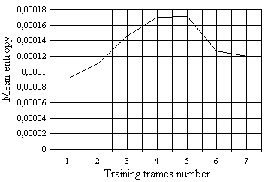
\includegraphics[width=\textwidth]{Figure2}
    \caption{Mean Entropy.}
    \label{fig:fig3a}
  \end{subfigure}~ \begin{subfigure}[b]{0.3\textwidth}
    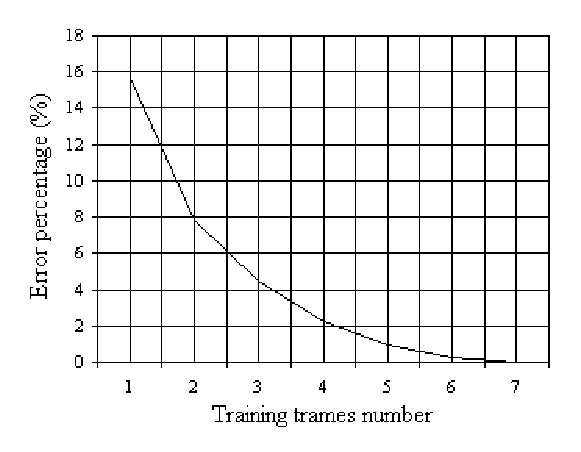
\includegraphics[width=\textwidth]{Figure3}
    \caption{Error Percentage.}
    \label{fig:fig3b}
  \end{subfigure}
  \caption{Optimal trames number in the training data set.}
  \label{fig:fig3}
\end{figure}

La figura~\ref{fig:LIdiapRoom} muestra otro ejemplo con referencias a
las subfigures en el caption principal. 

\begin{figure}
  \centering
  \begin{subfigure}[b]{0.30\textwidth}
    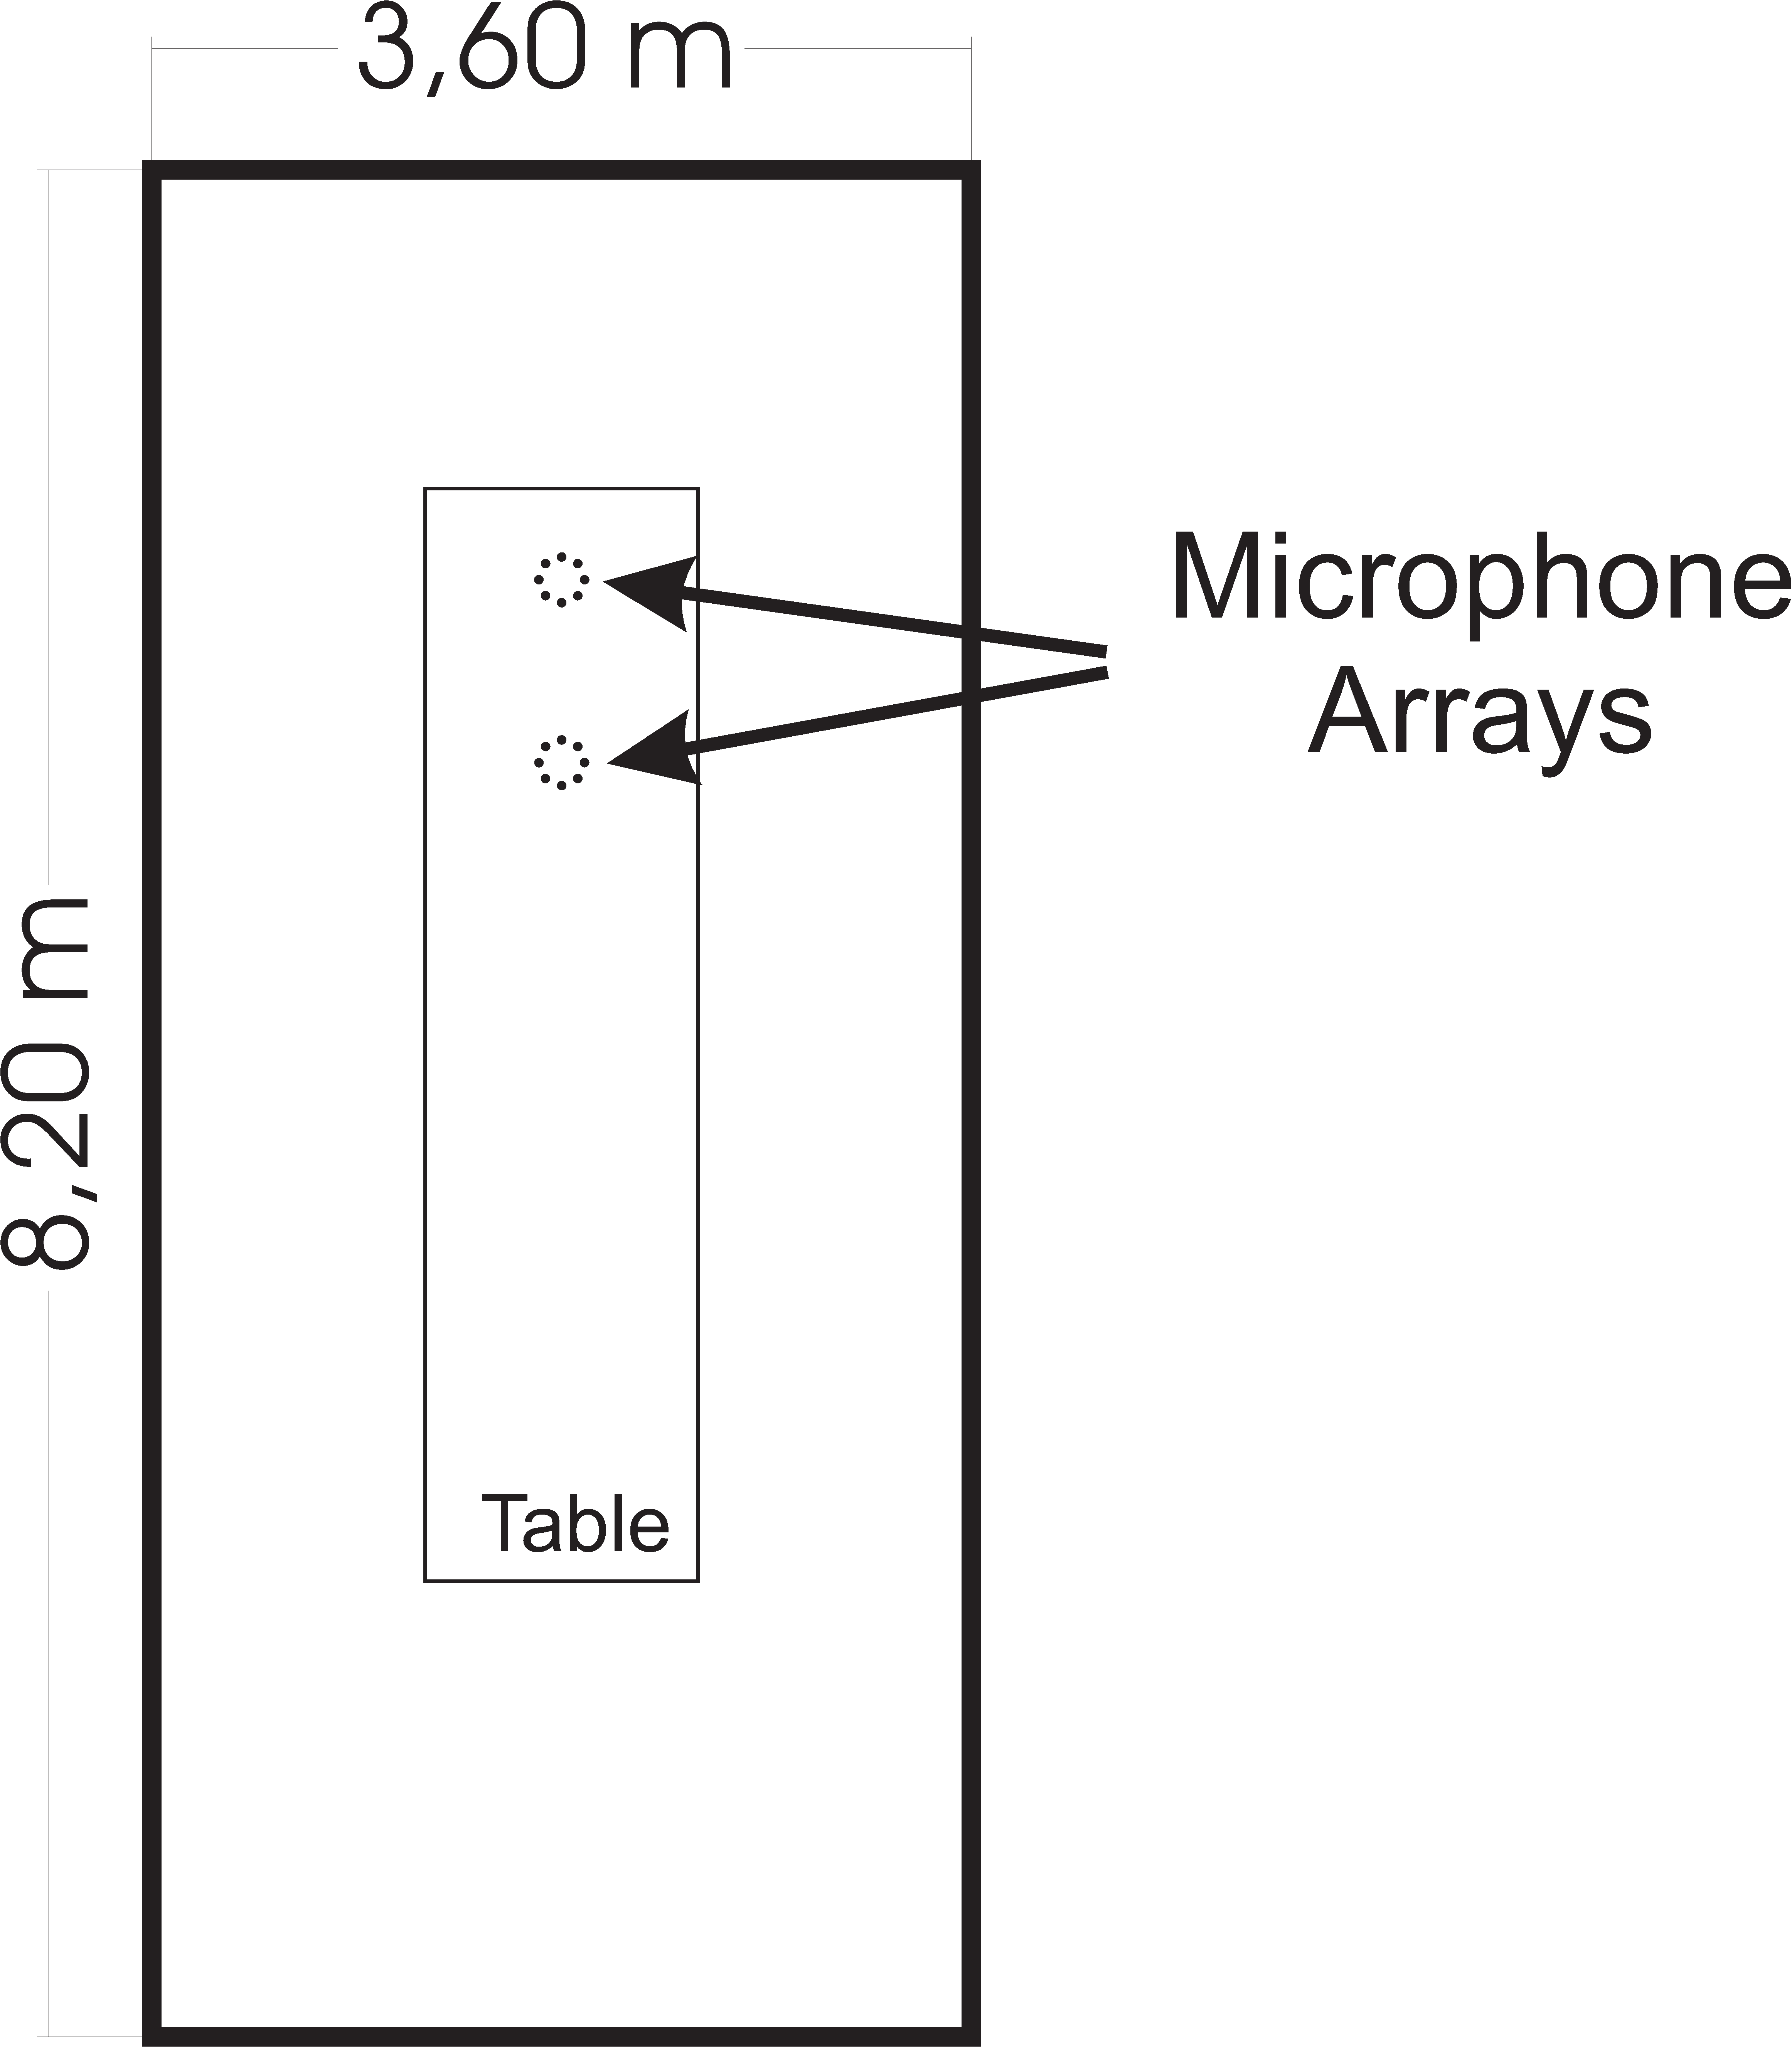
\includegraphics[width=\textwidth]{roomlayout2}
    \caption{}
    \label{fig:RoomLayout}
  \end{subfigure}\qquad \qquad \begin{subfigure}[b]{0.425\textwidth}
    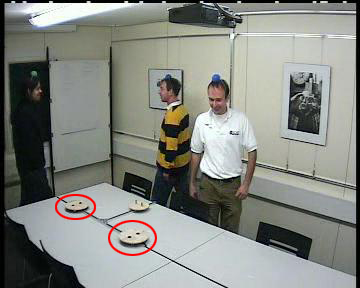
\includegraphics[width=\textwidth]{idiap-seq45-cam2.jpg}
    \caption{}
    \label{fig:RoomPicture}
  \end{subfigure}
  \caption{Idiap Smart Meeting Room for AV16.3 recordings.
    (\protect\subref{fig:RoomLayout}) Room layout showing the centered
    table, and the microphones arranged in two circular arrays.
    (\protect\subref{fig:RoomPicture}) Sample of recorded video frame
    showing the arrays area. \vspace{-0.3cm}}
  \label{fig:LIdiapRoom}
\end{figure}

Os incluimos a continuación un
párrafo de un artículo en el que hacemos referencia a varias figuras y
subfiguras: 

\emph{The IDIAP Meeting Room (shown in figure~\ref{fig:LIdiapRoom}) is a $8.2m
\times 3.6m \times 2.4m$ rectangular space containing a centrally
located $4.8m \times 1.2m$ rectangular table, on top of which two
circular microphone arrays of $10 cm$ radius are located, each of them
composed by 8 microphones. The centers of the two arrays are separated
by $80 cm$ and the origin of coordinates is located in the middle point
between the two arrays. The arrays can be also seen in
figures~\ref{fig:simureal_positions}.\subref{fig:Simulated_positions},
~\ref{fig:simureal_positions}.\subref{fig:real_positions_short}, and
~\ref{fig:simureal_positions}.\subref{fig:real_positions_long}, in which
only the relevant section of the room is displayed, each one showing
different scenarios that were used in the experiments. A detailed
description of the meeting room can be found in~\cite{moore2002}.}

\begin{figure}
  \centering
  \begin{subfigure}[t]{0.3\textwidth}
    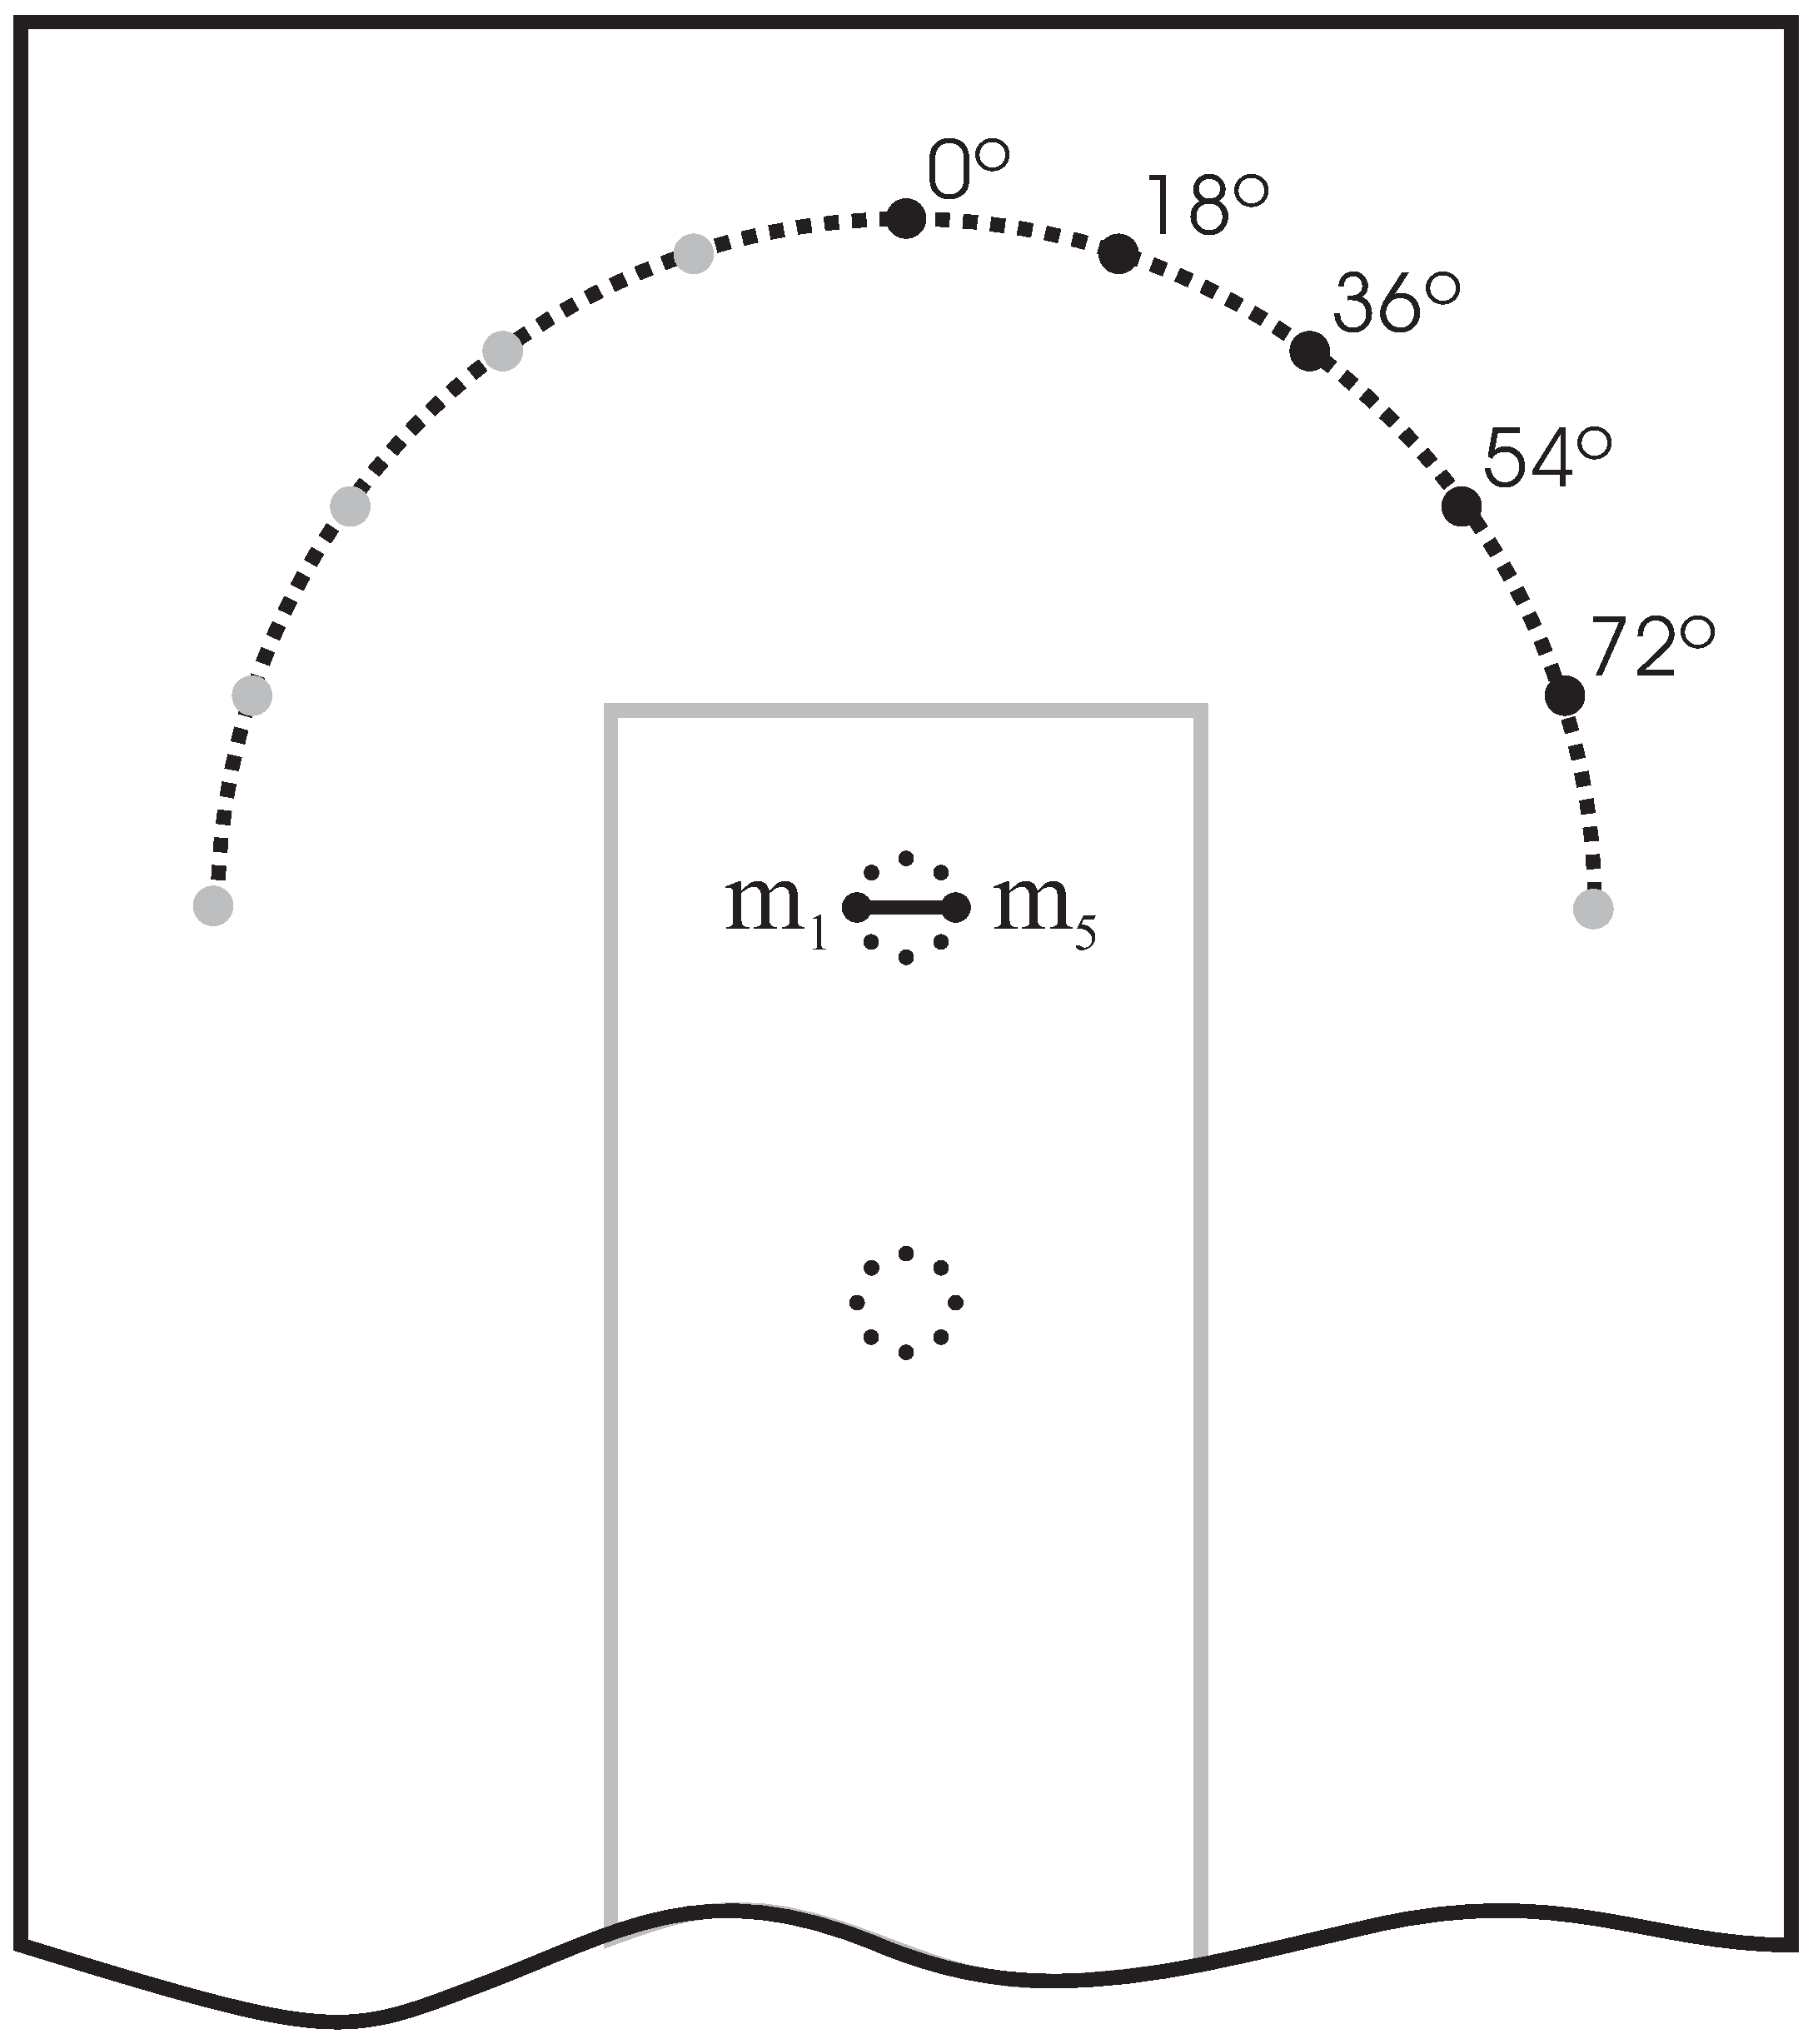
\includegraphics[width=\textwidth]{angular2-short-improved}
    \caption{For validation\\with simulated data.}
    \label{fig:Simulated_positions}
  \end{subfigure}
~\begin{subfigure}[t]{0.3\textwidth}
    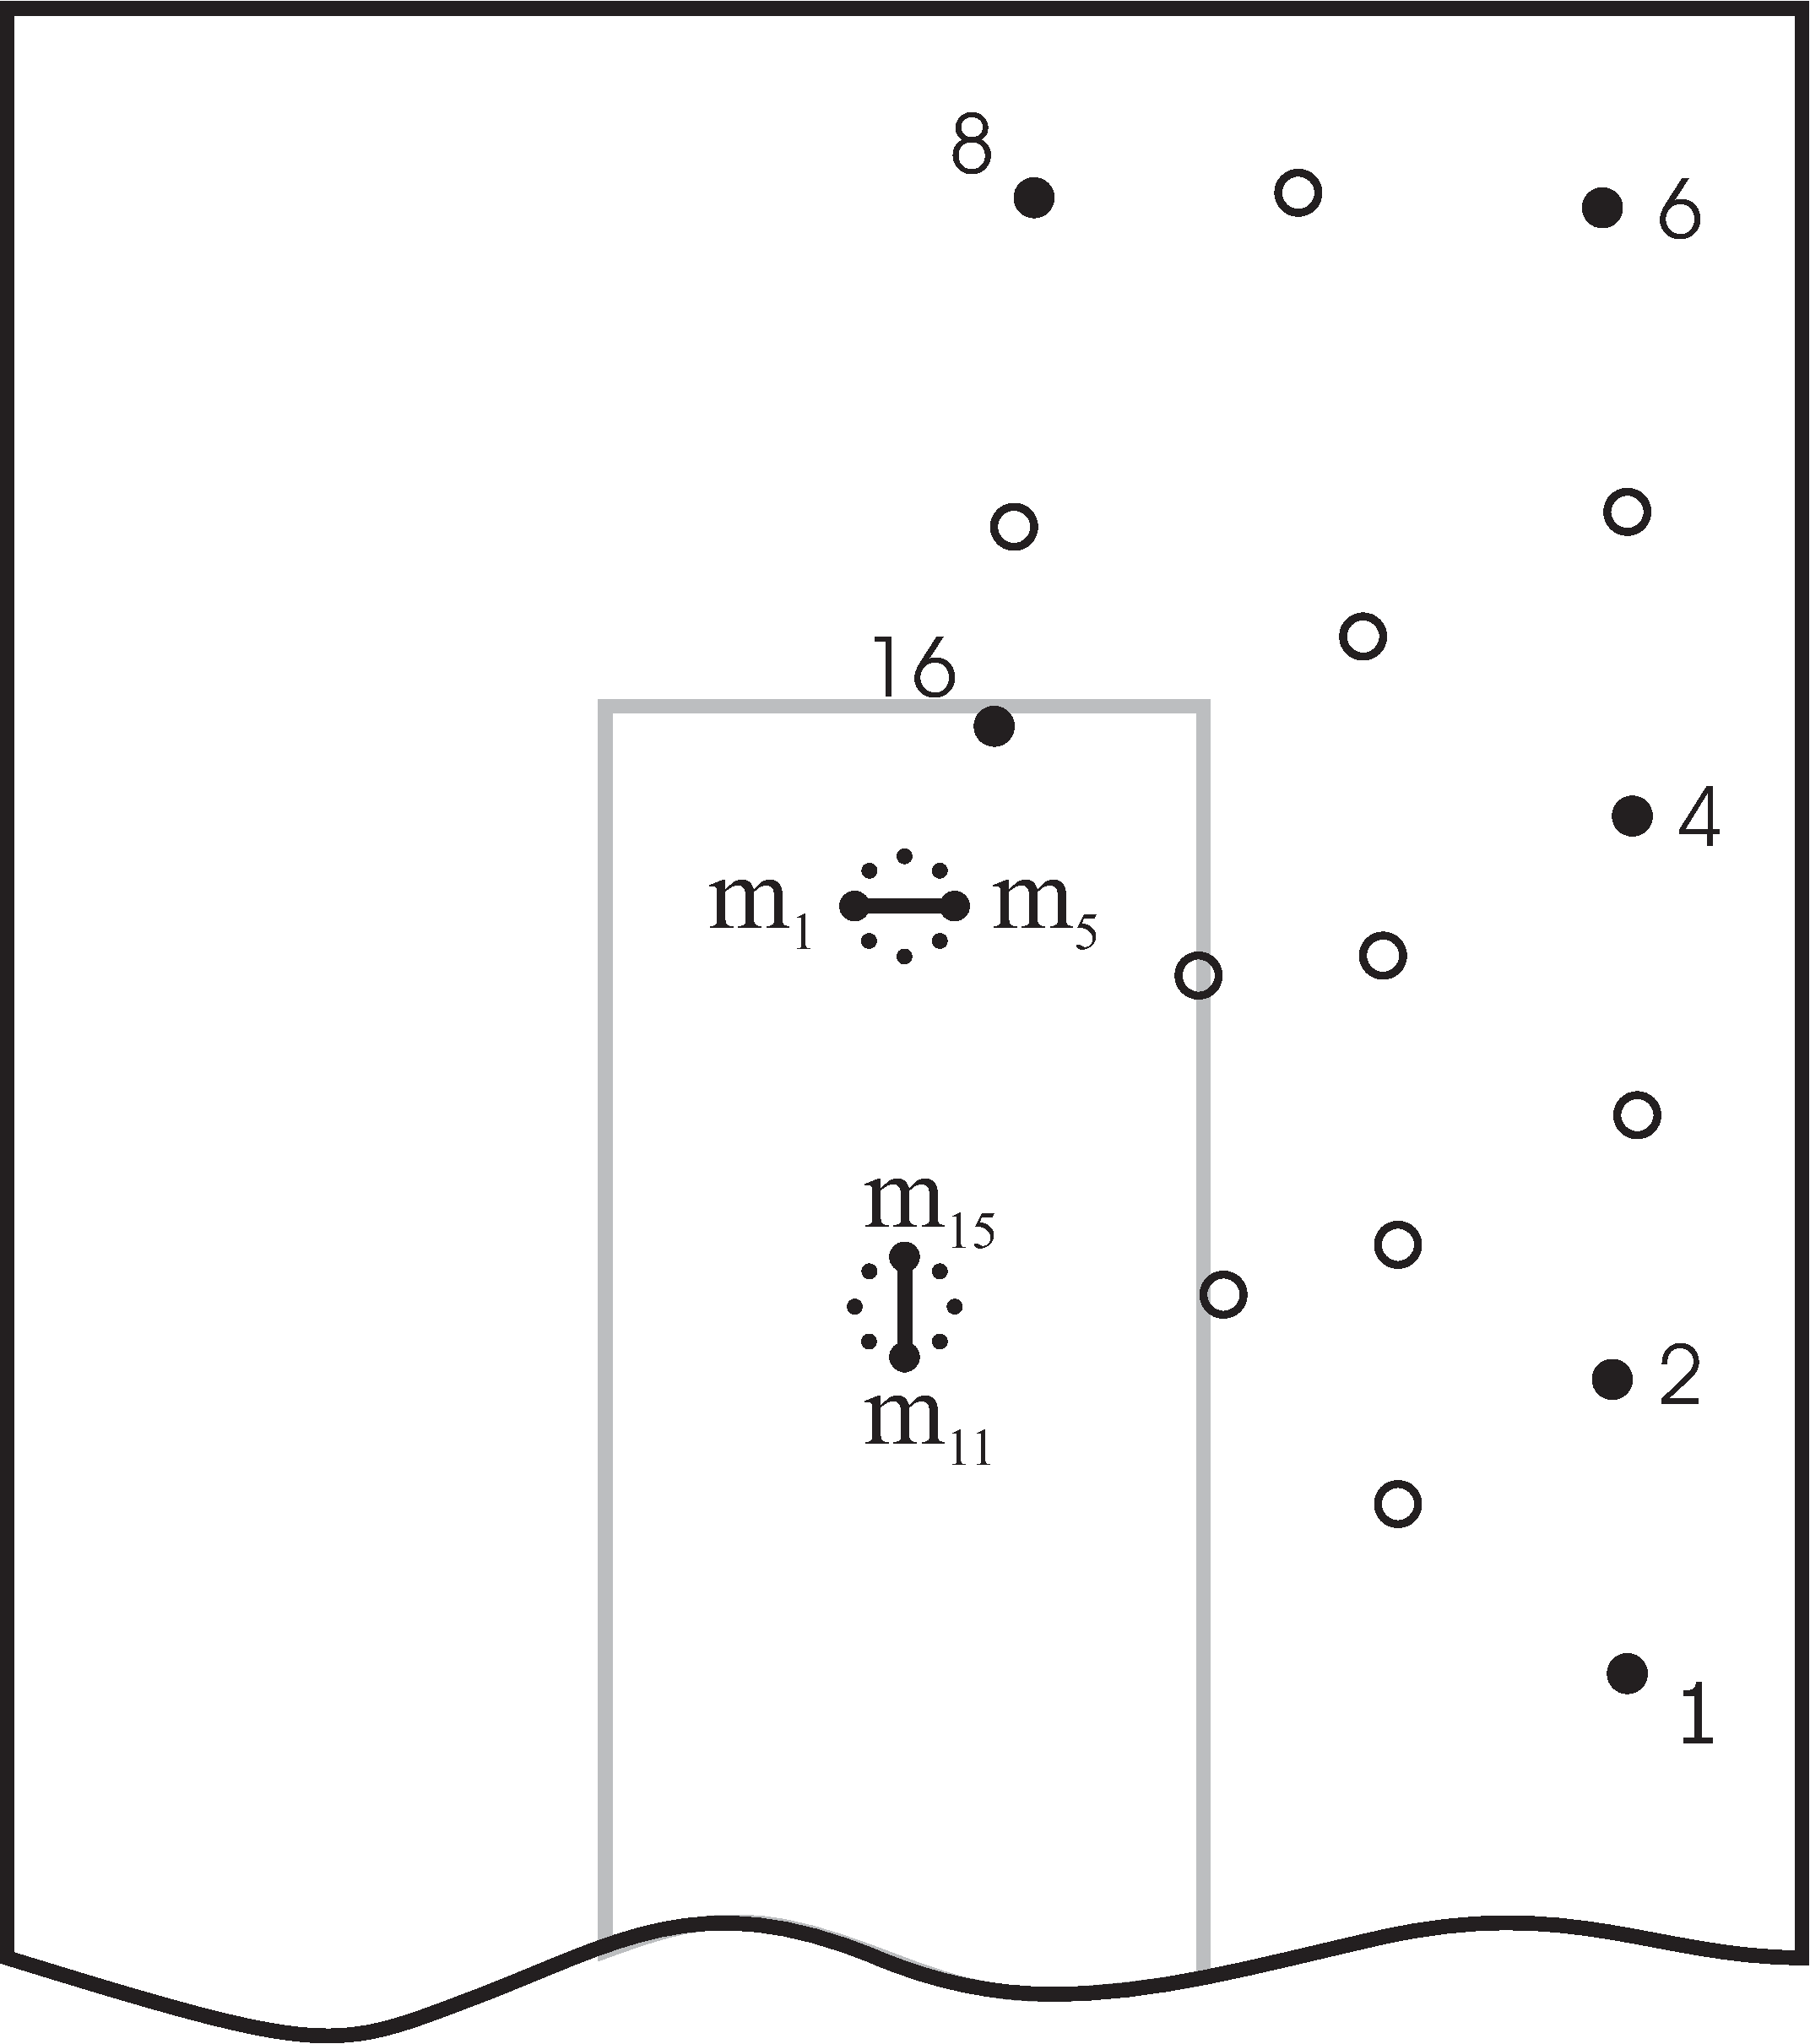
\includegraphics[width=\textwidth]{positions1-short-improved}
    \caption{For validation\\with real data and microphone pairs with $20~cm$ spacing.}
    \label{fig:real_positions_short}
  \end{subfigure}
  ~
  \begin{subfigure}[t]{0.3\textwidth}
    
\includegraphics[width=\textwidth]{positions2-short-improved}
    \caption{For validation\\with real data and microphone pairs with
      $82.46~cm$ spacing.}
    \label{fig:real_positions_long}
  \end{subfigure}
  \caption{Geometrical details for the experiments carried out. Only the
    relevant section of the room is shown, and microphone pairs are
    connected by solid lines.}
  \label{fig:simureal_positions}
\end{figure}

En la figura~\ref{fig:Sim_angles} mostramos un ejemplo de varias
figuras organizadas de forma un poco más complejo.

\begin{figure}
  \centering
  \begin{subfigure}[b]{0.3\textwidth}
    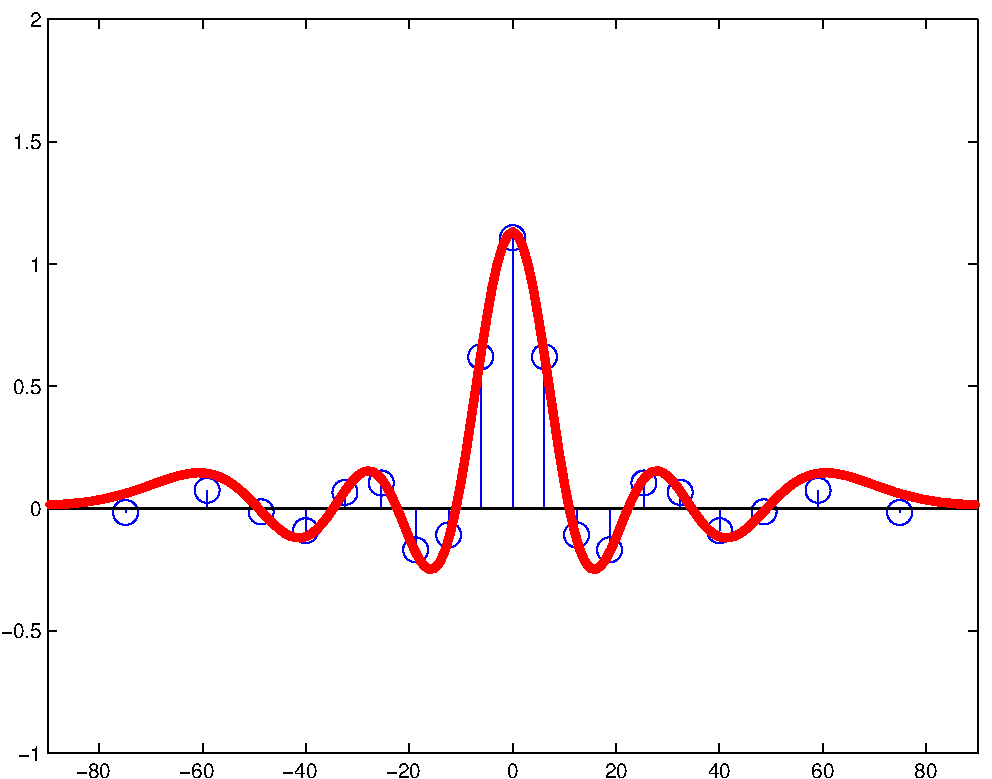
\includegraphics[width=\textwidth]{Sim_seg025_ang090}
    \caption{$0^{\circ}$}
    \label{fig:Sim_ang090}
  \end{subfigure}


  \begin{subfigure}[b]{0.3\textwidth}
    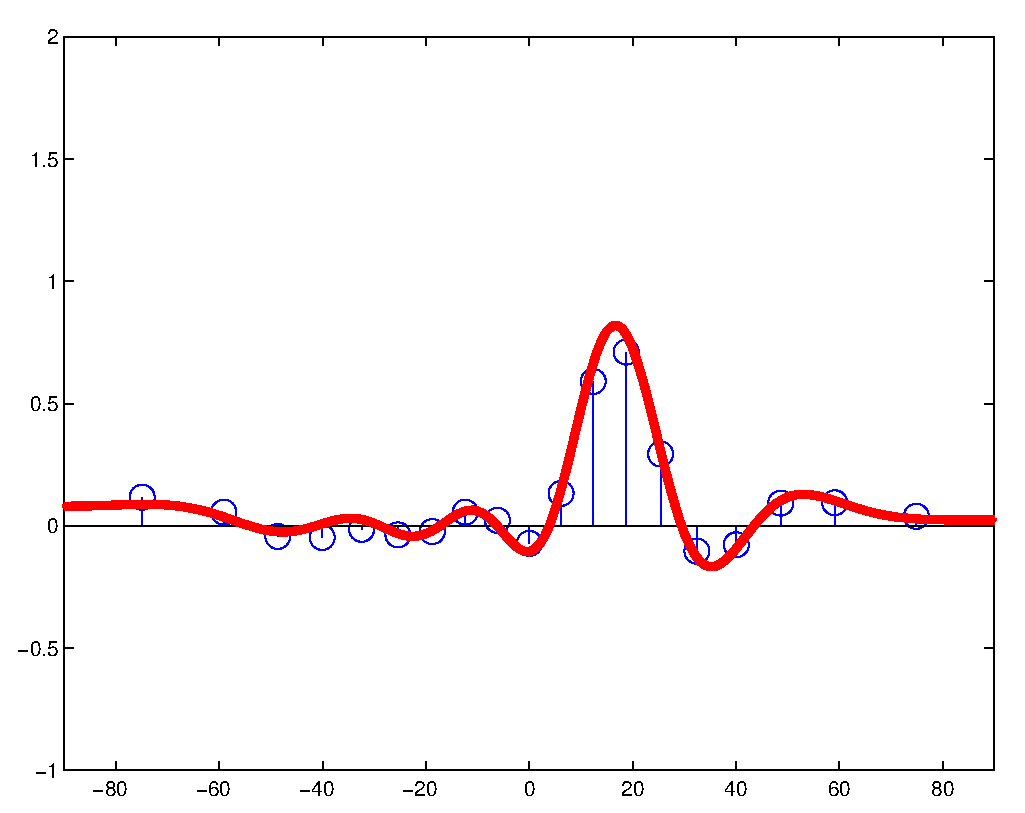
\includegraphics[width=\textwidth]{Sim_seg025_ang108}
    \caption{$18^{\circ}$}
    \label{fig:Sim_ang108}
  \end{subfigure}
\begin{subfigure}[b]{0.3\textwidth}
    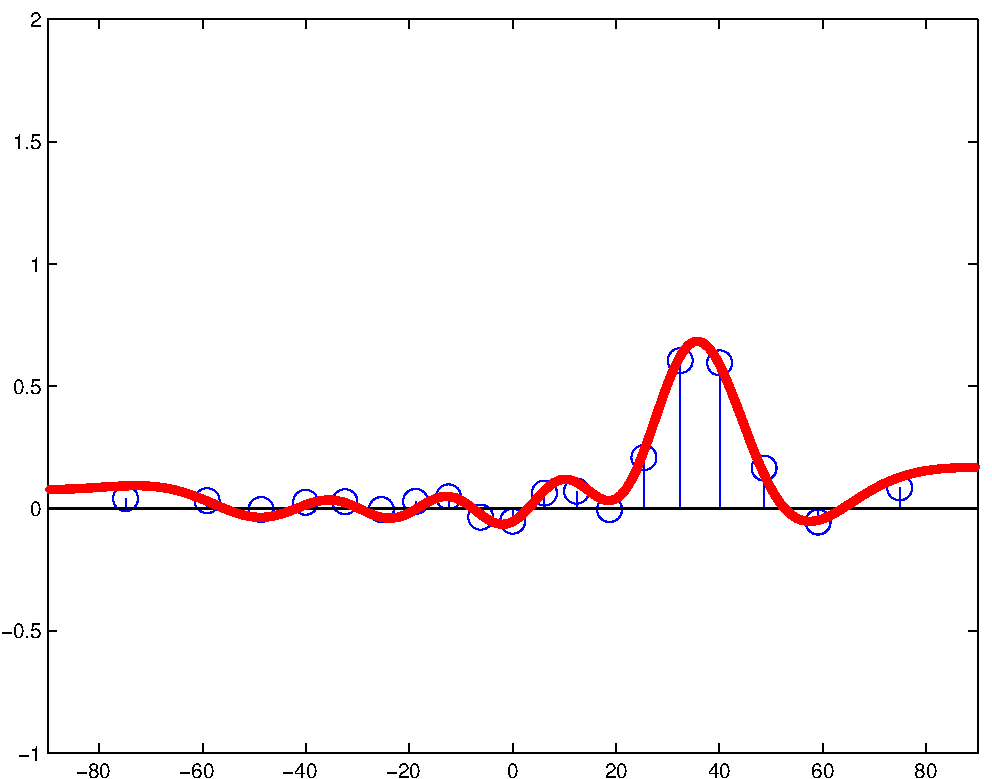
\includegraphics[width=\textwidth]{Sim_seg025_ang126}
    \caption{$36^{\circ}$}
    \label{fig:Sim_ang126}
  \end{subfigure}
\begin{subfigure}[b]{0.3\textwidth}
    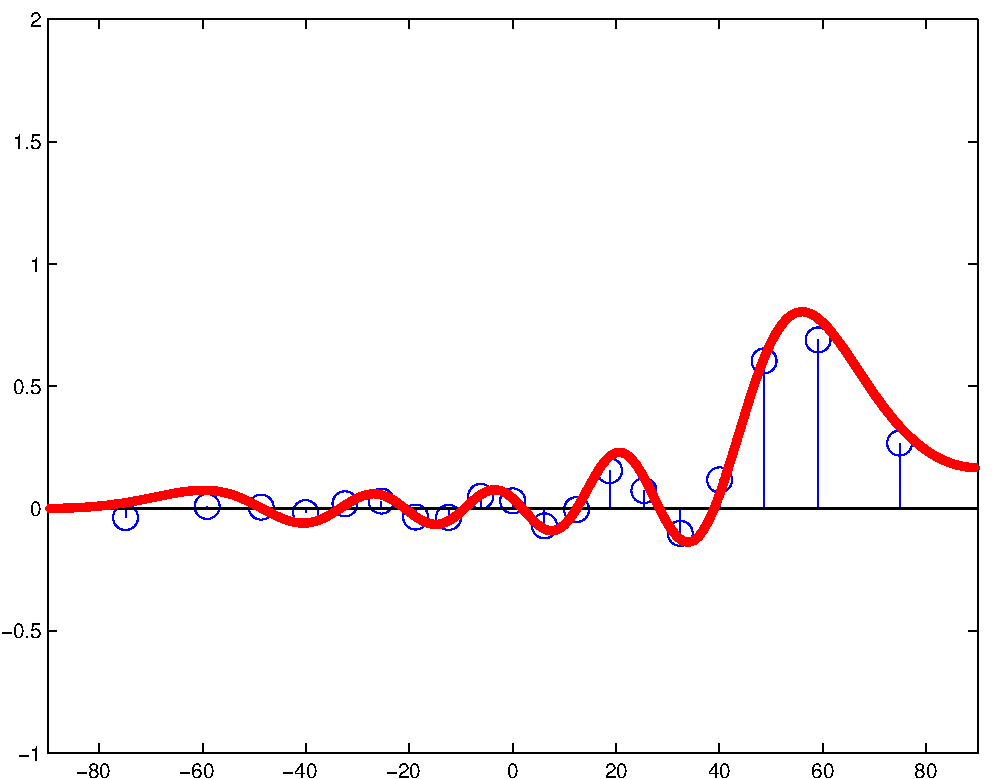
\includegraphics[width=\textwidth]{Sim_seg025_ang144}
    \caption{$54^{\circ}$}
    \label{fig:Sim_ang144}
  \end{subfigure}


  \begin{subfigure}[b]{0.3\textwidth}
    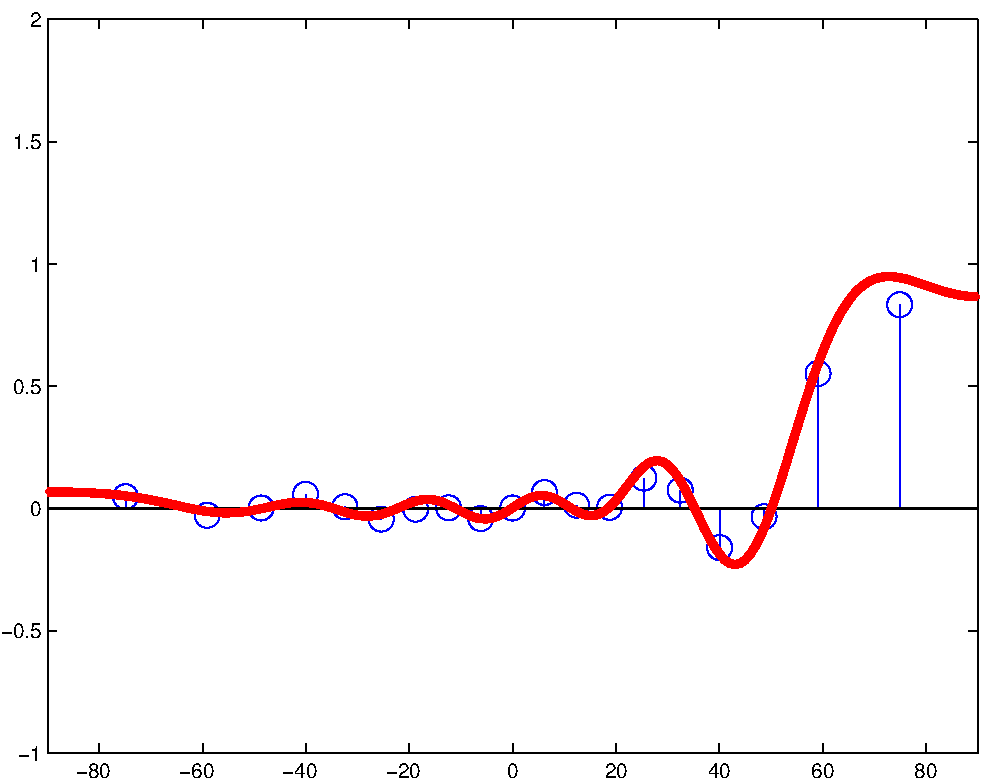
\includegraphics[width=\textwidth]{Sim_seg025_ang162}
    \caption{$72^{\circ}$}
    \label{fig:Sim_ang162}
  \end{subfigure}

  \caption{Comparison between the steered power response generated
    by the model (solid line) and that calculated using simulated
    waveforms in the AV16.3 environment (stems). Results for the
    speaker in given angles and the array steered from -90º to
    +90º are shown.}
  \label{fig:Sim_angles}
\end{figure}

También es posible incluir el código de una figura en un fichero
\texttt{.tex} independiente (para hacer más legible el código del
documento principal). Un ejemplo lo tenéis a continuación, incluyendo el
texto en inglés del documento original:

\emph{Figure~\ref{fig:SRPvsPatternSelected} includes the results of the
comparison, for several speaker positions (1, 2, 4, 6, 8 and 16,
emphasized in
figure~\ref{fig:simureal_positions}.\subref{fig:real_positions_short}),
and selected to provide different acoustic situations, both in terms of
distance and angular position with respect to the arrays. All the
graphics show the acoustic power map (predicted or calculated) for a
regular two-dimensional grid of $10~cm$. The plot is provided from a top
view of the room, spanning the full plan at a height of $61~cm$ above the
microphone arrays (this height was the ground truth one for sequence
01). For each speaker position shown, three graphics are plotted:}

\begin{itemize}
\item \emph{The graphics on the left show the SRP-PHAT acoustic power maps
  generated by the proposed model (for example, the left graphic in
  figure~\ref{fig:SRPvsPatternSelected}.\subref{fig:SRPvsModel_Fo1500_position1}
  for position 1).}
\item \emph{The graphics in the middle show the real SRP-PHAT acoustic power
  maps calculated using the real acoustic waveforms (for example, the
  middle graphic in
  figure~\ref{fig:SRPvsPatternSelected}.\subref{fig:SRPvsModel_Fo1500_position1}
  for position 1), for a single selected frame.}
\item \emph{The graphics on the right show the average real SRP-PHAT acoustic
  power maps, averaging for all the frames in which the user was in the
  given position (for example, the right graphic in
  figure~\ref{fig:SRPvsPatternSelected}.\subref{fig:SRPvsModel_Fo1500_position1}
  for position 1).}
\end{itemize}

\emph{The green point represents the real (ground truth) speaker
position, and the black dots represent the positions of the four
microphones used. The hyperbolic shapes found in the figure are
consistent with the fact that the place of points with equal acoustic
power value, for a given microphone pair, is a hyperbola (in our
two-dimensional case, being a hyperboloid of revolution in the
three-dimensional case).}

\emph{From figure~\ref{fig:SRPvsPatternSelected}, it can clearly be seen that,
again, the predictions closely match the results with real data for the
different acoustic conditions, even when the simulations are using fixed
and frequency independent average reflection coefficients, and that the
acoustic model is based on the simplistic image method model.}

\begin{figure}
  \centering
  \begin{subfigure}[t]{0.47\textwidth}
    \begin{minipage}[t]{\textwidth}
      \begin{subfigure}[t]{0.3\textwidth}
        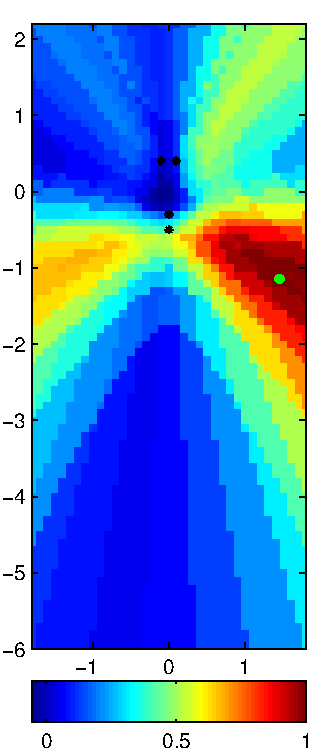
\includegraphics[width=\textwidth]{Pattern_Fo1500_pos01}
\label{fig:Pattern_Fo1500_pos01}
      \end{subfigure}
\begin{subfigure}[t]{0.3\textwidth}
        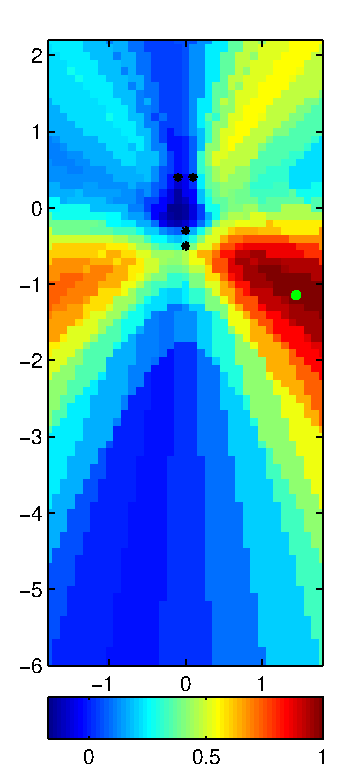
\includegraphics[width=\textwidth]{SRP_Fo1500_frame003_pos01}
\label{fig:SRP_Fo1500_pos01}
      \end{subfigure}
\begin{subfigure}[t]{0.3\textwidth}
        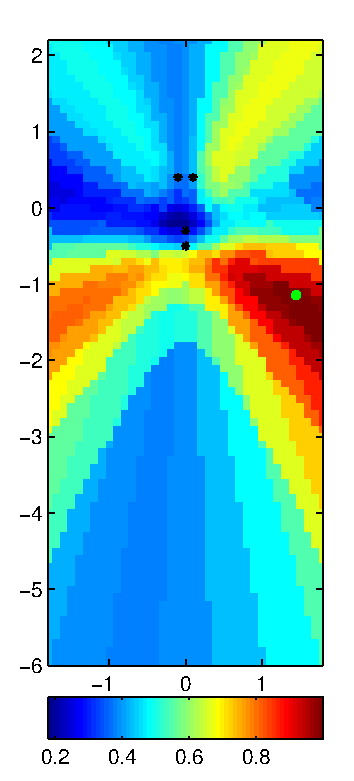
\includegraphics[width=\textwidth]{SRP_Fo1500_mean_pos01}
\label{fig:SRP_Fo1500_mean_pos01}
      \end{subfigure}
      \vspace{\verticalSpacingSRPMaps}
      \caption{\centering For position 1}
      \label{fig:SRPvsModel_Fo1500_position1}
      \vspace{0.25cm}
    \end{minipage}
  \end{subfigure}
  ~\begin{subfigure}[t]{0.47\textwidth}
    \begin{minipage}[t]{\textwidth}
      \begin{subfigure}[t]{0.3\textwidth}
        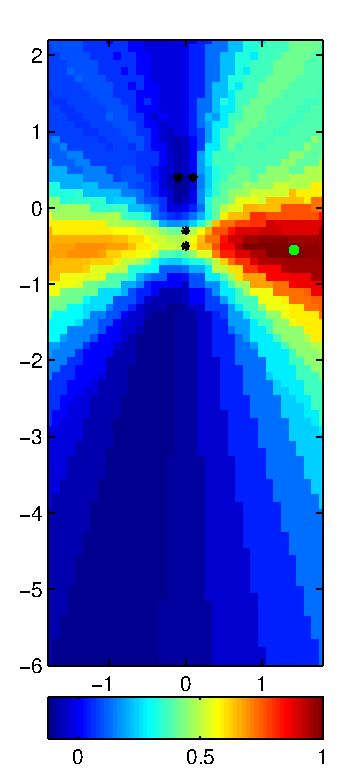
\includegraphics[width=\textwidth]{Pattern_Fo1500_pos02}
\label{fig:Pattern_Fo1500_pos02}
      \end{subfigure}
\begin{subfigure}[t]{0.3\textwidth}
        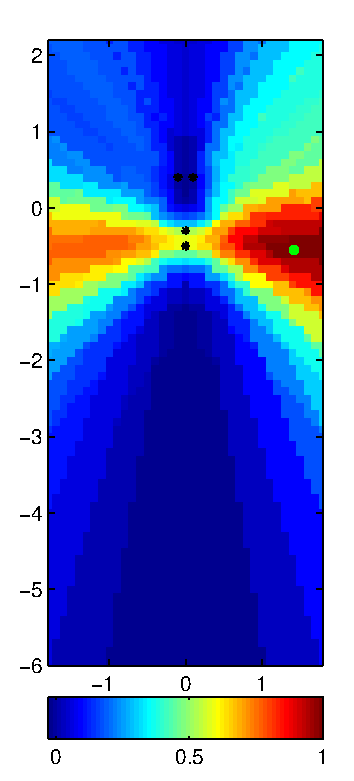
\includegraphics[width=\textwidth]{SRP_Fo1500_frame161_pos02}
\label{fig:SRP_pos02}
      \end{subfigure}
\begin{subfigure}[t]{0.3\textwidth}
        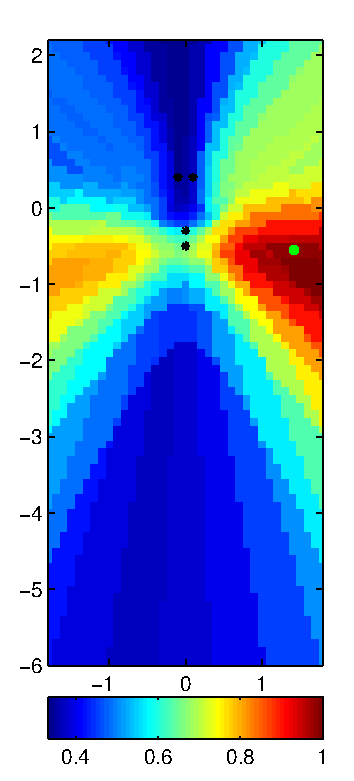
\includegraphics[width=\textwidth]{SRP_Fo1500_mean_pos02}
\label{fig:SRP_Fo1500_mean_pos02}
      \end{subfigure}
      \vspace{\verticalSpacingSRPMaps}
      \caption{\centering For position 2}
      \vspace{0.25cm}
    \end{minipage}
  \end{subfigure}

  \begin{subfigure}[t]{0.47\textwidth}
    \begin{minipage}[t]{\textwidth}
      \begin{subfigure}[t]{0.3\textwidth}
        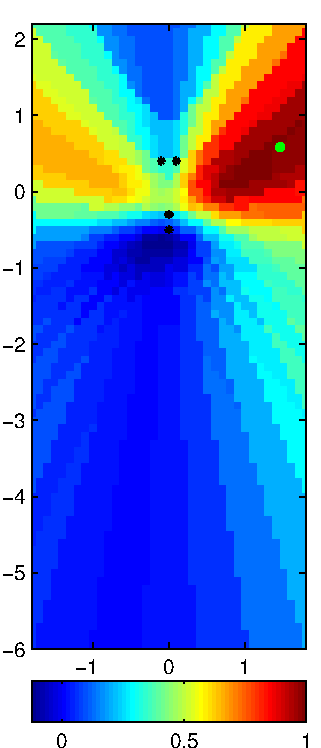
\includegraphics[width=\textwidth]{Pattern_Fo1500_pos04}
\label{fig:Pattern_Fo1500_pos04}
      \end{subfigure}
\begin{subfigure}[t]{0.3\textwidth}
        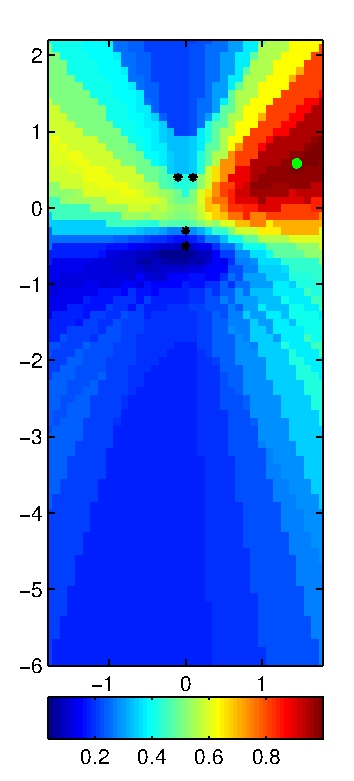
\includegraphics[width=\textwidth]{SRP_Fo1500_frame464_pos04}
\label{fig:SRP_pos04}
      \end{subfigure}
\begin{subfigure}[t]{0.3\textwidth}
        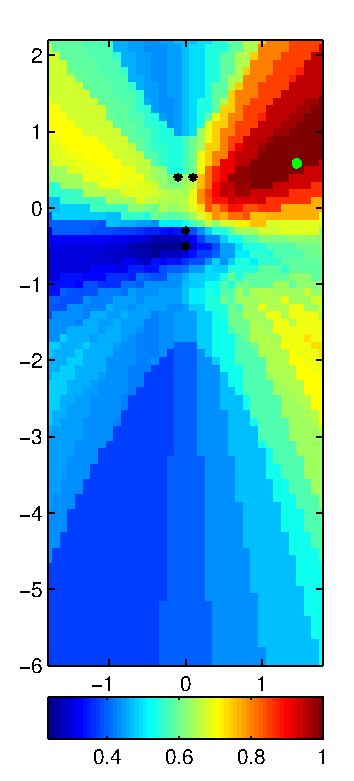
\includegraphics[width=\textwidth]{SRP_Fo1500_mean_pos04}
\label{fig:SRP_Fo1500_mean_pos04}
      \end{subfigure}
      \vspace{\verticalSpacingSRPMaps}
      \caption{\centering For position 4}
      \vspace{0.25cm}
    \end{minipage}
  \end{subfigure}
  ~\begin{subfigure}[t]{0.47\textwidth}
    \begin{minipage}[t]{\textwidth}
      \begin{subfigure}[t]{0.3\textwidth}
        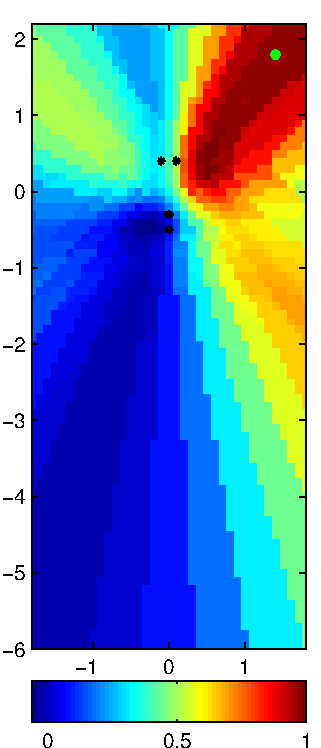
\includegraphics[width=\textwidth]{Pattern_Fo1500_pos06}
\label{fig:Pattern_Fo1500_pos06}
      \end{subfigure}
\begin{subfigure}[t]{0.3\textwidth}
        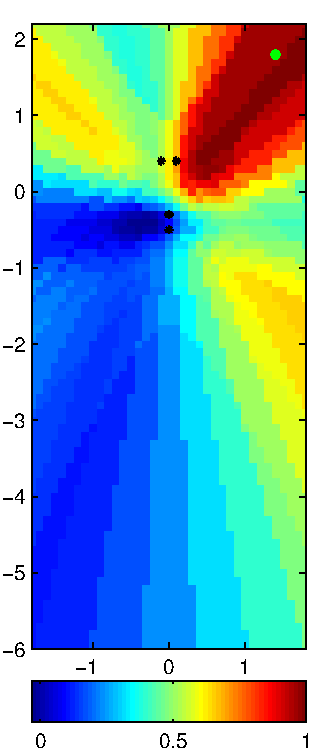
\includegraphics[width=\textwidth]{SRP_Fo1500_frame809_pos06}
\label{fig:SRP_pos06}
      \end{subfigure}
\begin{subfigure}[t]{0.3\textwidth}
        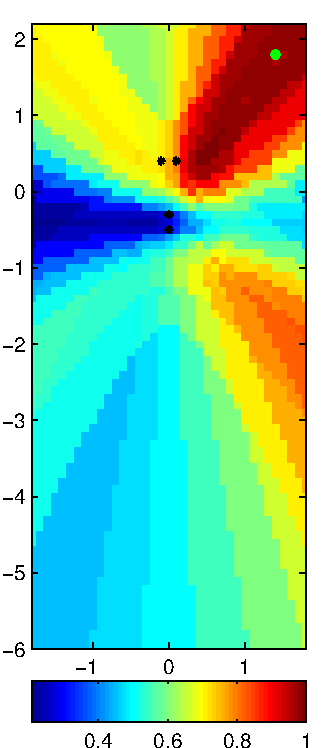
\includegraphics[width=\textwidth]{SRP_Fo1500_mean_pos06}
\label{fig:SRP_Fo1500_mean_pos06}
      \end{subfigure}
      \vspace{\verticalSpacingSRPMaps}
      \caption{\centering For position 6}
      \vspace{0.25cm}
    \end{minipage}
  \end{subfigure}

  \begin{subfigure}[t]{0.47\textwidth}
    \begin{minipage}[t]{\textwidth}
      \begin{subfigure}[t]{0.3\textwidth}
        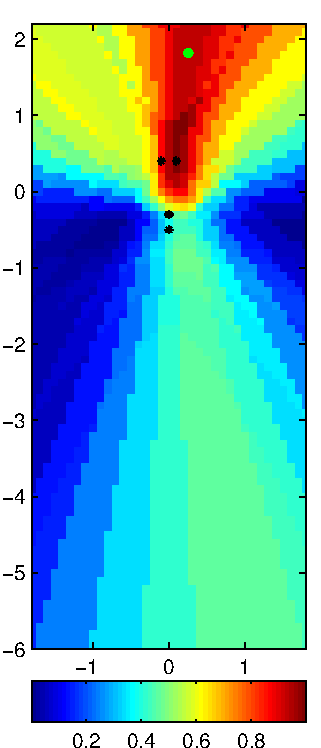
\includegraphics[width=\textwidth]{Pattern_Fo1500_pos08}
\label{fig:Pattern_Fo1500_pos08}
      \end{subfigure}
\begin{subfigure}[t]{0.3\textwidth}
        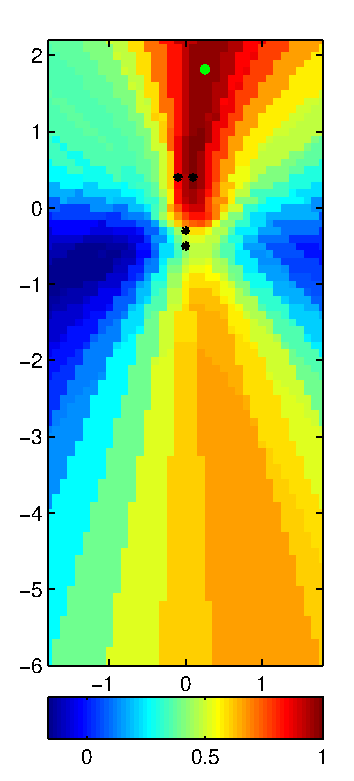
\includegraphics[width=\textwidth]{SRP_Fo1500_frame1127_pos08}
\label{fig:SRP_pos08}
      \end{subfigure}
\begin{subfigure}[t]{0.3\textwidth}
        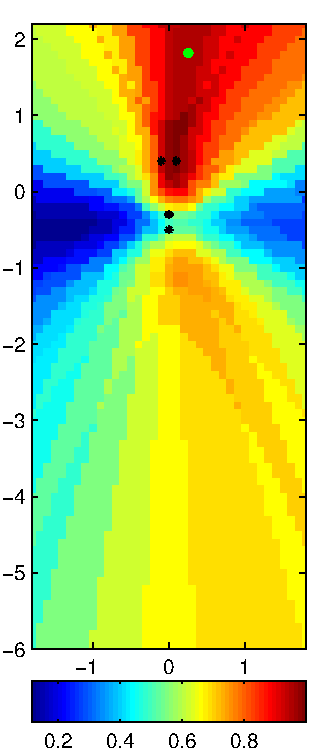
\includegraphics[width=\textwidth]{SRP_Fo1500_mean_pos08}
\label{fig:SRP_Fo1500_mean_pos08}
      \end{subfigure}
      \vspace{\verticalSpacingSRPMaps}
      \caption{\centering For position 8}
      \vspace{0.25cm}
    \end{minipage}
  \end{subfigure}
  ~\begin{subfigure}[t]{0.47\textwidth}
    \begin{minipage}[t]{\textwidth}
      \begin{subfigure}[t]{0.3\textwidth}
        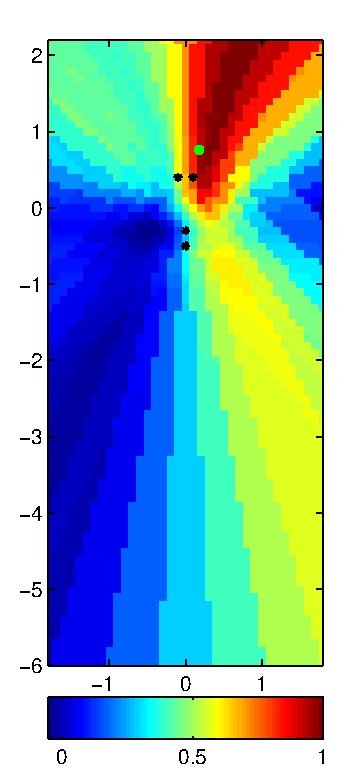
\includegraphics[width=\textwidth]{Pattern_Fo1500_pos16}
\label{fig:Pattern_Fo1500_pos16}
      \end{subfigure}
\begin{subfigure}[t]{0.3\textwidth}
        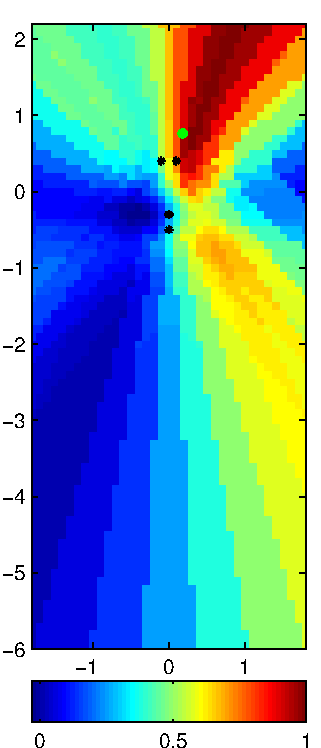
\includegraphics[width=\textwidth]{SRP_Fo1500_frame2518_pos16}
\label{fig:SRP_pos16}
      \end{subfigure}
\begin{subfigure}[t]{0.3\textwidth}
        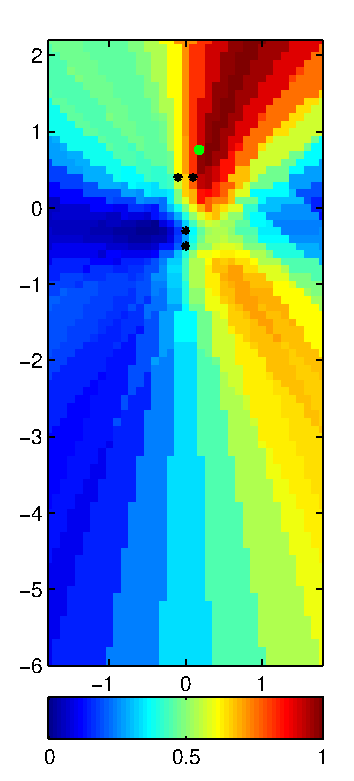
\includegraphics[width=\textwidth]{SRP_Fo1500_mean_pos16}
\label{fig:SRP_Fo1500_mean_pos16}
      \end{subfigure}
      \vspace{\verticalSpacingSRPMaps}
      \caption{\centering For position 16}
      \vspace{0.25cm}
    \end{minipage}
  \end{subfigure}
  \caption{Comparison between the SRP-PHAT map predicted by the model
    (left graphics),
    the real SRP-PHAT map (middle graphics), and the average (real)
    SRP-PHAT map (right graphics), for
    several speaker positions ($f_0=1.5~KHz$). See
    figure~~\ref{fig:simureal_positions}.\subref{fig:real_positions_short}
    for geometrical references.}
  \label{fig:SRPvsPatternSelected}
\end{figure}
 
\begin{wrapfigure}{r}{0.5\textwidth} 
\vspace{-20pt}
  \begin{center}
    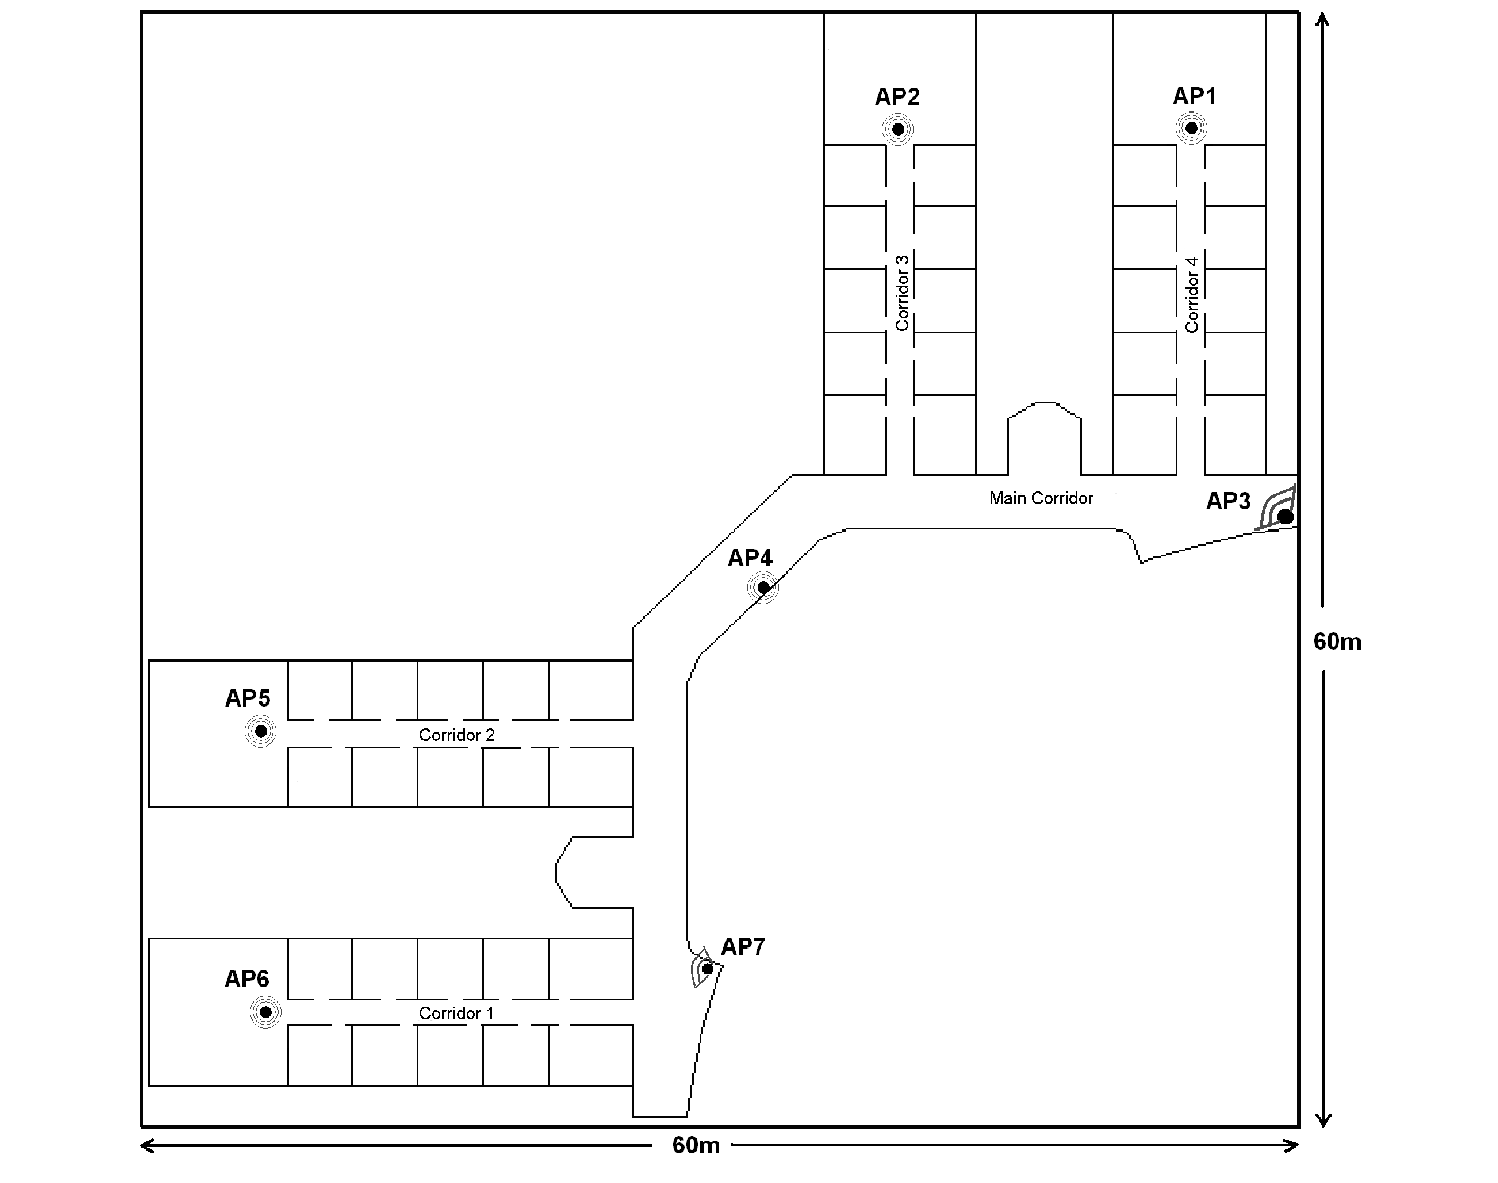
\includegraphics[width=0.4\textwidth]{Figure1}
    \caption{Ejemplo de figura con wrapfigure.}
    \label{fig:wrapfigure1}
  \end{center}
  \vspace{-20pt}
  \vspace{1pt}
\end{wrapfigure} 

Otra posibilidad es utilizar el entorno \texttt{wrapfig} para hacer que
el texto bordee a las figuras, como en la
figura~\ref{fig:wrapfigure1}. Añado ahora unas líneas de loren ipsum
para que lo veáis bien. \lipsum[1-1]





Incluso podemos poner una tabla ``apaisada'', como en la
\ref{tablas2006}, donde se muestra un resumen de los resultados
obtenidos en una serie de experimentos de localización de locutores.

\clearpage
\begin{sidewaystable}[hbtp]
  \begin{center}

    \begin{tabular}{||l|c|c|c|c|c||}
      \hline \hline
      & UKA & ITC & AIT & UPC & IBM\\
      \hline
      \hline
      Pcor & $57.0\pm1.4\%$ & $84.0\pm3.3\%$ & $47.0\pm3.1\%$ & $20.0\pm2.5\%$ & $67.0\pm2.9\%$ \\
      \hline
      Bias fine (x:y:z) [mm] & $20:-42:-75$ & $45:27:-41$ & $-27:-77:-40$ & $-59:112:52$ & $91:-69:-38$ \\
      \hline
      Bias fine+gross (x,y,z) [mm] & $735:-93:-258$ & $67:439:-134$ & $17:-402:-118$ & $-141:255:39$ & $474:-141:-14$ \\
      \hline
      AEE fine [mm] = MOTP & $210$ & $130$ & $266$ & $344$ & $228$ \\
      \hline
      Fine+gross [mm] & $1201$ & $632$ & $1006$ & $1188$ & $884$ \\
      \hline
      Loc. frames & $5035$ & $22$ & $995$ & $977$ & $1023$ \\
      \hline
      Ref. duration (s) & $6287.0$ & $596.0$ & $1143.0$ & $1180.0$ & $1194.0$ \\
      \hline \hline
    \end{tabular}
    \caption{Resultados TEST CLEAR 2006.}
    \label{tablas2006}
  \end{center}
\end{sidewaystable}



\section{Conclusiones}
\label{sec:conclusiones-resultados}

Blah, blah, blah.


 


\chapter{Conclusiones y líneas futuras}
\label{cha:concl-y-line}

En este apartado se resumen las conclusiones obtenidas y se proponen
futuras líneas de investigación que se deriven del trabajo.

La estructura del capítulo es...


\section{Conclusiones}
\label{sec:conclusiones}

Para añadir una referencia a un autor, se puede utilizar el paquete
\texttt{cite}. En el trabajo \cite{armani03}, se muestra un trabajo...

Y podemos usar de nuevo algún acrónimo, como por ejemplo \ac{TDPSOLA}, o
uno ya referenciado como \ac{ANN}.


\section{Líneas futuras}
\label{sec:lineas-futuras}

Pues eso.





 




\chapter{Presupuesto}
\label{cha:presupuesto}

Blah, blah, blah.

 





\bibliographystyle{IEEEtran}

\newcommand{\mybibfileOne}{biblio/biblio.bib}


\newcommand{\mybibfiles}{\myreferencespath\mybibfileOne}


\inputencoding{latin1}
\bibliography{\mybibfiles}
\inputencoding{utf8}




 






\begin{appendices}
  


\chapter{Manual de usuario}
\label{cha:manual-de-usuario}

\section{Introducción}
\label{sec:intro-manual-de-usuario}

Blah, blah, blah\ldots


\section{Manual}
\label{sec:sec-manual-de-usuario}

Pues eso.


\section{Ejemplos de inclusión de fragmentos de código fuente}
\label{sec:codigo-fuente}

Para la inclusión de código fuente se utiliza el paquete
\texttt{listings}, para el que se han definido algunos estilos de
ejemplo que pueden verse en el fichero \texttt{Config/preamble.tex} y
que se usan a continuación.

Así se inserta código fuente, usando el estilo \texttt{CppExample} que
hemos definido en el preamble, escribiendo el código directamente :

\begin{lstlisting}[style=CppExample]
#include <stdio.h>

// Esto es una funcion de prueba
void funcionPrueba(int argumento)
{	
	int prueba = 1;

  printf("Esto es una prueba [

}
\end{lstlisting}

O bien insertando directamente código de un fichero externo, como en el
ejemplo \ref{cod:sample1}, usando
\texttt{\textbackslash{}lstinputlisting} y cambiando el estilo a
\texttt{Cbluebox} (además de usar el entorno \texttt{codefloat} para
evitar pagebreaks, etc.).

\begin{codefloat}
\inputencoding{latin1}
\lstinputlisting[style=Cbluebox]{appendix/function.c}
\inputencoding{utf8}
\caption{Ejemplo de código fuente con un \texttt{lstinputlisting} dentro
de un \texttt{codefloat}}
\label{cod:sample1}
\end{codefloat}


O por ejemplo en matlab, definiendo settings en lugar de usar estilos
definidos:

\lstset{language=matlab}
\lstset{tabsize=2}
\lstset{commentstyle=\textit}
\lstset{stringstyle=\ttfamily, basicstyle=\small}
\begin{lstlisting}[frame=trbl]{}
a = 9;
b = 10;

c = a+b;

fprintf(1, 'La suma de \end{lstlisting}

O incluso como en el listado \ref{cod:sample2}, usando un layout más refinado (con
los settings de \url{http://www.rafalinux.com/?p=599} en un \texttt{lststyle}
\texttt{Cnice}).


\begin{codefloat}
\lstinputlisting[style=Cnice]{appendix/hello.c}
\caption{Ejemplo de código fuente con estilo \texttt{Cnice}, de nuevo
  con un \texttt{lstinputlisting} dentro de un \texttt{codefloat}}
\label{cod:sample2}
\end{codefloat}

Y podemos reutilizar estilos cambiando algún parámetro, como podemos ver
en el listado \ref{cod:sample3}, en el que hemos vuelto a usar el estilo
\texttt{Cnice} eliminando la numeración.


\begin{codefloat}
\lstinputlisting[style=Cnice,numbers=none]{appendix/hello.c}
\caption{Ejemplo de código fuente con estilo \texttt{Cnice}, modificado
para que no aparezca la numeración.}
\label{cod:sample3}
\end{codefloat}


\noindent
Ahora compila usando \texttt{gcc}:


\begin{lstlisting}[style=console, numbers=none]
$ gcc  -o hello hello.c
\end{lstlisting}

Y también podemos poner ejemplos de código \textit{coloreado}, como se
muestra en el \ref{cod:sample5}.

\begin{codefloat}
\lstinputlisting[style=Ccolor]{appendix/hello.c}
\caption{Ejemplo con colores usando el estilo \texttt{Ccolor}}
\label{cod:sample5}
\end{codefloat}

Finalmente aquí tenéis un ejemplo de código shell, usando el estilo
\texttt{BashInputStyle}:

\begin{lstlisting}[style=BashInputStyle, numbers=none]
#!/bin/sh

HOSTS_ALL="gc000 gc001 gc002 gc003 gc004 gc005 gc006 gc007"

for h in $HOSTS_ALL
do
	echo "Running [$*] in $h..."
  echo -n "   "
  ssh root@$h $*
done
\end{lstlisting}


\section{Ejemplos de inclusión de algoritmos}
\label{sec:algoritmos}

Desde la versión de abril de 2014, empezamos a usar el paquete
\texttt{algorithm2e} para incluir algoritmos, y hay ajustes específicos
y dependientes de este paquete tanto en \texttt{Config/preamble.tex}
como en \texttt{cover/extralistings.tex} (editadlos según vuestras
necesidades). 

Hay otras opciones disponibles (por ejemplo las descritas en
\url{http://en.wikibooks.org/wiki/LaTeX/Algorithm}), y podemos
abordarlas, pero por el momento nos quedamos con \texttt{algorithm2e}.

Incluimos dos ejemplos directamente del manual: uno sencillo en el
algoritmo~\ref{alg:howto}, y otro un poco más complicado en el
algoritmo~\ref{alg:restriction}.

\begin{algorithm}[H]
 \caption{How to write algorithms}
 \label{alg:howto}
 \KwData{this text}
 \KwResult{how to write algorithm with \LaTeX2e }
 initialization\;
 \While{not at end of this document}{
  read current\;
  \eIf{understand}{
   go to next section\;
   current section becomes this one\;
   }{
   go back to the beginning of current section\;
  }
 }
\end{algorithm}


\begin{algorithm}
  \caption{IntervalRestriction\label{IR}}
  \label{alg:restriction}
  \DontPrintSemicolon
\KwData{$G=(X,U)$ such that $G^{tc}$ is an order.}
  \KwResult{$G'=(X,V)$ with $V\subseteq U$ such that $G'^{tc}$ is an
    interval order.}
  \Begin{
    $V \longleftarrow U$\;
    $S \longleftarrow \emptyset$\;
    \For{$x\in X$}{
      $NbSuccInS(x) \longleftarrow 0$\;
      $NbPredInMin(x) \longleftarrow 0$\;
      $NbPredNotInMin(x) \longleftarrow |ImPred(x)|$\;
    }
    \For{$x \in X$}{
      \If{$NbPredInMin(x) = 0$ {\bf and} $NbPredNotInMin(x) = 0$}{
        $AppendToMin(x)$}
    }
    \nl\While{$S \neq \emptyset$}{\label{InRes1}
      \nlset{REM} remove $x$ from the list of $T$ of maximal index\;\label{InResR}
      \lnl{InRes2}\While{$|S \cap ImSucc(x)| \neq |S|$}{
        \For{$ y \in S-ImSucc(x)$}{
          \{ remove from $V$ all the arcs $zy$ : \}\;
          \For{$z \in ImPred(y) \cap Min$}{
            remove the arc $zy$ from $V$\;
            $NbSuccInS(z) \longleftarrow NbSuccInS(z) - 1$\;
            move $z$ in $T$ to the list preceding its present list\;
            \{i.e. If $z \in T[k]$, move $z$ from $T[k]$ to
            $T[k-1]$\}\;
          }
          $NbPredInMin(y) \longleftarrow 0$\;
          $NbPredNotInMin(y) \longleftarrow 0$\;
          $S \longleftarrow S - \{y\}$\;
          $AppendToMin(y)$\;
        }
      }
      $RemoveFromMin(x)$\;
    }
  }
\end{algorithm}




   

\chapter{Herramientas y recursos}
\label{cha:herr-y-recurs}

Las herramientas necesarias para la elaboración del proyecto han sido:

\begin{itemize}
\item PC compatible 
\item Sistema operativo GNU/Linux \cite{gnulinux}
\item Entorno de desarrollo Emacs \cite{emacs}
\item Entorno de desarrollo KDevelop \cite{kdevelop}
\item Procesador de textos \LaTeX \cite{lamport94}
\item Lenguaje de procesamiento matemático Octave  \cite{octave}
\item Control de versiones CVS \cite{cvs}
\item Compilador C/C++ gcc \cite{gcc}
\item Gestor de compilaciones make \cite{make}
\end{itemize}




   

\chapter{Versiones}
\label{cha:versiones}

En este apartado incluyo el historial de cambios más relevantes de la
plantilla a lo largo del tiempo.

No empecé este apéndice hasta principios de 2015, con lo que se ha
perdido parte de la información de los cambios importantes que ha ido
sufriendo esta plantilla.


\begin{itemize}

  
\item Julio 2021
  \begin{itemize}
    
  \item El salto gigante desde el 2015 no es porque no haya ido
    haciendo cambios, pero no he tenido el tiempo necesario para
    documentarlos.
    
  \item Ahora la plantilla está accesible de dos formas:
    \begin{itemize}
    
    \item En github, por si a los que lo queráis usar os es más fácil
      clonar o hacer un fork. Está disponible en
      \url{https://github.com/JaviMaciasG/PhD-TFM-TFG-LatexTemplate} y
      podéis clonarlo desde
      \url{https://github.com/JaviMaciasG/PhD-TFM-TFG-LatexTemplate.git}. Ojo
      que tiene morralla variada que puede que no os interese.
    \item En mi dropbox, en formatos zip y tgz, accesible en
      \url{https://www.dropbox.com/sh/mm6fwh3ruuuyjz2/AABDUmo7Xj1S968FeJgbmFPva?dl=0}
      y sin la morralla que os decía.
      
    \end{itemize}
    
  \item Reestructuración completa de la estructura de directorios
  \item Soporte para el manejo adecuado de los ``géneros'', para lo
    que hay que definirlos en el fichero de configuración. Creo que es
    completo, pero si veis algún error, dadme un toque.
  \item Soporte completo (por fin) de utf-8, salvo en los ficheros
    .bib que no lo he conseguido.    
  \end{itemize}
  
\item Mayo 2015:
  \begin{itemize}
  \item Hay disponible un \texttt{make bare} para que deje los capítulos
    mondos y lirondos y se pueda escribir desde casi cero sin tener que
    andar borrando manualmente.
  \end{itemize}


\item Abril 2015:
  \begin{itemize}
  \item Ahora manejamos masculino/femenino en algunos sitios (el/la,
    autor/autora, alumno/alumna, del/de la, ...). Hay que definir
    variable con el género del autor (todavía queda pendiente lo de los
    tutores y tal). NOT FINISHED!!
  \end{itemize}


\item Enero 2015:
  \begin{itemize}
  \item Solucionado el problema (gordo) de compilación del
    \texttt{anteproyecto.tex} y el \texttt{book.tex}, debido al uso de
    paths distintos en la compilación de la bibliografía. El sistema se ha
    complicado un poco (ver
    \texttt{biblio\textbackslash{}bibliography.tex}).
  \item Añadido un (rudimentario) sistema para generar pdf con las
    diferencias entre el documento en su estado actual y lo último
    disponible en el repositorio (usando \texttt{latexdiff}).
  \end{itemize}
\item Diciembre 2015:
  \begin{itemize}
  \item Separada la compilación del anteproyecto de la del documento
    principal. Para el primero se ha creado el directorio
    \texttt{anteproyecto} donde está todo lo necesario.
  \end{itemize}
\end{itemize}




 \end{appendices}


\backmatter                                       





\ifthenelse{\equal{\mybookworktype}{TFG}}
{
  

\chapter*{ }
\thispagestyle{empty}

\cleartoleftpage
\thispagestyle{empty}

\BgThispage



\begin{tikzpicture}[remember picture,overlay]
    \node[yshift=-5cm] at (current page.north west)
      {
        \begin{tikzpicture}[remember picture, overlay]
          \draw[fill=headingPortadaTFG,headingPortadaTFG] (0,0) rectangle (\paperwidth,5cm);

          \node [yshift=3cm, xshift=0.5\paperwidth, font=\Huge, text centered, midway] {\color{textoHeadingPortadaTFG}\myUniversity};
          \node [yshift=2cm, xshift=0.5\paperwidth, font=\Huge, text centered, midway] {\color{textoHeadingPortadaTFG}\mySchool};

        \end{tikzpicture}
      };
   \end{tikzpicture}


\large
\vspace{20cm}
\begin{center}
  
  \centerline{
\includegraphics[height=2.5cm]{uah/01_logo-vA_pant293.pdf}}

\end{center}






 }
{
\ifthenelse{\equal{\mybookworktype}{TFM}}
{
  

\chapter*{ }
\thispagestyle{empty}

\cleartoleftpage
\thispagestyle{empty}

\BgThispage



\begin{tikzpicture}[remember picture,overlay]
    \node[yshift=-5cm] at (current page.north west)
      {
        \begin{tikzpicture}[remember picture, overlay]
          \draw[fill=headingPortadaTFG,headingPortadaTFG] (0,0) rectangle (\paperwidth,5cm);

          \node [yshift=3cm, xshift=0.5\paperwidth, font=\Huge, text centered, midway] {\color{textoHeadingPortadaTFG}\myUniversity};
          \node [yshift=2cm, xshift=0.5\paperwidth, font=\Huge, text centered, midway] {\color{textoHeadingPortadaTFG}\mySchool};

        \end{tikzpicture}
      };
   \end{tikzpicture}


\large
\vspace{20cm}
\begin{center}
  
  \centerline{
\includegraphics[height=2.5cm]{uah/01_logo-vA_pant293.pdf}}

\end{center}






 }
{
}
}




 

\end{document}
